%%
%% Template of the department Very Large Business Applications,
%%    CvO University Oldenburg for scientific papers
%%
%% Created by Dipl.-Inform. Daniel Süpke
%%    For questions, comments, suggestions etc. send an email to:
%%    suepke@wi-ol.de or suepke@gmx.de
%%
%% Version: April 16, 2010
%%
%% Note: Has only been tested with pdflatex, not latex (dvi). Still, there is
%% theoretical support also for latex.
%%
\documentclass[enabledeprecatedfontcommands,12pt]{scrartcl}

%% packages
\usepackage[utf8]{inputenc}       % Standard for Linux
%\usepackage[latin1]{inputenc}    % Standard for Windows
\usepackage{ngerman}              % For German language
\usepackage{fancyhdr}
\usepackage{geometry}
\usepackage{ifpdf}
\usepackage{setspace}             % For line spread
\usepackage[printonlyused, withpage, smaller]{acronym}
\usepackage[authoryear, round, sort]{natbib}
\usepackage{csquotes}
\renewcommand{\mkbegdispquote}[2]{\itshape}
\usepackage{enumitem}
\usepackage[table]{xcolor}
\usepackage{color}

% For pdflatex
\ifpdf
  % One of these two:
  \usepackage[pdftex]{graphicx}
  %\usepackage[pdftex]{epsfig}

  \usepackage[pdftex]{hyperref}
% For latex (dvi)
\else
  % One of these two:
  \usepackage[dvips]{graphicx}
  %\usepackage[dvips]{epsfig}

  % make the command \href from hyperref available as a 'print only'
  \newcommand{\href}[2]{#2}
\fi

%% Picture options
\graphicspath{{pictures/}}         % Default path to pictures used
\DeclareGraphicsExtensions{.png}   % More extensions can be added

% Hyper ref coloring
\hypersetup{colorlinks, citecolor=black, linkcolor= black, urlcolor=black}

%% Pagestyle options
\pagestyle{fancy}
%\lhead{}
%\chead{}
%\rhead{}
%\lfoot{Daniel Süpke}
%\cfoot{}
%\rfoot{}
\renewcommand{\headrulewidth}{0.4pt}

\geometry{a4paper,left=3cm,right=3cm}
%\geometry{a4paper,left=3cm,right=2.5cm}   % Please use these settings for a PhD-thesis

%% Document start
\begin{document}

\pagenumbering{Roman}

% Insert titlepage
%% Title page
\begin{titlepage}
  \begin{centering}
  \begin{figure}[h!]
    \centering
    
\includegraphics[width=310pt]{CvO-Oldenburg-Logo}    % Ggf. Copyright beachten - ansonsten nur für Gebrauch an der CvO
  \end{figure}

  \vspace*{-0.8cm}

  \begin{figure}[h!]
    \centering
    
\includegraphics[width=250pt]{VLBA_waagerecht}    % Ggf. Copyright beachten - ansonsten nur für Gebrauch an der CvO/VLBA
  \end{figure}

  \vspace*{0.4cm}
  
  \textsf{\Huge \textbf{Cloud Computing, Internet of Things, Industrie 4.0, Predictive Maintenance, SCADA, SAP HANA\\}}

  \vspace*{0.5cm}
  \noindent Masterarbeit\\

  \end{centering}
  
  \vspace*{1.5cm}
  \begin{tabbing}
  xxxxxxxxxxxxxxxx\= \kill
  
  % Change me
  \small Themensteller:\> Prof. Dr.-Ing. Jorge Marx Gómez\\
  \small Betreuer:\> Prof. Dr.-Ing. Hergen Pargmann\\\\

  \small Vorgelegt von: \>Nils Lutz\\
  \small \>Erlenweg 5\\
  \small \>26129 Oldenburg\\
  \small \>+49 173 25 28 407\\
  \small \>nils.lutz@uni-oldenburg.de\\\\

  \small Abgabetermin:\> 30. April 2017
  \end{tabbing}
\end{titlepage}
%\thispagestyle{empty}
\newpage

% Insert table of contents
% Insert table of contents
\tableofcontents
\newpage

% Insert glossary, table of symbols, list of figures and list of tables
\section*{Akronyme}            % Alternatively a glossary package can be used
\addcontentsline{toc}{section}{Akronyme}
\begin{acronym}[HACCP]
  \acro{api}[API]{Application Programming Interface}
	\acro{baas}[BaaS]{Blockchain-as-a-Service}
  \acro{bft}[BFT]{Byzantine Fault Tolerant}
  \acro{bna}[BNA]{Business Network Archive}
  \acro{brc}[BRC]{British Retail Consortium}
	\acro{btc}[BTC]{Bitcoin}
  \acro{ca}[CA]{Certificate Authority}
  \acro{cli}[CLI]{Command Line Interface}
	\acro{dena}[dena]{Deutsche Energie-Agentur}
	\acro{dlt}[DLT]{Distributed Ledger Technology}
  \acro{dsgvo}[DSGVO]{Datenschutz-Grundverordnung}
  \acro{edi}[EDI]{Electronic Data Interchange}
  \acro{erp}[ERP]{Enterprise Resource Planning}
  \acro{gbt}[GBT]{Global Batch Traceability}
  \acro{gfsi}[GFSI]{Global Food Safety Initiative}
  \acro{gln}[GLN]{Global Location Number}
  \acro{gps}[GPS]{Global Positioning System}
  \acro{haccp}[HACCP]{Hazard Analysis and Critical Control Points}
  \acro{hmsc}[HMSC]{Halal Meat Supply Chain}
  \acro{http}[HTTP]{Hypertext Transfer Protocol}
  \acro{idoc}[IDoc]{Intermediate Document}
  \acro{ifs}[IFS]{International Food Standard}
  \acro{iln}[ILN]{Internationale Lokationsnummer}
	\acro{iot}[IoT]{Internet of Things}
  \acro{ki}[KI]{künstliche Intelligenz}
  \acro{lkv}[LKV]{Los-Kennzeichnungs-Verordnung}
  \acro{lmbg}[LMBG]{Lebensmittel- und Bedarfsgegenständegesetz}
  \acro{lmkv}[LMKV]{Lebensmittelkennzeichnungsverordnung}
	\acro{ml}[ML]{Machine Learning}
  \acro{msp}[MSP]{Member Ship Provider}
  \acro{pbft}[pBFT]{Practical Byzantine Fault Tolerant}
  \acro{pki}[PKI]{Public-Key-Infrastructure}
  \acro{poet}[PoET]{Proof-of-Elapsed-Time}
  \acro{pos}[PoS]{Proof-of-Stake}
  \acro{posp}[PoSp]{Proof-of-Space}
	\acro{pow}[PoW]{Proof-of-Work}
  \acro{reif}[REIF]{Resource-Efficent, Economic and Intelligent Foodchain}
  \acro{rest}[REST]{Representational State Transfer}
  \acro{rfid}[RFID]{Radiofrequenz-Identifikation}
	\acro{sc}[SC]{Smart Contract}
  \acro{sql}[SQL]{Structured Query Language}
  \acro{tls}[TLS]{Transport Layer Security}
  \acro{tms}[TMS]{Transportation Management System}
  \acro{ui}[UI]{User Interface}
  \acro{uri}[URI]{Uniform Resource Identifier}
  \acro{vvvo}[VVVO]{Vieh-Verkehrs-Verordnung}
  \acro{wms}[WMS]{Wharehouse Management System}
  \acro{xml}[XML]{Extensible Markup Language}
\end{acronym}

% \section*{Symbolverzeichnis}   % If needed
% \addcontentsline{toc}{section}{Symbolverzeichnis}
\newpage

\listoffigures
\addcontentsline{toc}{section}{Abbildungsverzeichnis}
\listoftables
\addcontentsline{toc}{section}{Tabellenverzeichnis}
\lstlistoflistings
\addcontentsline{toc}{section}{Quelltextverzeichnis}
\newpage


\pagenumbering{arabic}

%% Line spread
\onehalfspacing

% Insert introduction
\section{Motivation}

Industrie 4.0 ist ein Treiber der Digitalisierung vor allem im Bereich der Energiewirtschaft. \cite[vgl.]{UnternehmensbetreuungmbH2017} Durch den Einsatz von Industrie 4.0 sind Unternehmen in der Lage ihre Prozesse und Anlagen in Echtzeit Kontrollieren und Steuern zu können. Dadurch lassen sich Kosten optimieren und die Produktivität steigern. Industrie 4.0 ist der Oberbegriff für eine viel zahl von Technologien.\\
Eine Technologie die bereits heute neue innovative Ideen im privaten Sektor hervorgebracht hat, erobert den industriellen Sektor - Blockchain. Eine Blockchain ist eine verteilte Datenstruktur kombiniert mit Kryptographischen Methoden zur Sicherstellung der Unveränderbarkeit der Daten. Blockchains zählen zu den \ac{dlt}. So erwägen einige der größten Finanzinstitutionen den Einsatz von \ac{dlt}.\cite{Goldman2018}\cite{JPMorgan2018}\\

“Es ist davon auszugehen, dass wir in ein bis zwei Jahrzehnten wirtschaftlich über Mechanismen miteinander interagieren werden, für die wir bislang weder Konzepte noch Begriffe haben.” \cite[S.~92]{Platzer2014} Auch die Deutsche Bundesregierung ist an der Blockchain Technologie interessiert und erwägt den Einsatz in der Zukunft für die unterschiedlichsten Services. In einer der jüngsten Pressemitteilungen hat der Blockchain Bundesverband mitgeteilt, dass die Regierung eine umfassende Strategie zum Umgang und Einsatz der Technologie erarbeiten will. \cite{BCBundesverband2018}

\begin{figure}[h!]
	\centering
	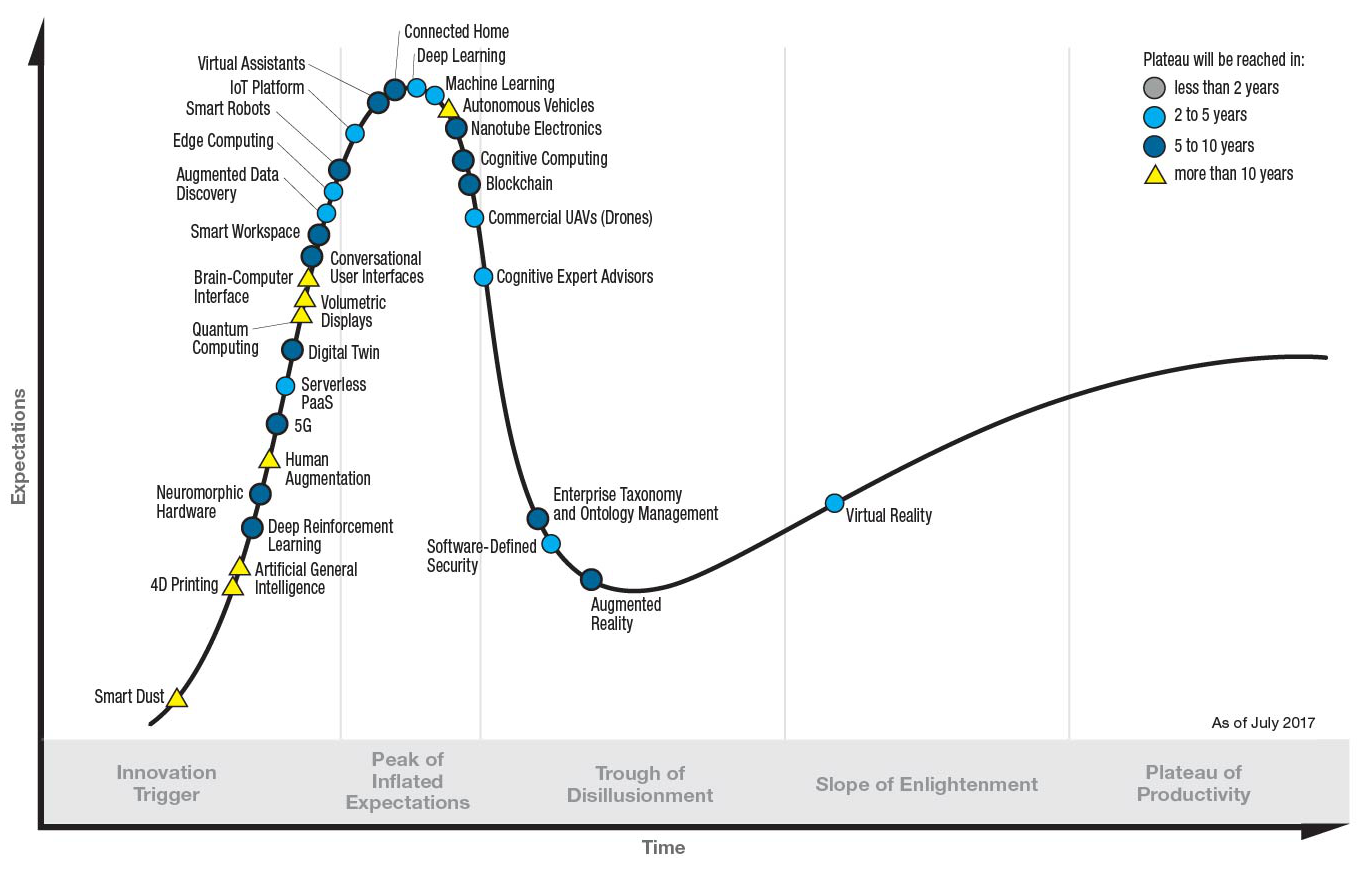
\includegraphics[width=0.65\linewidth]{pictures/Gartner-Hype-Cycle-2017}
	\caption[Gartner Hype Cycle 2017]{Emerging Technologies Hype Cycle 2017\cite{Gartner2017}}
	\label{fig:gartner-hype-cycle-2017}
\end{figure}

Noch ist die Blockchain kein Alltag, bemessen am jährlich erscheinenden Hype Cycle des Marktforschungsinstituts Gartner, Inc. $( Abb.~ \ref{fig:gartner-hype-cycle-2017} )$ hat die Technologie noch fünf bis zehn Jahre Entwicklungszeit vor sich. Erst dann wird sie nach aktueller Einschätzung im produktiven Einsatz sein. Was der Hype Cycle nicht aussagt ist welchen Einfluss die Blockchain auf eine Branche oder die Gesellschaft hat in ihrer jeweiligen Phase.\\

Bereits heute zeigen sich signifikante Unterschiede zwischen den unzähligen Blockchains die in Pilotprojekten realisiert wurden. So gibt es Anwendungen der Blockchain um beispielsweise den Kilometerstand eines Fahrzeugs täglich \glqq in die Blockchain\grqq~ zu schreiben. Die inhärenten Eigenschaften der Blockchain ermöglichen es sehr einfach festzustellen, ob ein Kilometerstand nachträglich durch Fremdeinwirkung manipuliert wurde. Ebenfalls ist keine zentrale Zwischenstelle mehr nötig, um für die Echtheit des hinterlegten Wertes zu garantieren. \cite{carVertical}\\

Bitcoin war die erste Generation von Blockchain. Die Bitcoin Blockchain ist in der Lage Einheiten der Bitcoin Währung zwischen zwei Parteien zu versenden ohne das eine Bank oder eine Clearingstelle diese Transaktion validieren muss. \cite[vgl.]{Nakamoto2009} Ethereum war die zweite Generation einer Blockchain. Im Vergleich zur Bitcoin Blockchain lassen sich mit dem Ethereum Netzwerk auch sog. \ac{sc} erstellen und ausführen.\cite[vgl.]{Buterin2014} Mittlerweile behaupten die ersten Projekte von sich zur dritten Generation von Blockchains zu gehören. Skalierbarkeit und Interoperabilität spielen in dieser Generation eine der entscheidenden Rollen. \cite[vgl.]{Cardano} Auch die Blockchain Anwendungen im Enterprise Bereich lassen in Masse noch auf sich warten. Es fehlen Erfahrungen und konkrete Einsatzgebiete für die Technologie.

\newpage


% Insert body
\section{Verwandte Arbeiten} \label{sec:related-work}
In diesem Kapitel soll ein kurzer Überblick über zwei vorhandene Lösungen im Bereich der Lebensmittelsicherheit und Supply Chain gegeben werden. Im Fokus der Betrachtung liegt die jeweils verwendete Blockchain-Technologie für den spezifischen Use-Case, sowie die tatsächliche Umsetzung und der Stand der Lösung.

\subsection{Thunfisch Traceability}
Der World Wildlife Fund (WWF) in Australien, Fidschi und Neuseeland hat in Zusammenarbeit mit dem US-amerikanischen Technologie-Innovator ConsenSys, dem Technologie-Implementierer TraSeable und dem Thunfischfang- und -verarbeitungs\-unternehmen Sea Quest Fiji Ltd., ein Pilotprojekt in der Thunfischindustrie der Pazifikinseln gestartet, das mit Hilfe der Blockchain-Technologie den Weg des Thunfisches vom \glqq Köder auf den Teller\grqq{} verfolgen wird. Ziel ist es, dazu beizutragen, illegale, nicht gemeldete und unregulierte Fischerei und Menschenrechtsverletzungen in der Thunfischindustrie zu stoppen. Dazu gehören Berichte über Korruption, illegalen Handel und menschliche Sklaverei auf Thunfischfängern.

Das WWF-Pilotprojekt wird eine Kombination aus RFID-Tags (Radio Frequency Identification), QR-Code-Tags (Quick Response) und Lesegeräten verwenden, um Informationen über die Reise eines Thunfisches an verschiedenen Punkten der Lieferkette zu sammeln. Während dieser Technologieeinsatz für das Supply-Chain-Tracking nicht neu ist, ist der innovative Teil, dass die gesammelten Informationen dann mit Hilfe der Blockchain-Technologie aufgezeichnet werden. Die Ortung beginnt, sobald der Thunfisch gefangen wird. Sobald ein Fisch gelandet ist, wird er mit einem wiederverwendbaren RFID-Tag auf dem Schiff befestigt. Geräte, die auf dem Schiff, am Dock und in der Verarbeitungsfabrik angebracht sind, erkennen dann die Tags und laden automatisch Informationen in die Blockchain hoch. 

Nach der Verarbeitung des Fisches wird der wiederverwendbare RFID-Tag gegen einen kostengünstigeren QR-Code ausgetauscht, der an der Produktverpackung angebracht wird. Der eindeutige QR-Code wird mit dem Blockchain-Datensatz verknüpft, der dem jeweiligen Fisch und seinem ursprünglichen RFID-Tag zugeordnet ist. Der QR-Code wird verwendet, um den Rest der Reise des Fisches zum Verbraucher zu verfolgen. Im Moment ist die Verknüpfung von Tags nicht schwierig, da sich das Projekt auf den gesamten Export konzentriert - also den gesamten frischen Fisch abzüglich Kopf, Kiemen und Eingeweiden. Etwas komplizierter wird es, wenn der Fisch in Lenden, Steaks, Würfel und Dosen zerlegt wird, aber das Projektteam ist nun in der Lage, die QR-Code-Tags auf den Verpackungen des verarbeiteten Fisches mit dem Datensatz des Originalfisches auf der Blockkette zu verknüpfen. Auch wenn es möglich sein könnte, RFID-Tags während des gesamten Prozesses zu verwenden, könnten die Kosten dieser Tags kleineren Unternehmen in der Fischwirtschaft die Teilnahme an dem System verbieten, wenn es sich ausweitet. Es besteht auch das Potenzial, in Zukunft mit Nahfeldkommunikationsgeräten (NFC) die Fische bis zum Verbraucher zu verfolgen.

\citep{Visser2017}
\citep{McEntire2019}

\subsection{Halal Food Chain}
Da Lebensmittel zwischen den verschiedenen Akteuren der Lieferkette verstreut sind, wächst die Sorge um die Gewährleistung der Lebensmittelsicherheit durch die Einführung vieler Internet- und Sachtechnologien. Neben der Unsicherheit ist die Möglichkeit, dass Halal-Lebensmittel nicht Halal sind, aufgrund der Fahrstrecke, die viele Handhabungspunkte einschließt, und des anhaltenden Risikos einer Kreuzkontamination mit Nicht-Halal-Materialien größer. Um die Fragen im Zusammenhang mit der strengen Einhaltung des Scharia-Rechts durch Halal-Produkte zu klären, gibt es einige Vorveröffentlichungen in Studien über die Rückverfolgbarkeit von Halal-Fleischprodukten \citep{Mohammed2016}. Als Lösung dafür schlug \citet{Mohamad2016} eine Methode vor, um zu bestimmen, ob das Geflügel nach islamischer Art und Weise unter Verwendung einer Untersuchung der Fleischfarbe geschlachtet wird. \citet{Junaini2008} beschrieben eine mobile Unterstützungsanwendung für Muslime zur Identifizierung des Halal-Status. \citet{Kassim2012} führten ein System ein, um die Informationen von Produkten zu verifizieren und zu erkennen und damit ihren Halal-Status in Echtzeit von einem Echtzeit-Zugriff auf ihre Datenbank zu bestätigen. \citet{SitiSarahMohdBahrudin2011} schlugen eine umfassende und geeignete Tracking \& Tracing-Technologie mit \ac{rfid} vor, um die Integrität des Halal-Produkts aufrechtzuerhalten und die gesamte Lieferkette des Halal-Produktprozesses zu unterstützen. \citet{Tan2012} fanden heraus, dass Technologien wie \ac{tms}, \ac{wms}, \ac{edi} und \ac{gps} bei Halal-Logistikdienstleistern weit verbreitet sind. Außerdem betonte \citet{Tan2012} die Kompatibilität der Tracking \& Tracing-Eigenschaft von \ac{rfid} mit der Halal-Transportrichtlinie. \citet{Mohammed2016} stellen einen Rahmen für die Entwicklung eines \ac{rfid}-fähigen \ac{hmsc}-Netzwerks zur Verbesserung der Rückverfolgbarkeit der Halal-Fleischintegrität in der gesamten Lieferkette vor. Alle zuvor genannten Forschungsarbeiten sind die Idee der Verwendung eines zentralen Systems, das letztlich der einzig denkbare Weg war, um Informationstransparenz entlang der Lieferketten zu erreichen \citep{Tian2017}. Es gibt jedoch nicht genügend Beweise für die Richtigkeit und Vertrauenswürdigkeit der gemeinsamen Informationen im Rückverfolgbarkeitssystem und zwischen den Akteuren der Halal-Fleischlieferkette. Dies führt zu einem undurchsichtigen System, Informationsasymmetrie und vielen anderen Problemen. Das \ac{rfid}-fähige Rückverfolgbarkeitssystem reicht nicht aus, um die Halal-Integrität von Fleisch zu gewährleisten. Das manuelle Abrufen und Speichern von Informationen in der zentralen Datenbank bringt viele Möglichkeiten der Irreführung und Verfälschung mit sich. In ähnlicher Weise ist es problematisch, sicherzustellen, dass die so genannten Halal-Fleischprodukte den islamischen Ernährungsvorschriften entsprechen und frei von irreführenden Herkunftsgeschichten sind.

\newpage

\section{Grundlagen} \label{sec:basics}
\textcolor{red}{Lorem ipsum dolor sit amet, consetetur sadipscing elitr, sed diam nonumy eirmod tempor invidunt ut labore et dolore magna aliquyam erat, sed diam voluptua. Lorem ipsum dolor sit amet, consetetur sadipscing elitr, sed diam nonumy eirmod tempor invidunt ut labore et dolore magna aliquyam erat, sed diam voluptua.}

% Chargenrückverfolgung
\subsection{Chargenrückverfolgung}
\textcolor{red}{Notwendigkeit einer Charge erläutern auf Grund der Gruppierung von vielen Einzelprodukten eben zu einer Charge.}

\subsubsection{Definition Charge}

Eine \textit{Charge} bezeichnet eine Ansammlung eines Produkts, welche unter gleichen Bedingungen produziert wurde. Bei dem Produkt kann es sich beispielsweise um Werkstoffe, Bauteile, Baugruppen oder Endprodukte handeln. Die Begriffe \textit{Los} oder \textit{Partie} werden oft als Synonym für \textit{Charge} verwendet. Einige Branchen sind bei der Produktion auf die Erzeugung definierter \textit{Chargen} zugeschnitten. Diese Chargenproduktion, die auch diskontinuierliche Produktion genannt wird, zeichnet sich durch einen zeitlich unterbrochenen Materialfluss aus. So kann ein Produktionsgefäß mit unterschiedlichen Rohstoffen befüllt und anschließend verarbeitet werden. In der diskontinuierlichen Produktion versteht man daher unter einer \textit{Charge} eine Menge eines Erzeugnisses, welche in einem Produktionsgang gefertigt worden ist und identische Kennzeichen in Bezug auf Materialzusammensetzung, Fertigungsprozess und Produktqualität aufweist. Beispiele hierfür finden sich in der Stahlproduktion, der pharmazeutischen und chemischen sowie in der Lebensmittelindustrie \citep{Guenther2012}.

Inzwischen wird der Begriff der \textit{Charge} aber auch in der kontinuierlichen Produktion verwendet. Die \textit{Charge} wird dabei durch die Berücksichtigung einer oder mehrerer der folgenden Eigenschaften charakterisiert:

\begin{itemize}
  \item Herstellung auf einer Fertigungslinie,
  \item einheitliche Zulieferteile,
  \item homogene Qualität,
  \item gleichbleibende Prozesskette,
  \item identisches Produktionsdatum.
\end{itemize}

Es bleibt festzuhalten, dass die Parameter in der kontinuierlichen Produktion nicht so eindeutig abgrenzbar sind wie in der diskontinuierlichen Produktion. Zudem können in der kontinuierlichen Produktion Schwankungen durch dynamische Prozesse wie Abnutzung von Werkzeugen auftreten, die innerhalb einer definierten \textit{Charge} zu deutlichen Qualitätsunterschieden führen können und so die Praxistauglichkeit der Chargenverfolgung in Frage stellen.

In der für die Lebensmittelindustrie wichtigen \ac{lkv} wird unter einem \textit{Los} \glqq die Gesamtheit von Verkaufseinheiten eines Lebensmittels verstanden, das unter praktisch gleichen Bedingungen erzeugt, hergestellt oder verpackt wurde.\grqq{} \citep{LKV1993}. Dagegen bezeichnen laut Code of Federal Regulation \textit{Los} oder \textit{Charge} \glqq ein oder mehrere Bauteile oder fertige Geräte eines einzigen Typs, Version, Klasse, Größe, Zusammensetzung oder Software Version, welche im wesentlichen unter gleichen Bedingungen hergestellt werden und die innerhalb spezifizierter Grenzen einheitliche Eigenschaften und Qualität haben sollen.\grqq{} \citep{QSR1996}. Somit können auch einzelne Produkte eine \textit{Charge} oder ein \textit{Los} bilden. Im Hinblick auf eine möglichst genaue Eingrenzung bestimmter Produkte beispielsweise bei einer Rückrufaktion sollte eine kleinstmögliche Chargengröße gewählt werden, die im Idealfall nur ein einzelnes Produkt umfasst.

\subsubsection{Einordnung in die Wertschöpfungskette}

Die Chargenverfolgung wird innerhalb des Produktionsprozesses für das Upstream Tracing und in dem Distributionsprozess für das Downstream Tracing eingesetzt. Bei einer gut organisierten Chargenverfolgung im Downstream Prozess behält der Hersteller den Überblick, wo seine Produkte wann gelagert, verkauft und eingesetzt werden und ist so in der Lage, gezielt Rückrufe durchzuführen. Durch die Chargenverfolgung im Upstream Prozess können eventuelle Qualitätsprobleme bis zum Vorlieferanten nachverfolgt werden. Abbildung \ref{fig:wkd-Lebensmittelindustrie} zeigt schematisch die Wertschöpfungskette in der Lebensmittelindustrie. Bei einem optimal eingerichtetem Up- und Downstream Tracing behalten die Hersteller und Konsumenten während der ganzen Wert"-schöpfung einen Überblick wo sich die Waren aktuell im Einsatz befinden.

\begin{figure}[h!]
	\centering
	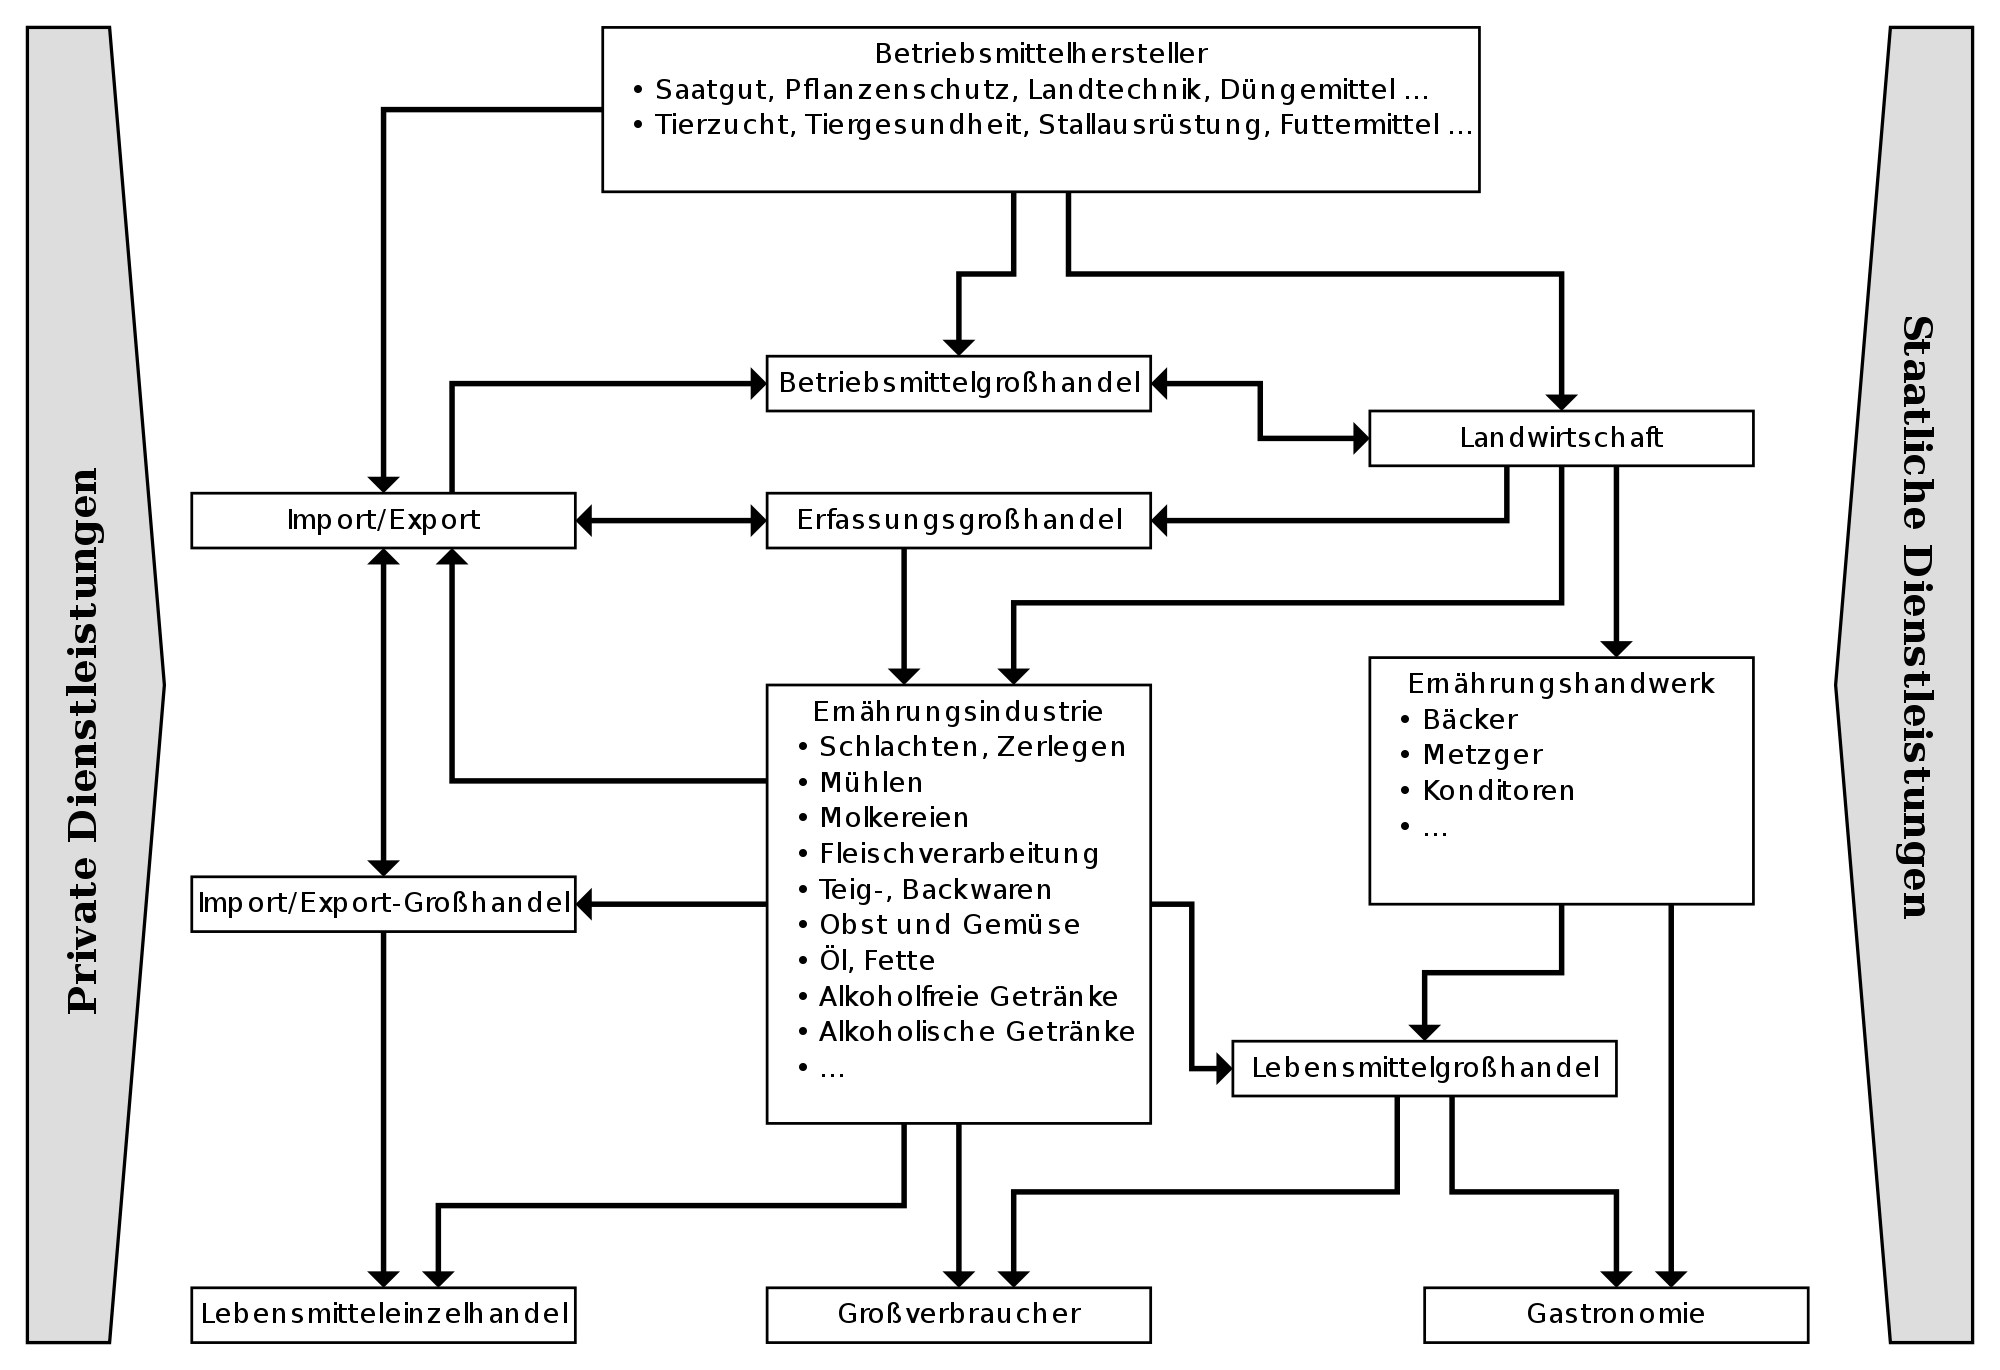
\includegraphics[width=1.0\linewidth]{pictures/system-of-agribusiness}
	\caption[Wertschöpfungskette: Lebensmittelindustrie]{Wertschöpfungskette: Lebensmittelindustrie \textcolor{red}{QUELLE}}
	\label{fig:wkd-Lebensmittelindustrie}
\end{figure}

\paragraph{Downstream Tracing (Abwärts-Rückverfolgbarkeit)}$~~$\\
Als Downstream Tracing wird die Rückverfolgbarkeit ausgehend vom Erzeuger zum Endprodukt bezeichnet. Gegenstand der Rückverfolgung ist typischerweise ein \textit{Los} (\textit{Charge}) oder eine einzelne Einheit eines Produkts. Abhängig vom Grad der Integration innerhalb der Lieferkette lässt sich die Rückverfolgung bis zum Einzelhandel bzw. auch bis zum Endverbraucher durchführen. Zum Einsatz kommt das Downstream Tracing wenn Probleme in Waren zu einem späten Zeitpunkt festgestellt wurden und geprüft werden muss in welchen Endproduktchargen sich hierdurch weitere Probleme ergeben könnten \citep{Trienekens2001, Zailani2010}. \citet{Wegner-Hambloch2004} beschreibt Downstream Tracing als \glqq Ortsbestimmung von bereits hergestellten Produkten zwecks nachträglichen Rückrufs von gesundheitsgefährdenden Produkten\grqq{}.

\paragraph{Upstream Tracing (Aufwärts-Rückverfolgbarkeit)}$~~$\\
Unter Upstream Tracing versteht man die Rückverfolgbarkeit vom Endverbraucher in Richtung des Erzeugers. Tritt ein Problem bei Lebensmittelprodukten auf wird das Upstream Tracing zur Ursachenforschung eingesetzt. So lassen sich Probleme die beispielsweise vom Konsumenten beim Endprodukt oder bei einer Qualitätskontrolle von Teilprodukten festgestellt wurden zurückverfolgen bis zum Urerzeuger \citep{Trienekens2001, Zailani2010}. Nach \citet{Wegner-Hambloch2004} ist Upstream Tracing \glqq die Bestimmung der Produktgeschichte vom Endprodukt [...] bis zu den Futtermitteln.\grqq{}

\subsubsection{Zentrale vs. dezentrale Ansätze}
\textcolor{red}{Unterschied zwischen zentraler Informationssysteme (F-Trace) und dezentraler logischer Systeme (Zugriff auf F-Trace). Letzteres sind nur dem Anschein nach dezentral. Ihre zugrunde liegende Infrastruktur der Informationssysteme ist zentral und wird von einem Intermediär verwaltet und betrieben. Angriffspunkte für Manipulation und Kontrolle eines einzelnen rausarbeiten. \citep{Steins2015, allgemeinefleischerzeitung2011}
Lorem ipsum dolor sit amet, consetetur sadipscing elitr, sed diam nonumy eirmod tempor invidunt ut labore et dolore magna aliquyam erat, sed diam voluptua. At vero eos et accusam et justo duo dolores et ea rebum. Stet clita kasd gubergren, no sea takimata sanctus est Lorem ipsum dolor sit amet. Lorem ipsum dolor sit amet, consetetur sadipscing elitr, sed diam nonumy eirmod tempor invidunt ut labore et dolore magna aliquyam erat, sed diam voluptua. At vero eos et accusam et justo duo dolores et ea rebum. Stet clita kasd gubergren, no sea takimata sanctus est Lorem ipsum dolor sit amet.Lorem ipsum dolor sit amet, consetetur sadipscing elitr, sed diam nonumy eirmod tempor invidunt ut labore et dolore magna aliquyam erat, sed diam voluptua. At vero eos et accusam et justo duo dolores et ea rebum. Stet clita kasd gubergren, no sea takimata sanctus est Lorem ipsum dolor sit amet. Lorem ipsum dolor sit amet, consetetur sadipscing elitr, sed diam nonumy eirmod tempor invidunt ut labore et dolore magna aliquyam erat, sed diam voluptua.}

\subsubsection{Dokumentationspflichten}
Für landwirtschaftliche Waren und daraus hergestellte Nahrungsmittel existieren eine Vielzahl von gesetzlichen Regelungen aus denen Bedingungen und Anforderungen zum Thema Rückverfolgbarkeit abgeleitet werden können. Die VO (EG) Nr. 178/02 \citep{EPER2002} wird in diesem Kontext als Basisverordnung gesehen. Darüber hinaus sind die horizontale Lebensmittelhygieneverordnung sowie die vertikalen Hygieneverordnungen für Fleisch und Fleischerzeugnise, Milch- und Milcherzeugnisse, Fisch und Fischerzeugnisse mit der Vorgabe zur Umsetzung betrieblicher Eigenkontrollen oder Einrichtung eines \acs{haccp}-Systems\footnote{Englisch für \textit{\acf{haccp}}. Beschreibt ein Qualitätskontrollsystem für den sicheren Umgang mit Lebensmitteln durch strukturierte und präventive Maßnahmen zur Verhinderung von Erkrankungen und Verletzungen des Konsumenten.\citep{EPER2004}} elementare Bestandteile eines wirkungsvollen, innerbetrieblichen Rückverfolgungssystems in Lebensmittelbetrieben. Eine verbindliche fünfjährige Speicherung von Daten der Transaktionen bezüglich der Lieferanten und Abnehmer ist ebenfalls festgelegt.\\

\noindent
Weitere Regelungen zur Rückverfolgbarkeit für die EU:
\begin{itemize}
  \item Rindfleischetikettierungs-VO (EWG) Nr. 1760/2000
  \item EU-Öko-VO (EWG) 2092/91
  \item EU-Verordnung über amtliche Futter- und Lebensmittelkontrollen (Vorschlag vom 5. Februar 2003)
  \item Vermarktungsnormen für Eier 1907/90/EWG
\end{itemize}
Nationale Regelungen für Deutschland:
\begin{itemize}
  \item \acf{lmkv}
  \item \acf{lkv}
  \item verschiedene Fleisch- und Geflügelfleisch-Hygienevorschriften
  \item Weingesetz und Weinwirtschaftsgesetz
  \item Handelsklassenrecht
  \item \acf{lmbg}
\end{itemize}
Über die gesetzlichen Regelungen hinaus gelten verbindliche Standards der Handelsseite, die übergreifend von der \ac{gfsi} vorgegeben werden. Der in Deutschland meist gefragte \ac{ifs}, der Standard des \ac{brc} für Lieferanten nach England und diverse andere Standards definieren das detaillierte Anforderungsniveau transparenter Warenströme aus Handelssicht für den Hersteller.

\subsubsection{???Besonderheiten der Fleischwarenindustrie???}
\textcolor{red}{Lorem ipsum dolor sit amet, consetetur sadipscing elitr, sed diam nonumy eirmod tempor invidunt ut labore et dolore magna aliquyam erat, sed diam voluptua. At vero eos et accusam et justo duo dolores et ea rebum. Stet clita kasd gubergren, no sea takimata sanctus est Lorem ipsum dolor sit amet. Lorem ipsum dolor sit amet, consetetur sadipscing elitr, sed diam nonumy eirmod tempor invidunt ut labore et dolore magna aliquyam erat, sed diam voluptua. At vero eos et accusam et justo duo dolores et ea rebum. Stet clita kasd gubergren, no sea takimata sanctus est Lorem ipsum dolor sit amet.Lorem ipsum dolor sit amet, consetetur sadipscing elitr, sed diam nonumy eirmod tempor invidunt ut labore et dolore magna aliquyam erat, sed diam voluptua. At vero eos et accusam et justo duo dolores et ea rebum. Stet clita kasd gubergren, no sea takimata sanctus est Lorem ipsum dolor sit amet. Lorem ipsum dolor sit amet, consetetur sadipscing elitr, sed diam nonumy eirmod tempor invidunt ut labore et dolore magna aliquyam erat, sed diam voluptua. At vero eos et accusam et justo duo dolores et ea rebum. Stet clita kasd gubergren, no sea takimata sanctus est Lorem ipsum dolor sit amet. Lorem ipsum dolor sit amet, consetetur sadipscing elitr, sed diam nonumy eirmod tempor invidunt ut labore et dolore magna aliquyam erat, sed diam voluptua. At vero eos et accusam et justo duo dolores et ea rebum. Stet clita kasd gubergren, no sea takimata sanctus est Lorem ipsum dolor sit amet.}


% Blockchain-Technologie
\subsection{Blockchain-Technologie} \label{sec:blockchain-technology}
Beginnend mit einer allgemeinen Definition der Technologie wird in diesem Kapitel ein Grundverständnis des Aufbaus und der Funktionalität gegeben. Weiter werden die verschiedenen Begrifflichkeiten aus dem Umfeld der \acf{dlt} vorgestellt und untereinander abgegrenzt. Da konkrete Blockchain Systeme auf verschiedene Arten implementiert und umgesetzt werden soll eine Erläuterung der Kategorien klarheit schaffen. Abschließend wird ausführlich auf den technologischen Hintergrund der Technologie eingegangen.

\subsubsection{Definition} \label{blockchain-definition}
Eine \textit{Blockchain} als Ganzes betrachtet, ist ein System zur Transaktionsabwicklung mit besonderen Eigenschaften. Als erstes beschrieben wurde die \textit{Blockchain} im Paper von \cite{Nakamoto2009} zur Realisierung der digitalen Währung \ac{btc}. Aus technischer Sicht gehört die \textit{Blockchain-Technologie} zum Bereich der verteilten Datenbanken. Ein \textit{Block} in einer \textit{Blockchain} repräsentiert eine Menge von Datensätzen die in der \textit{Blockchain} (Datenbank) vorgehalten werden. Jeder \textit{Block} (Datensatz) widerrum besitzt genau einen Vorgänger und einen Nachfolger. Allerdings werden diese Blöcke nicht wie in klassischen relationalen Datenbanksystemen in Tabellenstrukturen abgelegt und verwaltet. Durch die im Block enthaltene Information des Vorgängerblocks wird jeder neue Datensatz immer an den letzten Datensatz angehangen. Daraus bildet sich eine Kette von Blöcken - daher der Name \textit{Blockchain} (dt. Blockkette).

Ein \textit{Block} innerhalb der Kette kann definiert werden als verschlüsseltes Stück Information. Er beinhaltet neben den Transaktionen noch einen Zeitstempel und zwei kryptographische Hashwerte. Der erste Hashwert wird aus dem \textit{Block} selbst gebildet und der zweite Hashwert ist die Verknüpfung zum Vorgänger \citep{Tschorsch2016}. Wird nachträglich ein Wert einer Transaktion verändert oder ein ganzer \textit{Block} aus der Kette entfernt passt der jeweilige Hashwert des Vorgängers nicht mehr und durch den linearen Aufbau der \textit{Blockchain} würde diese Manipulation jederzeit unmittelbar bemerkt werden bei der Validierung von neuen Transaktionen. Die Daten in der \textit{Blockchain} sind somit vor unbefugter Veränderung geschützt. Als dezentrale Datenbank wird auf jedem Knoten des sich aufspannenden Netzwerks aus Teilnehmern der \textit{Blockchain} eine exakte Kopie\footnote{Es gibt Ausprägungen von \ac{dlt} Systemen bei denen sog. Light Nodes nur einen zeitlichen Abschnitt der Datensätze vorhalten, um neue Transaktionen validieren zu können. In der generellen Definition wird von sog. Full Nodes ausgegangen in denen stets alle Datensätze vorgehalten werden.} des Datenbestands vorgehalten. Diese dezentrale Struktur bedeutet, dass ein \textit{Blockchain} Netzwerk nicht unter der Kontrolle oder Regulierung einer einzelnen Entität steht. Jeder Teilnehmer kann eigenständig im Netzwerk agieren und es ist kein Zwischenhändler nötig \citep{Drescher2017, Meier2018}.

\begin{figure}[H]
	\centering
	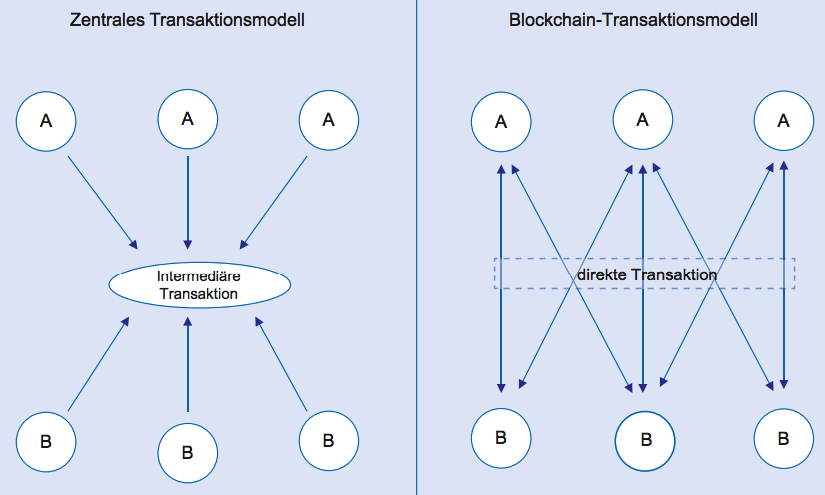
\includegraphics[width=1.0\linewidth]{pictures/change-in-transaction-model-blockchain}
	\caption[Transaktionsmodell Blockchain]{Transaktionsmodell Blockchain \textcolor{red}{QUELLE}}
	\label{fig:change-in-transaction-model-blockchain}
\end{figure}

Wird von einem der Teilnehmer eine Transaktion ausgelöst, wird diese nicht durch einen Intermediär sondern durch das Netzwerk erfasst und verarbeitet (Abbildung \ref{fig:change-in-transaction-model-blockchain}). Ein neuer \textit{Block} wird erschaffen und validiert wie es durch das Konsensprotokoll festgelegt wird. Dabei können solche \textit{Blockchain} Systeme unterschiedlich ausgeprägt sein. Dies zeigt sich zb. an der Art des Zugriffs, also wer darf Transaktionen lesen, wer darf sie schreiben. Außerdem kann der Mechanismus zur Konsensfindung je System anders sein.

% \citep{Abeyratne2016}
% \citep{Casino2019}

% \citep{Platzer2014}
% \citep{Narayanan2016}
% \citep{Burgwinkel2016}

% \citep{Gayvoronskaya2017}
% \citep{Vigna2017}
% \citep{JPMorgan2018}
% \citep{Buhl2017}
% \citep{Maull2017}
% \citep{Technik2018}
% \citep{Mitschele2018}
% \citep{Neugebauer2018}
% \citep{Min2018}


\subsubsection{Begriffliche Abgrenzung}

Die am häufigsten verwendeten Begriffe werden im Folgenden anhand eines Schichtenmodells (Abbildung \ref{fig:layer-model-blockchain}) erklärt und voneinander abgegrenzt. Jede Schicht wird in der Abbildung durch einen Balken dargestellt und ist unabhängig von den darüber liegenden Schichten. Von oben nach unten gelesen stehen die Schichten in einer \glqq ist enthalten in\grqq{} Beziehung zueinander. Entsprechend verlaufen die Schichten von einer konkreten Ausprägung zu einem abstrakten technologischen Konzept. Nachfolgend werden die einzelnen Schichten genauer erklärt.

\begin{figure}[H]
	\centering
	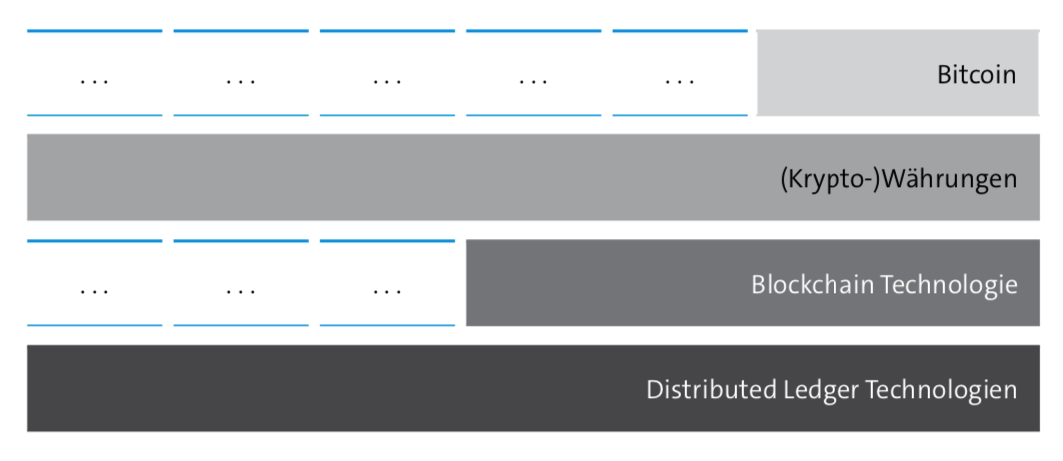
\includegraphics[width=1.0\linewidth]{pictures/layer-model-blockchain}
	\caption[Schichtenmodell \textit{Blockchain} Begriffe]{Schichtenmodell \textit{Blockchain} Begriffe \textcolor{red}{QUELLE}}
	\label{fig:layer-model-blockchain}
\end{figure}

\paragraph{Distributed Ledger}$~~$\\
Der \textit{Distributed Ledger} bildet die Basis des Schichtenmodells. Er ist im Grunde genommen ein klassisches Betandsbuch, das über einen Mechanismus verfügt, es auf alle teilnehmenden Parteien zu verteilen. \textit{Distributed Ledger} existieren bereits seit längerer Zeit und sind meist auf der technischen Basis einer verteilten Datenbank mit einer Logik auf Programm- oder Datenbankseite versehen, die aus der reinen Datenbank ein Bestandsbuch macht.

Distributed Ledger Technologie wird zunehmend synonym zum bisherigen Gebrauch von \textit{Blockchain} genutzt, um die Entwicklungen nach dem Bitcoin und den Kryptowährungen von eben diesen begrifflich abzugrenzen.

\paragraph{Blockchain-Technologie}$~~$\\
Die \textit{Blockchain} ist eine Form, einen \textit{Distributed Ledger} zu organisieren und zu implementieren. Auf die technische Implementierung der \textit{Blockchain} wird in den folgenden Kapiteln näher eingegangen; zur Begriffsbestimmung seien hier die grundlegenden Eigenschaften aufgezählt, die der \textit{Blockchain} in den letzten Jahren die steigende Aufmerksamkeit ermöglich haben:

\begin{itemize}
  \item Dezentralisiert
  \item Peer-to-Peer
  \item Transparenz und Anonymität
  \item Vertrauen
\end{itemize}

Blockchain gehört zu den bekanntesten Distributed-Ledger-Technologien. Aus diesem Grund wird die Bezeichnung Blockchain-Technologie in dieser Arbeit synonym für Distributed-Ledger-Technologien benutzt. Auf die technischen Eigenschaften von weiteren Ausprägungen der Distributed-Ledger-Technologien wird in dieser Arbeit daher nicht eingegangen.

\paragraph{Kryptowährungen}$~~$\\
Mit der \textit{Blockchain} als Basistechnologie lassen sich darauf aufbauende komplexe Systeme, wie z.B. Währungen abbilden. Wie in Kapitel \ref{blockchain-definition} erwähnt wurde die Blockchain-Technologie als erstes im Zusammenhang mit einer Kryptowährungen, dem Bitcoin, beschrieben. Die \textit{Blockchain} ist somit ein Nebenprodukt einer technischen Plattform, die eine kryptographische Währung erschuf und gleichzeitig ein System implementierte, um diese Währung zu nutzen und zu handeln.

Neben dem Bitcoin existiert eine Reihe weiterer Kryptowährungen, die sich zum Teil der dem Bitcoin zugrunde liegenden öffentlichen \textit{Blockchain} bedienen. Genannt seien hier z.B. Litecoin oder Dogecoin. Es existieren darüber hinaus Kryptowährungen, die eigene Blockchains zur Basis haben - zum Teil auf einer komplett eigenen technischen Implementierung. Vertreter hierfür sind z.B. Ethereum, Ripple oder Iota \citep[siehe auch][]{Buterin2014, carVertical, JPMorgan2018}.

\paragraph{Bitcoin}$~~$\\
Der Bitcoin ist die Kryptowährung, die auf der ursprünglichen \textit{Blockchain} gehandelt wird. Im Rahmen dieser Arbeit wird der Bitcoin und andere Kryptowährungen nicht weiter betrachtet.

\subsubsection{Arten von \textit{Blockchain}} \label{Arten-von-Blockchain}
Bei der Auswahl der Art einer \textit{Blockchain} trifft man auf zwei Widersprüche die nachfolgend kurz erläutert sind. Darauf folgt eine Betrachtung der Konfliktursachen und die sich daraus ableitenden Kategorien in die sich ein Blockchain System einordnen lässt.

\paragraph{Transparenz vs. Vertraulichkeit}$~~$\\
Verwendet man eine \textit{Blockchain} werden Besitzverhältnisse durch die Transaktionshistorie ermittelt. Dabei lässt sie eine \textit{Blockchain} mit einem öffentlichen Register vergleichen. Im Sinne der Übertragung von Eigentum sind Offenheit und Transparenz zwei wesentliche Eigenschaften der Blockchain. Durch diese Offenheit ist jeder Teilnehmer in der Lage alle Transaktionen einzusehen und auf Manipulationen zu prüfen.

Dieses Vorgehen steht im Gegensatz zur Vertraulichkeit, die in bestimmten Bereichen unabdingbar ist. Durch Vertraulichkeit werden Informationen wie die Transaktionsdaten oder deren Details (beteiligte Konten oder transferierte Menge) vor unbefugter Einsicht geschützt. Hierdurch entsteht der Widerspruch zwischen Transparenz auf der einen Seite und Anforderungen an die Vertraulichkeit auf der anderen Seite \citep{Drescher2017}.

\paragraph{Sicherheit vs. Geschwindigkeit}$~~$\\
Die Datenstruktur einer \textit{Blockchain} sichert die Transaktionshistorie vor Manipulationen und Fälschungen. Jeder neue \textit{Block} der in der \textit{Blockchain} gespeichert werden soll muss vom Netzwerk durch das Lösen einer kryptographischen Aufgabe erzeugt und der Datenstruktur hinzugefügt werden. Dadurch ist es ziemlich aufwendig die Transaktionshistorie nachträglich zu manipulieren oder zu fälschen. Durch diesen Sicherheitsmechanismus sinkt die Geschwindigkeit mit der ein \textit{Blockchain} Netzwerk neue Transaktionen verarbeiten kann. Moderne Applikationen erfordern Geschwindigkeit und Skalierbarkeit was im direkten Kontrast zum erwähnten Sicherheitskonzept einer \textit{Blockchain} steht \citep{Drescher2017}.

\paragraph{Ursachen der Konflikte}$~~$\\
Zwei grundlegende Operationen eines \textit{Blockchain} Netzwerks sind Ursache für die beiden beschriebenen Widersprüche - Schreiben und Lesen von Transaktionsdaten. Der Konflikt zwischen Transparenz und Vertraulichkeit ist auf die Lese-Operationen einer \textit{Blockchain} zurückzuführen. Je offener die Leseberechtigungen einer \textit{Blockchain} sind, desto höher ist die Transparenz und desto niedriger ist die Vertraulichkeit der Transaktionsdaten. Die Schreib-Operationen sind für den Widerspruch zwischen Sicherheit und Geschwindigkeit verantwortlich. Je restriktiver die Berechtigungen zum Schreiben innerhalb des \textit{Blockchain} Netzwerks sind, desto höher ist die Geschwindigkeit mit der Transaktionen verarbeitet werden können. In Tabelle \ref{tab:technical-restricts-blockchain} werden die technischen Beschränkungen, der Widerspruch und die Operation innerhalb der \textit{Blockchain} zusammengefasst \citep{Drescher2017}.

\begin{table}[H]
	\begin{tabular}{@{}lll@{}}
		\toprule
		\textbf{Beschränkung} & \textbf{Widerspruch}            & \textbf{Blockchain Operation} \\
		\midrule
		Keine Vertraulichkeit & Transparenz vs. Vertraulichkeit & Transaktionshistorie lesen    \\ \addlinespace
		Skalierbarkeit        & Sicherheit vs. Geschwindigkeit  & Transaktionen schreiben       \\
		\bottomrule
	\end{tabular}
	\caption{Technische Beschränkungen der \textit{Blockchain} und ihre Ursachen}
    \label{tab:technical-restricts-blockchain}
\end{table}

\paragraph{Public vs. Private}$~~$\\
Betrachtet man die Berechtigungen zum Lesen innerhalb eines \textit{Blockchain} Netzwerks in der einfachsten Form muss das System zwischen Transparenz und Vertraulichkeit entscheiden. Entweder es werden allen Teilnehmern Leseberechtigungen zugeteilt oder nur einer ausgewählten Gruppe von Teilnehmern. Anhand des Kriterium, welcher Teilnehmer im Netzwerk neue Transaktionen erstellen und die Historie lesen kann, lässt sich eine \textit{Blockchain} als öffentliche oder private \textit{Blockchain} charakterisieren \citep{Drescher2017}.

\paragraph{Permissioned vs. Permissionless}$~~$\\
Die Schreibrechte bestimmen für ein \textit{Blockchain} Netzwerk den Grad der Skalierbarkeit. Werden Schreibrechte in ihrer einfachsten Form zugeteilt und alle Teilnehmer sind berechtigt Schreib-Operationen auszuführen, erhöht sich der Arbeitsaufwand je Teilnehmer der zur Berechnung nötigt wird. Dies ist für die Sicherheit des Netzwerk positiv, wirkt sich aber negativ auf die Geschwindigkeit aus. Durch die Geschwindigkeit wird das Netzwerk in der Skalierbarkeit beschränkt. Teilt man hingegen nur einer Gruppe von Teilnehmern Schreibrechte zu, ist der Arbeitsaufwand im Vergleich niedrig. Hierdurch kann das Netzwerk Transaktionen vergleichsweise schnell verarbeiten und ist dadurch selbst skalierbarer \citep{Drescher2017}.

\begin{table}[H]
	\resizebox{\textwidth}{!}{%
	\begin{tabular}{@{}lll@{}}
	\toprule
								& \textbf{Permissionless}                                                                                                               & \textbf{Permissioned}                                                                                                                    \\
	\midrule
	\textbf{Public}             & \begin{tabular}[c]{@{}l@{}}Bitcoin, Ethereum, IOTA\\ \\ Jeder kann validieren\\ Jeder kann teilnehmen\end{tabular}                    & \begin{tabular}[c]{@{}l@{}}Ethereum 2.0\\ \\ Ausgewählte Gruppe kann validieren\\ Jeder kann teilnehmen\end{tabular}                     \\
	\midrule
	\textbf{Consortium/Private} & \begin{tabular}[c]{@{}l@{}}Interplanetary Database(IPDB)\\ \\ Jeder kann validieren\\ Ausgewählte Gruppe kann teilnehmen\end{tabular} & \begin{tabular}[c]{@{}l@{}}Hyperledger, Quorum\\ \\ Ausgewählte Gruppe kann validieren\\ Ausgewählte Gruppe kann teilnehmen\end{tabular} \\
	\bottomrule
	\end{tabular}%
	}
	\caption{Arten von Blockchain Netzwerken (eigene Darstellung)}
	\label{tab:types-of-blockchain-networks}
\end{table}

\noindent
Alle zuvor beschriebenen Eigenschaft einer Blockchain ermöglichen es eine Matrix mit zwei Dimensionen zu modellieren in die sich nahezu sämtliche Blockchain Lösungen einordnen lassen. Ausgenommen sind etwaige Mischformen, die für sehr spezielle Anwendungsfälle konzipiert wurden und sich beispielsweise aus einer Kombination einer öffentlichen und konsortialen Blockchain zusammensetzen. Tabelle \ref{tab:types-of-blockchain-networks} zeigt diese Matrix. Die vertikale Achse beschreibt in diesem Fall die Anonymität der Teilnehmer. Diese reicht von vollständiger Anonymität\footnote{Anonymität meint hier eine Pseudo-Anonymität, da aus technischer Sicht mit einigem Aufwand der Teilnehmen klar identifiziert werden kann.} bis zur Offenlegung und direkten Verknüpfung zwischen einem Teilnehmer des Netzwerks und einer Entität (Person, Maschine oder Unternehmen) in der realen Welt. Auf der horizontalen Achse wird das Vertrauen in die Validatoren abgebildet. Konkret können entweder alle Teilnehmer auch als Validatoren auftreten (Permissionless) oder es wird eine Gruppe von Teilnehmern zum validieren von Transaktionen gebildet, die definierte Anforderungen erfüllen (Permissioned). An den Schnittpunkten der Zeilen und Spalten wurden Beispiele für Implementationen der jeweiligen Kombination eingefügt.

%\subsubsection{Technologischer Hintegrund}
%Eine \textit{Blockchain} operiert auf einem \textit{Peer-to-Peer} Netzwerk in welchem jeder \textit{Knoten} eine exakte Kopie der Transaktionshistorie vorhält. Eine \textit{Blockchain} ist somit eine verteilte Datenbank, die eine kontinuierliche Liste von Transaktionen speichert und durch kryptographische Mechanismen vor Manipulation schützt. Transaktionen werden anhand eines Konsensusprotokolls validiert und zur Liste der Transaktionen hinzugefügt \citep{Nakamoto2009}.

\subsubsection{Peer-to-Peer Netzwerke}
Ein \textit{Peer-to-Peer} Netzwerk ist der Gegensatz zum klassischen \textit{Client-Server-Modell}, bei dem ein \textit{Server} einen Dienst zur Verfügung stellt und ein oder mehrere \textit{Clients} diesen Dienst abrufen und nutzen. Bei einem \textit{Peer-to-Peer} Netz sind alle Teilnehmer, die sog. \textit{Peers}, gleichberechtigt und können Dienste anbieten und auch konsumieren. \textit{Peer-to-Peer} Netzwerke operieren als \textit{Overlay-Netze}\footnote{Ein \textit{Overlay-Netz} baut auf ein bestehendes Netz (\textit{Underlay Netz}) auf. Es kann mit eigenen Protokollen arbeiten und selbst als \textit{Underlay Netz} fungieren.\citep{Andersen2001}} auf dem Internet. Einige der häufigsten Eigenschaften von \textit{Peer-to-Peer} Netzwerken sind nach \citet{Steinmetz2005}:

\begin{itemize}
  \item Heterogenität zwischen den \textit{Peers} in Bezug auf Bandbreite, Rechenkraft und Speichergröße
  \item Qualität einzelner \textit{Peers} in Form von Verfügbarkeit und Verbindungsstärke lässt sich nicht voraussetzen
  \item Client-Server-Funktionalität wird für \textit{Peers} ermöglicht, um Dienste und Ressourcen anzubieten und zu konsumieren
  \item Austausch von Diensten und Ressourcen unter allen \textit{Peers} gewährleistet
  \item Bereitstellung von Such-Funktionen durch ein zusätzliches \textit{Overlay-Netz}
  \item Autonomie der \textit{Peers} in punkto Ressourcenbereitstellung
  \item Das \textit{Peer-to-Peer} Netzwerk organisiert sich selbst und nicht durch Dritte
\end{itemize}

\subsubsection{Kryptografisches Hashing}
Kryptografisches Hashing gehört zu einem der wichtigsten Instrumente der Kryptografie und bildet einen eigenen Teilbereich der Kryptografie. Mit einer kryptografischen Hash-Funktion lässt sich aus einem beliebig langen Wort (oder Datensatz) eine Zeichenkette mit fixer Stellenanzahl generieren. Die jeweilige Ausgabelänge wird in Bit angegeben. Formal ist eine Hash-Funktion definiert als

\begin{equation}
	f:\left \{ 0,1 \right \}^{*} \mapsto \left \{ 0,1 \right \}^{n}
\end{equation}

Das Ergebnis wird als digitaler Fingerabdruck bezeichnet. Die Generierung des Hash-Werts ist nicht zwingend kryptografisch, denn nicht jede Hash-Funktion erfüllt alle Anforderungen einer kryptografischen Hash-Funktion \citep{Menezes1997, Diffie1976}. Dabei gilt, eine kryptografische Hash-Funktion muss folgende Kriterien erfüllen:

\begin{itemize}
	\item Eindeutigkeit
	\item Reversibilität
	\item Kollisionsresistenz
\end{itemize}

Mit der Eindeutigkeit ist gegeben, dass ein bestimmter Eingabewert immer zum selben Ausgabewert führt. Reversibilität beschreibt die Eigenschaft einer Hash-Funktion, das der Ausgabewert nicht in den ursprünglichen Eingabewert zurückberechnet werden kann. Die Kollisionsresistenz sorgt dafür, dass zwei unterschiedliche Eingabewerte nicht den gleichen Ausgabewert erzeugen. Abbildung \ref{fig:schema-hash-function} zeigt schematisch die Funktionsweise einer kryptografischen Hash-Funktion. Der Eingabewert, hier Urbild, wird durch die kryptografische Hash-Funktion in einen Ausgabewert (Hash-Wert) fester Länge transformiert.

\begin{figure}[H]
	\centering
	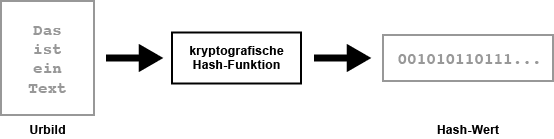
\includegraphics[width=1.0\linewidth]{pictures/schema-hash-function}
	\caption[Funktionsweise einer kryptografischen Hash-Funktion]{Funktionsweise einer kryptografischen Hash-Funktion \textcolor{red}{QUELLE Elektronik Kompendium}}
	\label{fig:schema-hash-function}
\end{figure}

\subsubsection{Signierte Transaktionen durch Public-Key-Infrastruktur}
Wird eine Transaktion von einem Teilnehmer erstellt und soll durch das Netzwerk validiert werden kommen digitale Signaturen zum Einsatz. Digitale Signaturen gehören zur asymmetrischen Kryptographie und werden dazu verwendet die Urheberschaft und Integrität einer Nachricht oder, im Falle der Blockchain, einer Transaktion zu prüfen.\citep{Beutelspacher2010, Menezes1997}

\begin{figure}[H]
	\centering
	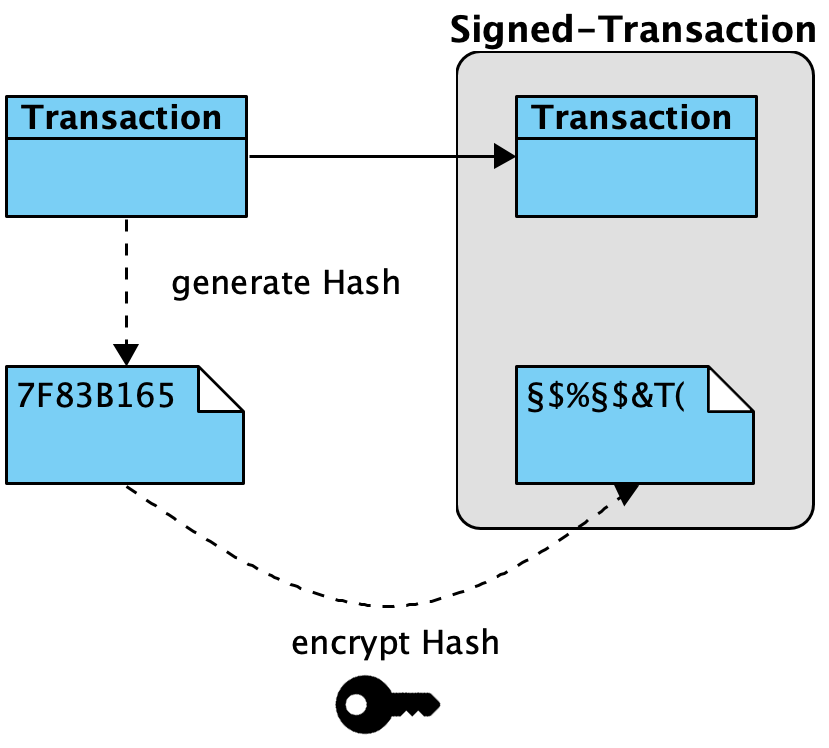
\includegraphics[width=0.7\linewidth]{pictures/digital-signatures-create}
	\caption[Erstellen einer digitalen Signatur]{Schematische Darstellung für das Erstellen einer digitalen Signatur (in Anlehnung an \citet{Drescher2017})}
	\label{fig:digital-signatures-create}
\end{figure}

In Abbildung \ref{fig:digital-signatures-create} wird das digitale Signieren einer Transaktion verdeutlicht. Der Prozess startet oben links in der Abbildung mit einer Transaktion. Durch Anwendung einer kryptographischen Hashfunktion wird ein Hash gebildet. Dieser Hashwert wird anschließend mit dem privaten Schlüssel des Erstellers verschlüsselt. Dieser verschlüsselte Hashwert ist die digitale Signatur und zusammen mit der Transaktion bilden sie die digital signierte Transaktion. Durch die Verwendung der \ac{pki} ist die digitale Signatur auf zwei Arten einzigartig. Zum einen kann der Ersteller der Signatur eindeutig zugeordnet werden und zum anderen wird die Integrität der Transaktion sichergestellt \citep{Drescher2017}.

\begin{figure}[H]
	\centering
	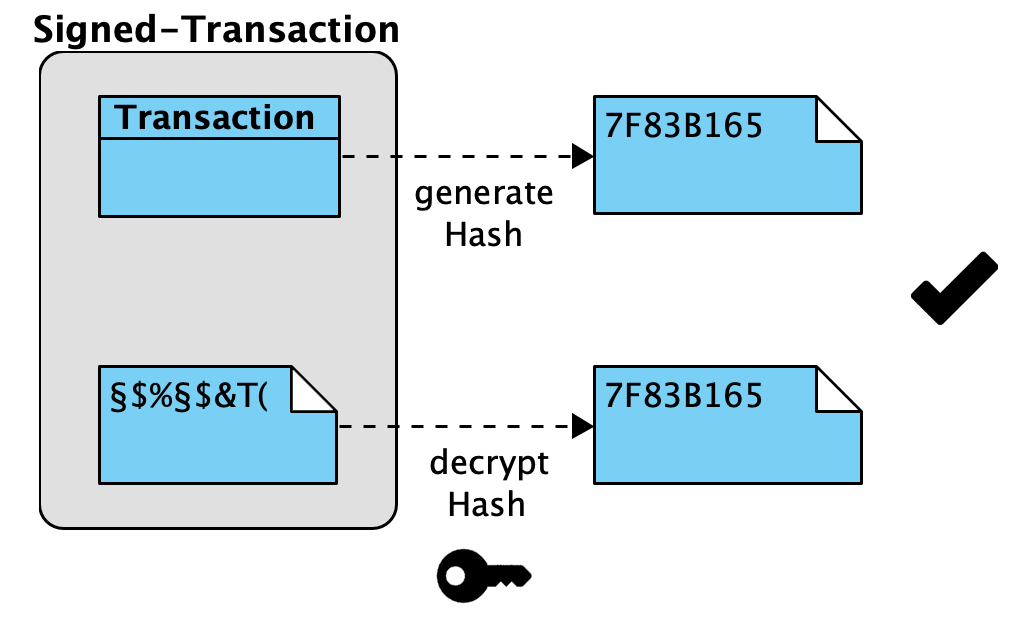
\includegraphics[width=0.7\linewidth]{pictures/digital-signatures-validate-positive}
	\caption[Prüfen einer digitalen Signatur]{Erfolgreiche Prüfung einer digitalen Signatur (in Anlehnung an \citet{Drescher2017})}
	\label{fig:digital-signatures-validate-positive}
\end{figure}

Soll eine signierte Transaktion vom Netzwerk verarbeitet und erfolgreich verbucht werden müssen zwei Eigenschaften erfüllt sein. Die Urheberschaft muss eindeutig zuzuordnen sein und die Integrität der Transaktion darf nicht verletzt worden sein. Dazu wird wie in Abbildung \ref{fig:digital-signatures-validate-positive} zuerst mit dem öffentlichen Schlüssel des Absenders die digitale Signatur entschlüsselt. Gelingt dies, ist sichergestellt das der Ersteller der digitalen Signatur eindeutig über die \ac{pki} zugeordnet werden kann. Im zweiten Schritt wird aus der Transaktion der Hashwert gebildet und mit der entschlüsselten digitalen Signatur verglichen. Sind beide Werte gleich ist garantiert, dass die Transaktion auf dem Weg der Übermittlung nicht manipuliert wurde \citep{Drescher2017}.

Stellt sich bei der Überprüfung der signierten Transaktion heraus, dass die Hashwerte nicht übereinstimmen können zwei Gründe dafür verantwortlich sein. Entweder wurde die eigentliche Transaktion während der Übermittlung von einem Angreifer manipuliert oder die Transaktion wurde nicht vom vermeintlichen Teilnehmer des Netzwerks autorisiert \citep{Drescher2017}. Abbildung \ref{fig:digital-signatures-validate-negative} zeigt schematisch diese Situation.

\begin{figure}[H]
	\centering
	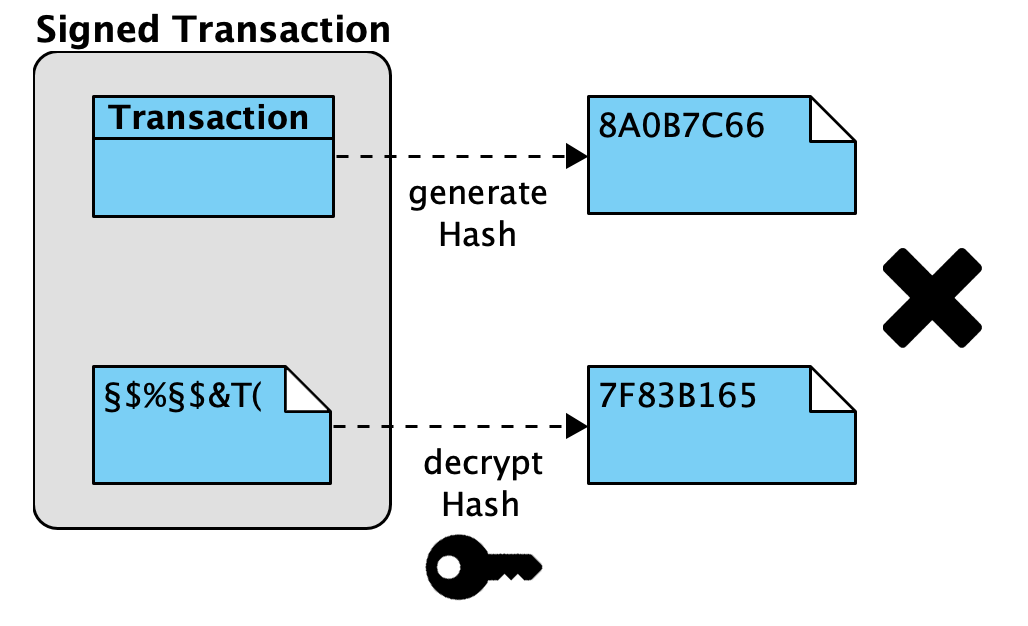
\includegraphics[width=0.8\linewidth]{pictures/digital-signatures-validate-negative}
	\caption[Manipulationerkennung durch digitale Signaturen]{Erkennung von Manipulation anhand der digitalen Signatur (in Anlehnung an \citet{Drescher2017})}
	\label{fig:digital-signatures-validate-negative}
\end{figure}

\subsubsection{Konsensmechanismen}
Es gibt hauptsächlich zwei Kategorien von Konsensmechanismen:

\begin{itemize}
	\item Lotterie-basiert
	\item Byzantinische Fehlervereinbarung
\end{itemize}

Die erste Kategorie wird auch Nakamoto-Konsens genannt nach dem Pseudonym des Bitcoin Erfinders Satoshi Nakamoto. Der Konsensmechanismus wählt den Prüfer, d.h. den Knoten, der entscheidet, welcher der nächste Block ist, der an die Blockchain angehangen wird. Dabei ist die Wahl eine Lotterieziehung. Der Gewinner ist der Validierer. Jeder neue Block erfordert auch eine neue Ziehung eines Validierers. Die Auswahl durch eine Lotterie reduziert die Wahrscheinlichkeit, dass ein kompromittierter Knoten einen gefälschten Block validiert. Hierbei folgt die Lotterie keiner gleichwertigen Verteilung. Jeder Mechanismus definiert seine eigene Wahrscheinlichkeitsverteilung anhand eine bestimmte Eigenschaft des Gewinners bevorzugt wird. So besitzt jeder Lotterie-basierte Konsensmechanismus ein anderes Vertrauensmodell. Bitcoin beispielsweise verwendet den bekanntesten Mechanismus - \acf{pow}. Daneben gibt es wie beschrieben noch einige andere Mechanismen wie \acf{pos}, \acf{posp} oder \acf{poet}.

\acf{bft}-Systeme bilden die Basis für Mechanismen der zweiten Kategorie. \ac{bft}-Systeme sind so konzipiert, dass sie auch bei Ausfall einiger Teilnehmer des Netzwerks weiterhin funktionieren. Dabei kann der Ausfall unfreiwillig (z.B. ein teilnehmender Knoten ist außer Betrieb) oder freiwillig (z.B. ein Angreifer kontrolliert den fehlerhaften Knoten) sein. \ac{bft}-Systeme verwenden Abstimmungsmechanismen, um einen Konsens herstellen zu können. Der verwendete Mechanismus legt das Vertrauensmodell fest. Der \acf{pbft} Mechanismus ist der bekannteste Mechanismus dieser Kategorie.
Außerdem sind hybride Konsensmechanismen möglich die eine Mischung aus Lotterie und \ac{bft} darstellen. Nachfolgend sollen die beiden meist verwendeten Konsensmechanismen kurz erläutert werden.

\paragraph{Proof-of-Work}$~~$\\
Das Konzept des \acf{pow} existierte schon vor der ersten Blockchain Applikation (Bitcoin). Die erste moderne Anwendung wurde 1996 von Adam Back unter dem Namen \glqq Hashcash\grqq{} eingereicht. Diese Anwendung hat auf Grundlage des SHA265-Algorithmus einen \ac{pow} Mechanismus eingesetzt um E-Mail Spam zu verhindern \citep{Back2002}.

Der Mechanismus des \ac{pow} kann relativ simpel beschrieben werden. Es ist die Tatsache, dass ein Teilnehmer des Netzwerks allen anderen Teilnehmern das Ergebnis der von ihm durchgeführten Berechnungen vorlegt. Die durchzuführenden Operationen sind an sich nicht kompliziert, allerdings müssen sie so oft durchgeführt werden, dass der Teilnemer eine erhebliche Rechenleistung dafür aufbringen muss. Daher spricht man von \glqq Proof-of-Work\grqq{}, da der Teilnehmer mit einem korrekten Ergebnis einen Nachweis seiner geleisteten Arbeit gibt. Konkret muss der Teilnehmer ein Ergebnis finden, das mit einer  bestimmten Anzahl an führenden Nullen beginnt. Je größer die Anzahl der führenden Nullen ist, desto schwierieger ist es für den Teilnehmer ein valides Ergebnis zu finden. Die Anzahl der Nullen bzw. die Schwierigkeit wird an die Anzahl der Teilnehmer und ihrer Rechenleistung im Netzwerk angepasst, sodass ein neues Ergebnis in festen Intervallen gefunden werden kann.\footnote{Im Bitcoin Blockchain Netzwerk wird die Schwierigkeit dauerhaft so angepasst, dass nur alle 10 Minuten ein neuer Block berechnet werden kann.} Für die Berechnung des Ergebnisses fügt der Teilnehmer zu den eigentlichen Transaktionsdaten eine sogenannte \glqq Nonce\grqq{} hinzu. Aus diesen Daten versucht der Teilnehmer das Ergebnis zu berechnen mit der entsprechenden Anzahl an führenden Nullen. Bei jeder Runde wird die \glqq Nonce\grqq{} verändert. Dies wird solange durchgeführt bist das Ergebnis zur aktuellen Schwierigkeit im Netzwerk passt.

\paragraph{Practical Byzantine Fault Tolerance}$~~$\\
Das \ac{pbft}-Modell konzentriert sich in erster Linie auf die Bereitstellung einer Zustandsmaschine, die byzantinische Fehler (kompromittierte Knoten oder Netzwerkteilnehmer) toleriert. Dies geschiet durch die Annahme, dass es unabhängige Knotenausfälle und manipulierte Nachrichten gibt. Der Algorithmus wurde für den Einsatz in asynchronen Systemen konzipiert und optimiert auf hohe Performance. Im Wesentlichen sind alle Knoten im \ac{pbft}-Modell in Reihe angeordnet, wobei ein Knoten als Primärknoten und die restlichen Knoten als Backupknoten bezeichnet werden. Alle Knoten innerhalb des Systems kommunizieren untereinander mit dem Ziel einen einheitlichen Zustand des Systems zu finden. Die Knoten müssen dabei nachweisen, das eine Nachricht von ihnen stammt und das diese Nachricht während der Übertragung nicht manipuliert wurde \citep{Tuan2017}.

Damit das \ac{pbft}-Modell funktioniert, wird davon ausgegangen, dass die Anzahl der kompromittierten Knoten im Netzwerk nicht größer oder gleich \nicefrac{1}{3} der Gesamtanzahl an Knoten im Netzwerk ist. Je mehr Knoten das Netzwerk bilden, desto mathematisch unwahrscheinlicher ist es, dass eine Anzahl von Knoten die sich \nicefrac{1}{3} der Gesamtknotenanzahl nähert kompromittiert ist.

Jede Runde des \ac{pbft}-Konsens, genannt \textit{Views}, besteht aus 4 Phasen. Das Modell folgt dabei eher dem Format \glqq Kommandant und Offiziere\grqq{} durch die Anwesenheit des Primärknotens. Beim byzantinischen Generalsproblem sind alle Generäle gleichwertig, was hier nicht der Fall ist. Die Phasen des \ac{pbft}-Konsens sehen wie folgt aus.

\begin{enumerate}
	\item Ein Client sendet eine Anfrage an den Primärknoten, um eine Serviceoperation durchzuführen.
	\item Der Primärknoten sendet die Anfrage an alle Backupknoten.
	\item Die Knoten führen die Anfrage aus und senden eine Antwort an den Client.
	\item Der Client erwartet \(3f + 1\) Antworten von verschiedenen Knoten mit dem gleichen Ergebnis.\footnote{Mit \(f\) ist die Anzahl an tollerierbaren kompromittierten Knoten gemeint.} Das Ergebnis ist das Ergebnis der Serviceoperation.
\end{enumerate}

Alle Knoten müssen die Anforderung erfüllen deterministisch zu operieren und im gleichen Zustand mit der Operation zu beginnen. Das Endergebnis ist, das sich alle nicht-kompromittierten Knoten auf die Reihenfolge der Datensätze einigen und dies geschlossen akzeptieren oder ablehnen.

Der Primärknoten wird in jeder \textit{View} nach dem Round-Robin Verfahren ausgewählt und kann auch ausgetauscht wurde durch eine Erweiterung des Modells. Ein Austausch kann durchgeführt werden, wenn der Primärknoten die Anfrage nicht innerhalb eines bestimmten Zeitlimits an die Backupknoten weiterleitet.

\textcolor{red}{Quellen ergänzen!}


\newpage

\section{Lösungskonzept} \label{solution-concept}
Dieses Kapitel soll aufzeigen mit welcher konkreten Ausprägung der Blockchain Techologie der gewählte Use-Case realisiert werden kann. Dazu wird im ersten Schritt eine SWOT-Analyse zur Blockchain Technologie allgemein durchgeführt und die Ergebnise beschrieben. In Schritt zwei kommt eine Nutzwertanalyse zum Einsatz anhand welcher ermittelt wird welche Ausprägung der Technologie sich zur Umsetzung bestmöglichst eignet.

\subsection{SWOT-Analyse der \textit{Blockchain-Technologie}} \label{swot-analyse}
Durch die Vielzahl an unterschiedlichen Use-Cases die mittels der Blockchain Technologie umgesetzt werden ist es nötig für den spezifischen Use-Case der Chargenrückverfolgung die Technologie einer SWOT-Analyse zu unterziehen. Hierdurch wird gewährleistet, dass die Technologie für den Use-Case überhaupt geeignet ist. Im folgenden werden daher aus interner Sicht die Stärken und Schwächen gegenübergestellt, sowie die dadurch möglichen externen Chancen und Risiken diskutiert. Abbildung \ref{fig:blockchain-technology-swot-analysis} zeigt eine schematische Sicht der SWOT-Analyse.

\begin{figure}[H]
	\centering
	
\includegraphics[width=1\linewidth]{pictures/blockchain-technology-swot-analysis}
	\caption[Blockchain Technologie SWOT Analyse]{Blockchain Technologie SWOT Analyse (eigene Darstellung)}
	\label{fig:blockchain-technology-swot-analysis}
\end{figure}

\subsubsection{Stärken}
\paragraph{Manipulationsicherheit}
Eine der Schlüsselstärken der Technologie ist, dass sie eine Manipulation von Datensätzen direkt erkennbar macht durch die Art und Weise wie Transaktionen gespeichert und verknüpft werden.

\paragraph{Schutz der Privatsphäre}
Durch eine Implementierung eines Berechtigungskonzepts können Teilnehmer des Netzwerks eigenständig definieren wer auf die Daten zugreifen kann, für welchen Zweck und für welchen Zeitraum. Diese Regeln werden in Smart Contracts programmatisch abgebildet und bei jeder Ausführung geprüft. So lassen sich beispielsweise komplexe Berechtigungsstrukturen direkt innerhalb des Netzwerks abbilden ohne dazu eine zusätzliche Abstraktionsebene einführen zu müssen. 

\paragraph{Effizienzsteigerung}
Zusätzlich zur Manipulationsicherheit und dem Schutz der Privatsphäre bietet die Blockchain Technologie die Möglichkeit der Effizienzsteigerung für Geschäftsprozesse. Durch den Einsatz von Kryptographie können zwei Parteien vertrauensvoll miteinander interagieren. Eine gesonderte Prüfung der Transaktionen entfällt hierbei, da sie durch Smart Contracts bereits geprüft wurde. Hierdurch entsteht ein Einsparungspotential bzw. eine Effizienzsteigerung.

\subsubsection{Schwächen}
\paragraph{Mangelnde Kontrolle}
In der Theorie sind Blockchain Lösungen dezentralisiert und selbstverwaltend \citep[siehe auch][]{Nakamoto2009} in der Praxis zeigt sich jedoch, dass der Betrieb eines solchen Systems maßgeblich unter der Kontrolle einer Gruppe von Entwicklern bzw. einer eigens dafür gegründeten Organisation steht.

\paragraph{Fehlender Kontext}
Eine weitere Schwäche ist das Fehlen eines Mechanismus, um Datensätze in der Kette zurück in den Geschäftskontext ihrer Erstellung zu verknüpfen. Dies kann es schwierig machen, sich auf Blockchain-Datensätze als Nachweis für Geschäftsvorgänge zu verlassen.

Betrachten Sie eine Blockchain-Lösung, wie sie in Schweden und Brasilien erprobt wurde, bei der Landtransfers und Millionen anderer Transaktionen auf einer öffentlichen Blockchain erfasst wurden. Wie wäre es möglich, den auf der Blockchain aufgezeichneten Hash abzurufen, der einem bestimmten Landtitel zugeordnet ist, wenn es keine Möglichkeit gibt, die Transaktion mit ihrem Geschäftskontext zu verknüpfen? Wie wäre es möglich, E-Discovery-Aufträge zu erfüllen?

\paragraph{Verletzung des Datenschutzes}
Gesetze zur Datenlokalisierung können sich aus Gesetzen und Vorschriften ergeben, die die Aufbewahrung von Dokumenten in einem Geschäftsgebäude vorschreiben, oder aus Gesetzen, die sich mit Datenschutz und Privatsphäre in Bezug auf Technologie befassen. Im europäischen Kontext ist ein Beispiel die \ac{dsgvo}, die Anforderungen an die Verarbeitung personenbezogener Daten stellt. Für Länder, die sich auf die Speicherung von Elementen ihrer öffentlichen Aufzeichnungen in einer Blockchain verlassen, die nicht vollständig in ihrer Hoheitsgewalt operiert, ist es notwendig zu prüfen, ob das System den Gesetzen und Vorschriften zur Datenlokalisierung und zum Datenschutz entspricht.

\subsubsection{Chancen}
\paragraph{Neue Geschäftsmodelle}
Überall dort wo zur Zeit noch Intermediäre eingesetzt werden zur Abwicklung von Transaktionen zwischen zwei oder mehreren Parteien kann die Blockchain Technologie eingesetzt werden. Mit dem Einsatz von Smart Contracts können Verträge auf der Blockchain abgebildet und mit Hilfe von Algorithmen dezentral über das Netzwerk ausgeführt werden. Es ist nicht notwendig das Intermediäre für die Ausführung und Gestaltung der Verträge von den Vertragsparteien beauftragt werden. Die Erfüllung des Vertrags wird ebenfalls vollständig über die Blockchain kontrolliert und automatisch verwaltet. Unternehmen die als einziges Geschäftsmodell die Vermittlung und Bereitstellung einer Plattform für Anbieter und Kunde haben, also rein zur Abwicklung von Transaktionen dienen, können durch den Einsatz einer Blockchain obsolet werden. Das selbe Prinzip lässt sich auch auf das Lieferketten Management anwenden. 

\paragraph{Komplexität reduzieren}
Der Nachweis einer Charge eines beliebigen Lebensmittels vom Hersteller bis zum Urerzeuger aller verwendeter Bestandteile kann weit über 200 Papierdokumente von allen beteiligten Teilnehmern der Lieferkette erzeugen. Zahlreiche Amtstellen benötigen diese Dokumente für Nachweispflichten in Bezug auf Hygiene- und Gesundheitsvorschriften. Streckt sich die Lieferkette über mehrere Länder oder sogar Kontinente aus müssen in den meisten Fällen für Zollbehörden ebenfalls Originaldokumente zum Herkunftsnachweis gefordert. Kleinste Mängel an den Dokumente können zu Verzögerungen führen und Chargen die sich im Transit befinden verderben lassen oder die Zahlungen verlangsamen. Mit einer Blockchain kann hier die Komplexität des Prozesses vermindert werden. Jedesmal wenn ein Dokument mehreren Teilnehmern zur Verfügung stehen muss, ermöglicht die Blockchain durch das Hinzufügen eines Datensatzes das sämtliche Aktualisierungen des Dokuments in Echtzeit bereitstehen und die Gültigkeit und Integrität durch das Netzwerk abgesichert sind. Dies kann zu Zeit- und Kosteneinsparungen führen.

\subsubsection{Risiken}
\paragraph{Niedrige Verbreitung}
Im Lieferkettenmanagement sind alle Teilnehmer in einem Netzwerk organisiert. Je optimierter dieses Netzwerk ist desto besser kann es in seiner Gesamtheit performen. Entscheiden sich einige Teilnehmer dafür die Blockchain Technologie einzusetzen und einige Teilnehmer nicht so entsteht ein klassischer Systembruch wodurch in diesem Fall die Effizienz der Blockchain sinkt. Wenn beispielsweise die Urerzeuger nicht an dem Blockchain Netzwerk teilnehmen, kann ein vollständiger Nachweis allein über die Blockchain vom Hersteller nicht erbracht werden. Die Vertrauenskette endet an dem Punkt an dem ein virtuelles Gut, was in der Blockchain abgebildet ist, Produktionschritte durchläuft die nicht über die Blockchain abgewickelt werden. 

\paragraph{Angriffe und Fremdeinwirkung}
Wie auch andere IT Landschaften ist ein Blockchain Netzwerk nicht vollkommen vor Angriffen von außen oder innen geschützt. Sicherheitslücken in der verwendeten Plattform der Blockchain oder logische Fehlkonstrukture in Smart Contracts können ein Netzwerk beschädigen oder es sogar komplett stilllegen. Ein möglicher realer Wertverlust für die Teilnehmer des Netzwerk ist in einem solchen Fall kaum zu umgehen. Ebenfalls kann die Vertrauenskette komprimitiert werden durch bewusste Falscheingabe von Informationen und Metadaten. 

\subsection{Nutzwertanalyse}
Die Nutzwertanalyse unterstützt die Auswahl einer Alternative. Sie wird in diesem Kontext eingesetzt um verschiedene Entscheidungsvarianten miteinander vergleichen zu können. Neben den Entscheidungsvarianten werden Bewertungskriterien definiert und mit dem paarweisen Vergleich priorisiert. Nachdem die Varianten bewertet worden sind kann ein Ergebnis aus der Analysetabelle gelesen werden.

\subsubsection{Entscheidungsvarianten}
Als Entscheidungsvarianten wurden im Rahmen dieser Arbeit vier potentielle Kandidaten ausgewählt - Ethereum, Hyperledger Fabric, IOTA sowie Quorum. Nachfolgend soll eine kurze Beschreibung dazu dienen alle Kandidaten im Kontext der Blockchain Technologie vorzustellen.

\paragraph{Ethereum}
Ethereum war die erste Ausprägung der Blockchain Technologie in der Smart Contracts realisiert wurden. Aus diesem Grund wurde Ethereum als erste Option zur Umsetzung einer Supply Chain Lösung in betracht gezogen, denn ohne die Möglichkeit der programmatischen Ausführung von Geschäftslogik lassen sich moderne IT-gestützte Geschäftsprozesse gar nicht erst mit einem Blockchain System abbilden. Die Bitcoin Blockchain besitzt in ihrer ursprünglichen Form beispielsweise keine Unterstützung für Smart Contracts und wurde daher auch direkt als möglicher Kandidat ausgeschlossen. Ethereum ist eine Open Source Lösung. Das Ethereum Netzwerk hat keine Zulassungsbeschränkungen und ist öffentlich, d.h. jeder kann am Netzwerk teilnehmen und auch selber Transaktionen anderer Teilnehmer validieren. Hierdurch ist ein hoher grad an Dezentralisierung und Transparenz gegeben, da keine einzelne Entität das Netzwerk und den Validierungsprozess kontrolliert. Ebenso unterstützt diese Offenheit die Ausfallsicherheit des gesamten Netzwerk sowieso einen gewissen Schutz vor Angriffen aus dem Netzwerk selbst. Ethereum verwendet zur Programmierung von Smart Contracts die Sprache Solidity.

\paragraph{Hyperledger Fabric}
Hyperledger Fabric ist, wie Ethereum, eine Open Source Lö\-sung. Die Implementierung der Blockchain Technologie wurde Ursprünglich von IBM entwickelt und dann an die Linux Foundation übergeben, welche es dann der Öffentlichkeit frei zur Verfügung stellte. Hyperledger Fabric ist kein fertiges Blockchain Netzwerk welches für einen bestimmten Anwendungsfall konzipiert wurde. Es ist ein Framework um Business Netzwerke und deren Transaktionen in einer einheitlichen Modellierungssprache zu erfassen und umzusetzen. Mit Hyperledger Fabric modellierte Netzwerke sind permissioned und private bzw. in konsortial Form aufgesetzt. Das bedeutet nur ein ausgewählter Kreis an Parteien darf an dem Netzwerk teilnehmen und die Validierung von Transaktionen wird von einer ausgewählten Gruppe von Teilnehmern durchgeführt. Hierdurch weisen Hyperledger Fabric Blockchain Netzwerke eine wesentlich höhere Durchsatzrate für Transaktionen auf als Ethereum, außerdem skaliert ein solches Netzwerk besser, da die Validierungsdauer nicht zwingend mit der Anzahl der Netzwerkteilnehmer ansteigt.

\paragraph{IOTA}
IOTA wurde entwickelt für eine sichere Kommunikation und Zahlungen im Machine-to-Machine Bereich und dem Internet der Dinge. Das IOTA Netzwerk ist ähnlich wie Ethereum permissionless und public. Im Gegensatz zu Lösungen wie Ethereum oder Hyperledger Fabric verwendet IOTA keine Blockchain als Datenstrukur sondern den sogenannten \glqq Tangle\grqq{}. Der Tangle ist ein gerichteter azyklischer Graph\footnote{\textcolor{red}{HIER VERWEIS zu directed acyclic graph}}. Dabei gibt es keine Blöcke wie in der Blockchain sondern die einzelnen Transaktionen im Netzwerk bilden die Knoten des Graphen. Da es sich bei IOTA um ein öffentliches Netzwerk handelt, kann auch jeder Teilnehmer Transaktionen validierer bzw. schreibt der Konsensalgorithmus von IOTA sogar vor, dass jede neue Transaktion zwei vorhandene nicht validierte Transaktionen validieren muss bevor das Netzwerk die neue Transaktion entgegen nimmt. Hieraus ergibt sich der Umstand, das das IOTA Netzwerk mit wachsender Nutzerzahl performanter wird. Zum aktuellen Zeitpunkt kann IOTA nicht als dezentrales System bezeichnet werden, da im IOTA Netzwerk noch ein sog. Coordinator zentral betrieben wird, welcher in regelmäßigen Abständen Snapshots des Netzwerks und der darin enthaltenen Transaktionen veröffentlicht. Alle Transaktionen innerhalb des Snapshots werden als sicher validiert eingestuft.

\paragraph{Quorum}
Quorum ist ein auf Ethereum basierendes Distributed-Ledger-Protokoll, das von JPMorgan Chase entwickelt wurde, um der Finanzdienstleistungsbranche eine Implementierung von Ethereum bereitzustellen die allerdings zulassungsbeschränkt und nicht öffentlich ist. Mit Quorum sollen die Transaktions- und Vertragsdaten geschützt werden, anders als bei Ethereum wo jeder die Transaktionen und Verträge öffentlich einsehen kann. Die Hauptmerkmale von Quorum lassen sich als Erweiterung von Ethereum verstehen und lauten wie folgt:

\begin{itemize}
	\item Transaktions- und Vertragsdatenschutz
	\item mehrere abstimmungsbasierte Konsensmechanismen
	\item Netzwerk/Peer-Berechtigungssystem
	\item Höhere Leistung in Form eines größeren Transaktionsdurchsatzes
\end{itemize}

Auch wenn Quorum mit Blick auf die Anwendungsfälle von Finanzdienstleistungen entwickelt wurde, ist die Implementierung nicht spezifisch für Finanzdienstleistungen und daher für andere Branchen geeignet, die an der Nutzung von Ethereum interessiert sind, aber die oben genannten primären Funktionen benötigen.

\subsubsection{Analyse Methode}
Die vorgestellten Entscheidungsvarianten werden in der Nutzwertanalyse anhand von festgelegten Kriterien bewertet um einen objektiven Vergleich zu schaffen. Dabei ist es wichtig die Kriterien untereinander zu priorisieren, damit das Ergebnis der Analyse möglichst genau für den Use-Case zugeschnitten ist. Um jetzt Kriterien zu priorisieren, existieren die verschiedensten Ansätze, für diese Arbeit wurde der Ansatz des paarweisen Vergleich herangezogen.

\paragraph{Was ist der Paarweise Vergleich?}
Beim paarweisen Vergleich werden jeweils zwei Kriterien miteinander verglichen und festgelegt welches Kriterium wichtiger ist. Diesen Vergleich führt man mit jedem möglichen Paar aus Kriterien durch und erhält so eine Rangfolge für alle Kriterien.

\paragraph{Wann kann man diese Methode einsetzen?}
Sind die gewählten Kriterien nicht eindeutig messbar bietet sich der Paarweise Vergleich an. Hierdurch werden alle Kriterien systematisch gegenübergestellt und es wird möglich eine objektive Entscheidung bei der Gewichtung der Kriterien zu erhalten. 

\paragraph{Wie funktioniert der Paarweise Vergleich?}
Alle Kriterien der Nutzwertanalyse werden in eine sog. Präferenzmatrix eingetragen. Die Schnittpunkte zwischen Zeilen und Spalten stellen den eigentlichen Vergleich dar. Je Kriterium wird der Zeilenwert mit allen Spaltenwerten paarweise Verglichen. Das Ergebnis des Vergleichs kann drei Ausprägungen annehmen.

\begin{itemize}
	\item Der Zeilenwert ist weniger wichtig.
	\item Der Zeilenwert ist gleich wichtig.
	\item Der Zeilenwert ist wichtiger.
\end{itemize}

Zuletzt wird der Gesamtnutzwert einer Entscheidungsvariante berechnet. Dazu multipliziert man das Gewicht des Kriteriums mit dem Teilnutzenwert einer Entscheidungsvariante. Das Ergebnis entspricht dem gewichteten oder relativen Teilnutzenwert. Anschließend werden die gewichteten Teilnutzenwerte addiert. Das Resultat ist der Gesamtnutzwert der Entscheidungsvariante.

\begin{equation}
	\label{eq:nutzwertanalyse}
	GN_{i} = \sum_{j=1}^{n} g_{j} \times TN_{ij}	
\end{equation}

Mit:

\begin{itemize}
	\item $GN_{i}$ als Gesamtnutzwert der Entscheidungsvariante $i$
	\item $g_{j}$ als Gewicht des Bewertungskriteriums $j$
	\item $n$ als Anzahl der Bewertungskriterien
	\item $TN_{ij}$ als Teilnutzen der Entscheidungsvariante $i$ in Bezug auf das Kriterium $j$
\end{itemize}

Aus diesen Summen der Zeilenwerte ergibt sich eine Rangfolge bzw. eine Gewichtung für die Kriterien. Mit diesen gewichteten Kriterien lassen sich dann die Entscheidungsvarianten in der eigentlichen Nutzwertanalyse bewerten.

\subsubsection{Kriterien}
Aus den Ergebnis der SWOT-Analyse in Kapitel \ref{swot-analyse} wurden die folgenden Kriterien der Nutzwertanalyse abgeleitet. Eine kurze Erläuterung der Kriterien soll einen Überblick bieten.

\begin{itemize}
	\item Konsensmechanismus
	\item Skalierbarkeit
	\item Interoperabilität
	\item Reifegrad
	\item Vertrauen in Tx-Validierer
	\item Anonymität der Tx-Validierer
	\item Supply Chain Suitability
	\item Governance
\end{itemize}

\paragraph{Konsensmechanismus}
Das Kriterium Konsensmechanismus soll zum Einen die Möglichkeit eines austauschbaren Algorithmus und zum Anderen generell die Entscheidungsvariante bezüglich des eingesetzten Algorithmus bewerten. Dabei kommt es darauf an wie leistungsintensiv der eingesetzte Algorithmus und die möglichen Alternativen sind. Der Konsensmechanismus der für ein Blockchain Netzwerk verwendet wird hat Auswirkungen auf die Performance und Effizienz.

\paragraph{Skalierbarkeit}
Die Skalierbarkeit einer Blockchain Technologie kann unter anderem von der benötigten Speichergröße oder einer bestimmten minimalen Transferrate innerhalb des Netzwerks rein technisch begrenzt werden. Ebenfalls sind nicht-technische Begrenzungen denkbar wie beispielsweise gesetzlich definierte maximal oder minimal Werte für bestimmte Eigenschaften des Netzwerks oder einzelner Netzwerkkomponenten.

\paragraph{Interoperabilität}
Unter Interoperabilität ist die Konnektivität der Blockchain Netzwerke zu anderen Systemen gemeint. Dazu zählen vorhandene Schnittstellen oder Dienste durch die Smart Contracts Informationen und Daten bei der Ausführung beziehen können. 

\paragraph{Reifegrad}
Mit dem Reifegrad einer Variante wird einerseits die Softwarereife und andererseits die Zeit seit Gründung/Entwicklung bzw. Präsenz am Markt bewertet. Auf Grund der hohen Geschwindigkeit in der Weiterentwicklung der einzelnen Technologie \glqq Stacks\grqq{} können Angebote von Software Frameworks relativ schnell wieder vom Markt verschwinden. Dies muss bei der Konzeption eines zukünftigen Blockchain Netzwerks zwingend beachtet werden um eine Migration möglichst zu verhindern.

\paragraph{Vertrauen in Validatoren}
Ein Blockchain Netzwerk benötigt zwingend einzelne Teilnehmer oder eine Gruppe von Teilnehmern, welche neue Transaktionen im Netzwerk auf ihre Integrität hin validieren. Blockchain Netzwerke werden wie in Kapitel \ref{Arten-von-Blockchain} beschrieben eingeteilt in permissioned und permissionless Netzwerke. Über dieses Kriterium lässt sich also bewerten in wie weit das Netzwerk Vertrauen in die Validierer benötigt. In einem permissionless Netzwerk kann jeder Teilnehmer als Validator auftreten, in einem permissioned Netzwerk muss jeder Validator bestimmte Anforderungen erfüllen um Transaktionen validieren zu können.

\paragraph{Anonymität der Validatoren}
Aus Kapitel \ref{Arten-von-Blockchain} geht hervor, dass Blockchain Netzwerke auf zwei Arten den Zugang zum Netzwerk regeln. Ein sog. public Netzwerk ist vollständig öffentlich zugänglich, es bestehen demnach keine Zugangsbeschränkungen außer von technischer Seite. Für ein private bzw. consortium Netzwerk gelten definierte Zugangsbeschränkungen, sodass jeder Teilnehmer in der Regel durch eine neutrale Entität für den Zugang zum Netzwerk authorisiert wird. Je nach Art der gewählten Zugangsbedingungen wird entsprechend die Anonymität der Teilnehmer bestimmt.

\paragraph{Supply Chain Suitability}
Supply Chain Suitability beschreibt die allgemeine Nutzbarkeit der Entscheidungsvariante für Anwendungsfälle im Bereich des Supply Chain Management. Technische Grenzen oder Designentscheidungen können den Einsatz einer bestimmten Blockchain Technologie erschweren oder sogar gänzlich unmöglich machen.

\paragraph{Governance}
Die Governance beschreibt die Hoheitsrechte an der Technologie. Nicht alle Ausprägungen der Blockchain Technologie sind vollständig als Open Source Software entwickelt und konzipiert worden. Proprietäre Blockchain Lösungen weisen per Definition weniger Transparenz auf können aber präziser auf einen bestimmten Use-Case zugeschnitten sein, da solche Lösungen in der Regel nicht als generisches System für mehr als einen Use-Case konzipiert werden. Im Gegensatz dazu sind proprietäre Lösungen weniger flexibel bei der Adaption von neuen Technologien oder Anpassungen auf Grund von Änderungen im Prozess.\\

Die beschriebenen Kriterien lassen sich in einer Präferenzmatrix (Tabelle \ref{tab:preferencematrix}) erfassen und dann mit der Methode des Paarweisen Vergleichs priorisieren. Die priorisierten Bewertungskriterien werden in die Nutzerwertanalyse übertragen, um die einzelnen Entscheidungsvarianten bewerten zu können.

\begin{table}[H]
	\resizebox{\textwidth}{!}{%
	\begin{tabular}{@{}lccccccccccc@{}}
		\toprule
		\textbf{Kriterium}       & \textbf{Nr.} & \textbf{1}              & \textbf{2}               & \textbf{3}              & \textbf{4}              & \textbf{5}              & \textbf{6}              & \textbf{7}              & \textbf{8}              & \textbf{Punkte} & \textbf{Gewichtung} \\
		\midrule
		Konsensmechanismus       & 1            & {\cellcolor{gray!25} } & 1                        & 1                       & 4                       & 5                       & 1                       & 7                       & 8                       & 3               & 10,7                \\ \addlinespace
		Skalierbarkeit           & 2            & {\cellcolor{gray!25} } & {\cellcolor{gray!25} }  & 2                       & 4                       & 5                       & 6                       & 2                       & 2                       & 3               & 10,7                \\ \addlinespace
		Interoperabilität        & 3            & {\cellcolor{gray!25} } & {\cellcolor{gray!25} }  & {\cellcolor{gray!25} } & 3                       & 5                       & 6                       & 3                       & 3                       & 3               & 10,7                \\ \addlinespace
		Reifegrad                & 4            & {\cellcolor{gray!25} } & {\cellcolor{gray!25} }  & {\cellcolor{gray!25} } & {\cellcolor{gray!25} } & 5                       & 6                       & 4                       & 8                       & 3               & 10,7                \\ \addlinespace
		Vertrauen                & 5            & {\cellcolor{gray!25} } & {\cellcolor{gray!25} }  & {\cellcolor{gray!25} } & {\cellcolor{gray!25} } & {\cellcolor{gray!25} } & 5                       & 5                       & 5                       & 7               & 25,0                \\ \addlinespace
		Anonymität               & 6            & {\cellcolor{gray!25} } & {\cellcolor{gray!25} } & {\cellcolor{gray!25} } & {\cellcolor{gray!25} } & {\cellcolor{gray!25} } & {\cellcolor{gray!25} } & 7                       & 6                       & 4               & 14,3                \\ \addlinespace
		Supply Chain Suitability & 7            & {\cellcolor{gray!25} } & {\cellcolor{gray!25} }  & {\cellcolor{gray!25} } & {\cellcolor{gray!25} } & {\cellcolor{gray!25} } & {\cellcolor{gray!25} } & {\cellcolor{gray!25} } & 7                       & 3               & 10,7                \\ \addlinespace
		Governance               & 8            & {\cellcolor{gray!25} } & {\cellcolor{gray!25} }  & {\cellcolor{gray!25} } & {\cellcolor{gray!25} } & {\cellcolor{gray!25} } & {\cellcolor{gray!25} } & {\cellcolor{gray!25} } & {\cellcolor{gray!25} } & 2               & 7,1                 \\ \addlinespace
		\midrule
		&              &                         &                          &                         &                         &                         &                         &                         &                         & \textbf{Total}  & \textbf{100,0}      \\
		\bottomrule
	\end{tabular}%
	}
	\caption{Präferenzmatrix der Bewertungskriterien der Nutzwertanalyse}
	\label{tab:preferencematrix}
\end{table}

\subsubsection{Ergebnis}
Das Grundgerüst der Nutzwertanalyse ergibt sich aus dem Zusammenschluss der Komponenten. Die bewerteten Entscheidungsvarianten lassen sich an den Spalten der Tabelle \ref{tab:nutzwertanalyse} ablesen. Anhand der Besonderheiten sollen die Entscheidungsvarianten diskutiert werden.\\

Ethereum, als erste Entscheidungsvariante, lässt sich durch den Aufbau des Systems für den Einsatz einer Chargenrückverfolgung in der Fleischwarenindustrie nur bedingt einsetzen. Dies lässt sich begründen mit der Art und Weise wie innerhalb des Ethereum Netzwerks neue Transaktionen validiert werden (permissionless). Ein entscheidender Faktor warum Ethereum am schlechtesten bei der Analyse abschneidet, ist die fehlende Möglichkeit Geschäftsdaten ausreichend vor ungewollter Einsicht schützen zu können. Ebenfalls bietet Ethereum keine native Möglichkeit Daten oder Informationen aus Drittsystemen zu beziehen und für die Ausführung der Geschäftslogik (Smart Contracts) zu nutzen.

IOTA, nach Ethereum die nächst höher bewertete Entscheidungsvariante, ist von Grund auf als \ac{dlt} für den Einsatz im \acf{iot} konzipiert worden und bietet daher einige Vorteile gegenüber Ethereum. Die Kriterien Interoperabilität und Konsensmechanismus erfüllt IOTA mehr als Ethereum. Konkret bietet IOTA einen Konsensmechanismus der zukunftssicher sein soll und einen erheblich niederigen Energieverbrauch verursacht als klassische Konsensmechanismen wie beispielsweise \ac{pow}. Im Gegenzug steht IOTA noch relativ am Anfang was den Reifegrad des Gesamtsystems betrifft. So ist das IOTA Netzwerk zum aktuellen Zeitpunkt nicht dezentralisiert. Es wird zur Koordination der Transaktionen noch ein sogenannter \glqq Coordinator\grqq{} eingesetzt.\textcolor{red}{Quelle Coordinator}

Quorum realisiert einige Aspekte des Blockchain Netzwerks grundlegend besser als Ethereum im Kontext des Use-Cases. Quorum ist als permissioned private Netzwerk konzipiert was dem Gegenteil von Ethereum entspricht. Aus diesem Grund setzt Quorum nicht auf einen \ac{pow} Konsensmechanismus, sondern bietet verschiedene \ac{bft}-basierte Mechanismen an. Ebenfalls bietet Quorum eine Möglichkeit Transaktionen mit Zugriffsbeschränkungen zu nutzen. Dadurch sind nur Teilnehmer berechtigt den Inhalt der Transaktion zu sehen, die im Vorfeld für diese Transaktion bestimmt wurden. Dennoch wird solch eine Transaktion vom Gesamtnetzwerk verarbeitet und validiert. Quorum wurde von JPMorgan Chase entwickelt und entsprechend ist die Lösung nicht quelloffen. Eine Herstellabhängigkeit kann nicht ausgeschlossen werden.

Hyperledger bietet anhand den Ergebnissen der Analyse die besten Möglichkeiten um eine Chargenrückverfolgung über eine Blockchain zu realisieren. Dies beruht darauf, dass wichtige Kriterien wie Konsensmechanismus, Interoperabilität und allgemeine Eignung für den Einsatz im Supply Chain Umfeld von Hyperledger im Vergleich zu den drei anderen Entscheidungsvarianten am meisten erfüllt werden. So lassen sich in einem Hyperledger Netzwerk die unterschiedlichsten Konsensmechanismen nutzen. Je nach Einsatzzweck des Netzwerks kann der Konsensmechanismus nahezu frei gewählt werden. Außerdem bietet Hyperledger eine native Möglichkeit um Smart Contracts mit Informationen aus Drittsystemen zu versorgen. So lassen sich Hyperledger Netzwerk nahtlos in vorhandene Systemlandschaften implementieren.\\

So lässt sich aus Tabelle \ref{tab:nutzwertanalyse} entnehmen, das Hyperledger die Kriterien mit Abstand am besten erfüllt. Aus diesem Grund wird für die Konzeption und prototypische Implementierung einer Chargenrückverfolgung für die Fleischwarenindustrie die Hyperledger Plattform verwendet.

\begin{landscape}
	\begin{table}[H]
	\begin{tabular}{@{}lllllllllll@{}}
	\toprule
	\textbf{} & \textbf{}                & \textbf{}  & \multicolumn{2}{l}{\textbf{Ethereum}} & \multicolumn{2}{l}{\textbf{Hyperledger}} & \multicolumn{2}{l}{\textbf{IOTA}} & \multicolumn{2}{l}{\textbf{Quorum}} \\  \addlinespace
	Nr.       & Kriterium                & Gewichtung & Score        & Result        & Score             & Result             & Score      & Result      & Score       & Result       \\
	\midrule
	1         & Konsensmechanismus       & 10,7       & 5            & 54            & 9                 & 96                 & 7          & 75          & 6           & 64           \\ \addlinespace
	2         & Skalierbarkeit           & 10,7       & 5            & 54            & 9                 & 96                 & 8          & 86          & 8           & 86           \\ \addlinespace
	3         & Interoperabilität        & 10,7       & 5            & 54            & 9                 & 96                 & 5          & 54          & 7           & 75           \\ \addlinespace
	4         & Reifegrad                & 10,7       & 7            & 75            & 7                 & 75                 & 5          & 54          & 8           & 86           \\ \addlinespace
	5         & Vertrauen                & 25,0       &              &               &                   &                    &            &             &             &              \\ \addlinespace
	6         & Anonymität               & 14,3       &              &               &                   &                    &            &             &             &              \\ \addlinespace
	7         & Supply Chain Suitability & 10,7       & 4            & 43            & 8                 & 86                 & 6          & 64          & 7           & 75           \\ \addlinespace
	8         & Governance               & 7,1        & 8            & 57            & 7                 & 50                 & 6          & 43          & 5           & 36           \\
	\midrule
			  & Total                    & 100,00     &              & 336           &                   & 500                &            & 375         &             & 421          \\
	\bottomrule
	\end{tabular}
	\caption{Tabellarische Darstellung der Nutzwertanalyse}
	\label{tab:nutzwertanalyse}
	\end{table}
\end{landscape}

\subsection{Zusammenfassung Lösungskonzept}
Ausgehend von einer SWOT-Analyse, mit welcher die Potentiale und Probleme der Blockchain Technologie allgemein aufgezeigt wurden, erfolgte keine Bewertung der identifizierten Potentiale bzw. Probleme. In diesem ersten Schritt wurden noch keine konkreten Ausprägungen der Blockchain Technologie untersucht, sondern die Technologie als Ganzes. Im nächsten Schritt, der Nutzwertanalyse, wurden dann vier Entscheidungsvarianten zur Konzeption und prototypischen Implementierung einer Chargenrückverfolgung für die Fleischwarenindustrie ausgewählt und kurz vorgestellt. Eine Präferenzmatrix wurde erstellt und dokumentiert, um Kriterien für die Nutzwertanalyse untereinander priorisieren zu können. Mit diesen priorisierten Kriterien konnten dann die vier Varianten innerhalb der Nutzwertanalyse bewertet werden. Als Ergebnis der Analyse hat sich herausgestellt, dass die Hyperledger Blockchain Lösung am besten geeignet ist zur Umsetzung des Use-Cases. Im nächsten Kapitel wird dann ein Systementwurf modelliert und dokumentiert.

\newpage

\section{Systementwurf}
\textcolor{red}{Lorem ipsum dolor sit amet, consetetur sadipscing elitr, sed diam nonumy eirmod tempor invidunt ut labore et dolore magna aliquyam erat, sed diam voluptua. Lorem ipsum dolor sit amet, consetetur sadipscing elitr, sed diam nonumy eirmod tempor invidunt ut labore et dolore magna aliquyam erat, sed diam voluptua. Lorem ipsum dolor sit amet, consetetur sadipscing elitr, sed diam nonumy eirmod tempor invidunt ut labore et dolore magna aliquyam erat, sed diam voluptua. Lorem ipsum dolor sit amet, consetetur sadipscing elitr, sed diam nonumy eirmod tempor invidunt ut labore et dolore magna aliquyam erat, sed diam voluptua.}

\subsection{Vorgehensweise Anforderungserhebung}
Die Anforderungen für ein zu konzipierende System wurden vor dem Hintergrund der Evaluation des Geschäftsprozesses erhoben. Außerdem wurde bei der Erfassung der Anforderung darauf geachtet, das der Prototyp beim Praxispartner als Unterstützung für zukünftige Innovationsfragen herangezogen werden kann. Wie von \citet{Dick2017, HullElizabeth2011} beschrieben, kann das Prototyping selbst bereits als Anforderungsanalyse angesehen werden, jedoch wurde für die prototypische Implementierung des Systementwurfs eine gesonderte Anforderungsanalyse durchgeführt. Ziel dieser Vorgehensweise ist eine präzise Definition und Eingrenzung der Anforderungsbeschreibung während des Konzeptions- und Implementierungsprozesses.

Im Zuge der Anforderungserhebung wurden die Anforderungen in Zusammenarbeit mit dem Praxispartner entwickelt. Die Anforderungen wurden dabei in textueller Form nach einem festen Muster in Anlehnung an \citet{PohlKlaus2015} definiert. Ergänzt wurden die textuellen Anforderungen um Prozessdiagramme und Mockups der Nutzeroberflächen. Der Fokus des konzipierten System liegt dabei allerdings auf eigentlichen Blockchain Netzwerk und weniger auf der Benutzungsoberfläche.

Die Anforderungen wurden untergliedert in funktionale Anforderungen, Rahmenbedingungen und Qualitätsanforderungen. Ebenso wurden die Anforderungen hierarchisch strukturiert und um eine Quelle ergänzt nach \citet{Koelsch2016}. Dies soll die Nachverfolgbarkeit der Anforderungen während der Evaluation unterstützen.

\subsection{Das Ziel: Chargenrückverfolgung innerhalb der Fleischwarenindustrie} \label{goal-description}
Das System soll unter experimentellen, abstrahierten Bedingungen die Chargenrückverfolgung von Schweinen innerhalb der Produktions- und Wertschöpfungskette realisieren. Dafür muss das System den Prozess vom Erzeuger bis zum Groß- und Einzelhandel unterstützen. Konkret sollen Erzeuger neue Tiere im Blockchain Netzwerk registrieren und einer Charge zuordnen können. Bereits registrierte Tiere sollen zur Weiterverarbeitung freigegeben werden können und ein Eigentumswechsel muss durch das System abbildbar sein. Die Gesamtheit der Transaktionen zwischen den Teilnehmern der Wertschöpfungskette kann als Graph angesehen werden. Anhand dieses Graphen soll eine Rückverfolgbarkeit einer Charge gewährleistet werden. Über eine Benutzungsoberfläche sollen die Teilnehmer jederzeit in der Lage sein den Graphen einsehen zu können. Für die technische Umsetzung des System spielt die Benutzungsoberfläche jedoch eine nachgelagerte Priorität. Hauptaugenmerk des Systementwurfs liegt auf dem technologischen Aufbau des Blockchain Netzwerk und den Schnittstellen für etwaige Drittsysteme zur automatischen Erfassung von Tieren. Eine automatische Erfassung von neuen Tieren kann beispielsweise über \ac{iot}-Sensoren in Schlachthaken erfolgen. Ebenso würde sich ein Eigentumswechsel, wenn Tiere vom Erzeuger an den Schlachthof verkauft werden, über \acs{rfid}-Chips und entsprechende Lesegeräte, welche per Schnittstelle mit dem Blockchain Netzwerk verbunden sind, abwickeln lassen \citep{Dorri2017, Samaniego2016}.

\subsection{Die Wertschöpfungskette im Detail}
Nachfolgend soll eine kurze Erläuterung der in Kapitel \ref{goal-description} erwähnten Wertschöpfungskette dazu dienen, die Daten- und Warenströme zwischen den Teilnehmern klar zu trennen und die für diesen Systementwurf wichtigen Informationen herauszuarbeiten. Da eine Chargenrückverfolgung nur gewährleistet werden kann, wenn in den vorgelagerten Prozessen die nötigen Informationen in einem System bereitgestellt wurden, soll auf die Teilschritte vom Erzeuger zum Endverbraucher eingegangen werden.

Die Fleischwirtschaft hat in den letzten Jahren einen Strukturwandel vollzogen, welcher auch Auswirkungen auf die eigentliche Tätigkeit sowie die Lieferanten- und Abnehmerbeziehungen zwischen den Unternehmen hat \citep{Nolte2006}. Als eine der zentralen Ursachen für den Strukturwandel wird die Konzentrierung der Schlachtunternehmen gezählt. Inzwischen werden deutlich mehr als 50\% aller Schweine in Deutschland von drei Unternehmen geschlachtet - Tönnies, Vion und Westfleisch. Unter Beachtung anderer Wirtschaftszweige wie beispielsweise der Geflügelschlachtung, die noch wesentlich stärker konzentriert ist, und dem Hintergrund das in Ländern wie Dänemark die Schlachtung nur noch von zwei Unternehmen durchgeführt wird, wird deutlich das der Konzentrationsprozess in Deutschland auf der Schlachtstufe noch nicht abgeschlossen ist. Im Gegensatz dazu ist der Viehandel und die Landwirtschaft weniger stark konzentriert, weshalb sie sich in einer schwachen Verhandlungsposition befinden. Um dieser schwachen Verhandlungsposition entgegenzuwirken sind Unternehmen des Viehandels dazu gezwungen immer größere Mengen an Schlachttieren zu einer Charge zu bündeln. Ebenfalls sind zahlreiche unternehmensübergreifende Kooperationen im Viehandel zu beobachten \citep{Voss2010}.

Vom Erzeuger bis zum Endverbraucher ist die Wertschöpfungskette in Deutschland sehr vielfältig ausgeprägt \citep{Freund1997}. Der Hauptabsatzweg für Schweinemäster läuft entweder über eine direkt Vermarktung an Schlachtbetriebe (einstufige Vermarktung) oder indirekt über den privaten Viehandel, Viehvermarktungsgenossenschaften oder Erzeugergemeinschaften (zweistufige Vermarktung). Die Schlachtstufe lässt sich daher als Flaschenhals der Wertschöpfungskette aus Sicht der Schweinemäster betrachten. Um klar bestimmen zu können welche Informationen und virtuellen Assets in dem Blockchain Netzwerk abgebildet werden müssen, werden der Waren- und Datenstrom nachfolgend einzeln betrachtet.

\subsubsection{Betrachtung des Warenstroms}

Die Wertschöpfungskette vom Erzeuger bis zum Fleischwarenproduzenten gliedert sich grob in vier Produktionsschritte, welche nachfolgend kurz beschrieben und in Abbildung \ref{fig:structure-value-chain-meat-industry-numbered} schematisch dargestellt werden. Dabei sind sieben Parteien direkt in den Gesamtprozess bis zum Verbraucher involviert und eine achte Partei wirkt indirekt als Vermittler zwischen den anderen Parteien mit.

\begin{landscape}
    \begin{figure}
        \centering
        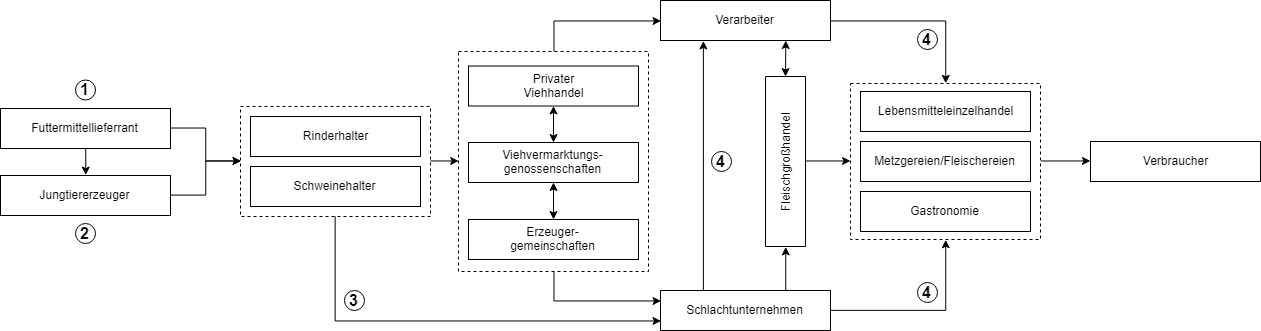
\includegraphics[width=1.0\linewidth]{pictures/structure-value-chain-meat-industry-numbered}
        \caption[Struktur der Wertschöpfungskette der Fleischwirtschaft]{Struktur der Wertschöpfungskette der Fleischwirtschaft nach \citet{Petersen2010, Voss2010, Beck2008}}
        \label{fig:structure-value-chain-meat-industry-numbered}
    \end{figure}
\end{landscape}

\noindent
Der Warenstrom beginnt mit (1) der Futtermittellieferung an die Jungtiererzeuger und Viehhalter. Jeder Betrieb wird dabei über die \ac{iln} global eindeutig identifiziert. (2) Nach der Aufzucht der Jungtiere werden diese durch Transportunternehmen zu den Viehhaltern transportiert. In den Mästbetrieben bleiben die Tiere dann bis zur Schlachtreife. (3) Im Auftrag der Schlacht- und Zerlegebetriebe werden die schlachtreifen Tiere von den Mästbetrieben angeliefert. Nach der Verarbeitung der Tiere in den Schlacht- und Zerlegebetrieben werden diese (4) an die verschiedenen Abnehmer geliefert, um letztendlich zu Produkten für den Verbraucher weiterverarbeitet zu werden. Hieraus ergibt sich, dass mindestens an den erwähnten vier Punkten der Wertschöpfungskette eine Prozessschnittstelle vom Blockchain Netzwerk bedient werden können muss.

\subsubsection{Informationswege in der Fleischindustrie}

Abbildung \ref{fig:data-stream-meat-industry} zeigt den nachfolgend beschriebenen Datenstrom zwischen den einzelnen Produktionsstufen der Fleischindustrie. \textcolor{red}{Referenz zu Anforderungen} (1) Jungtiererzeuger und Viehhalter senden jeweils eine Futtermittelbestellung an den Futtermittellieferanten. (2) Nach erfolgreicher Lieferung informiert der Futtermittellieferant den privaten Viehhandel bzw. die Viehvermarktungsgenossenschaften respektive Erzeugergemeinschaften. Die Viehhalter melden einerseits (3) die Aufnahme der Jungtiere und andererseits (4) die schlachtreife von Tieren an die Viehvermarktungsgenossenschaften zur Weitervermittlung and die Schlacht- und Zerlegebetriebe. (5) Bei der Weitervermittlung werden die Informationen über die Tiere an Schlacht- und Zerlegebetriebe übermittelt. (6) Mit dem Lieferauftrag initiiert das Schlachtunternehmen die Bestellung und den Transport der schlachtreifen Tiere. (7) Die Viehvermarktungsgenossenschaften bestätigen den Lieferauftrag mit einer elektronischen Ankündigung der Schlachtviehlieferung. Bei der Anlieferung der Tiere gleicht das Schlachtunternehmen die tatsächliche angelieferte Anzahl mit der bestellten Menge ab und meldet die Werte an die Viehvermarktungsgenossenschaften zurück. Mit dieser Wareneingangsmeldung kann die Viehvermarktungsgenossenschaft den Bestand und die aktuellen Standorte der Tiere aktualisieren. (9) Im Schlachtunternehmen werden dann weitere Informationen zu den Stammdaten der Tiere erfasst. Dazu zählen die \ac{vvvo}-Nummern der Landwirte, eine Vergabe Partie-Nummer je Lkw und eine fortlaufende Schlachtnummer. (10)Anschließend werden die Informationen wieder an die Viehvermarktungsgenossenschaft zurück gemeldet. (11) Letztendlich bedienen die Schlacht- und Zerlegebetriebe die Bestellungen der Fleischwerke, Lebensmitteleinzelhandel, Metzgereien und die Gastronomie. (12) Hier werden dann auch die letzten Stammdaten zu den Produkten erfasst und verknüpft wie beispielsweise Artikelbezeichnung, Stückzahl, Schlachtdatum und Schlacht-Nummer. (13) Mit der Zuordnung der zuverarbeitenden Fleischerzeugnisse zum Lieferschein in einem \ac{erp}-System enden die betrachteten Informationswege in der Fleischindustrie.

\begin{figure}[H]
	\centering
	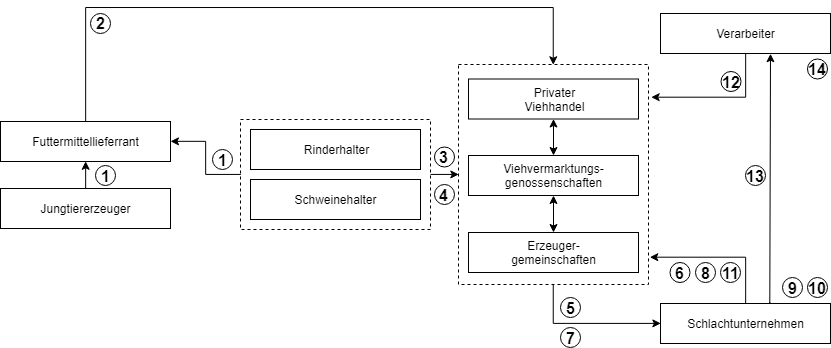
\includegraphics[width=1\linewidth]{pictures/data-stream-meat-industry-numbered}
	\caption[Datenströme innerhalb der Wertschöpfungskette]{Datenströme innerhalb der Wertschöpfungskette \textcolor{red}{QUELLE}}
	\label{fig:data-stream-meat-industry}
\end{figure}

%1 Futtermittelbestellung\\
%2 Meldung über Futtermittellieferung (DESADV optional)\\
%3 Aufnahmemeldung der Jungtiere\\
%4 Meldung schlachtreifer Schweine\\
%5 Weitervermittlung schlachtreifer Schweine an Schlachthof\\
%6 Lieferauftrag\\
%7 elektronische Ankündigung der Schlachtviehlieferung\\
%8 Wareneingangsmeldung (optional)\\
%9 Erfassung VVVO Landwirt, Vergabe Partie-Nr. je Lkw (je vom Schlachthof); Aufbringen einer fortlaufenden Schlacht-Nr. (manuell)\\
%10 Meldung Schlachtdaten\\
%11 Bestellung Schweinehälften\\
%12 u.a. Artikelbezeichnung, Stückzahl, Schlachtdatum, Schlacht-Nr., Schadenskennzeichen\\
%13 Automatische Zubuchung Schweinehälfte und Gewicht, Automatische Verknüpfung mit Lieferschein im ERP-System

\subsection{Geschäftsprozess Chargenrückverfolgung}
Die vorrangegangene Betrachtung der Waren- und Datenströme macht deutlich an welchen Schnittpunkten der Wertschöpfungskette Informationen gesammelt und zentral über die Viehvermarktungsgenossenschaften verwaltet werden. Dies ist wichtig für den Geschäftsprozess der Chargenrückverfolgung, da eine lückenlose Rückverfolgbarkeit nur dann gewährleistet ist wenn vom Erzeuger bis zum Endverbraucher alle Informationen konsistent und transparent zur Verfügung stehen. Dabei spielt es keine Rolle von welcher Seite der Wertschöpfungskette eine Rückverfolgung durchgeführt wird im Sinne des Down- und Uptracing.

Der Vergleich zwischen dem Prozess der Rückverfolgung wie er aktuell durchgeführt wird (Ist-Prozess) und wie er mit dem Einsatz eines Blockchain Systems aussehen kann (Soll-Prozess) dient dazu die funktionalen Anforderungen ableiten zu können.

\paragraph{Ist-Prozess}
Der Ist-Prozess durchläuft die Schritte von der Verbrauchermeldung bis zur Information der anderen Teilnehmer in der Wertschöpfungskette. Dabei wird anhand der Produktkennung und Verbrauchermeldung ermittelt zu welcher Produktcharge die Meldung gehört. Hierfür wird eine vielzahl an Software und Datenbeständen benötigt. Dazu zählt die Office Suite von Microsoft und ein ERP-System in Kombination mit einer Lieferantenmanagement- (SAP SRM) und Vertriebslösung (SAP CRM). Nach der Zuordnung der Verbrauchermeldung zur Produktcharge wird im Sinne des Uptracing die Charge bis zum Erzeuger zurückverfolgt, um zu prüfen in welchem Produktionsschritt das gemeldete Problem entstanden ist. Hierdurch können Maßnahmen zum Abstellen des Problem erarbeitet werden, die an alle Teilnehmer übermittelt werden. Die Chargeninformationen werden bereitsgestellt von einer zentralen Instanz, der Viehvermarktungsgenossenschaft. Dies bedeutet, liegen der Viehvermarktungsgenossenschaft lückenhafte bzw. manipulierte Datensätze vor besteht die Gefahr eine Rückverfolgung nicht vollständig durchführen zu können. Ebenfalls muss der Verbraucher der Viehvermarktungsgenossenschaft vertrauen für vollständig- und korrektheit der bereitgestellten Informationen. Nachdem alle Teilnehmer informiert sind ist der Prozess der Rückverfolgung abgeschlossen. Entsprechende folge Prozesse für einen eventuellen Rückruf von Produkten werden beim Abschluss der Rückverfolgung teils automatisch teils manuell ausgelöst.

\begin{figure}[H]
	\centering
	
\includegraphics[width=1\linewidth]{pictures/business-process-epc-diagram-bw}
	\caption[Darstellung des Geschäftsprozess Chargenrückverfolgung in eEPK Notation]{Darstellung des Geschäftsprozess Chargenrückverfolgung in eEPK Notation}
	\label{fig:business-process-epc-diagramm}
\end{figure}

\paragraph{Soll-Prozess}
Während im Ist-Prozess (Abbildung \ref{fig:target-business-process}) viele verschiedene IT-Systeme zum Einsatz kommen um alle Chargeninformationen zusammenzutragen, wird im Soll-Prozess das Blockchain Netzwerk und darauf aufsetzende dezentrale Applikationen genutzt. Betrachtet man die einzelnen Prozessschritte so ändert sich bei dem Einsatz einer Blockchain oberflächlich nichts, bei näherer Betrachtung wird dann allerdings deutlich, dass sämtliche Informationen zur Rückverfolgung der Charge vom Blockchain Netzwerk zur Verfügung gestellt werden und nicht in einzelnen Datensilos liegen wie im Ist-Prozess. So dient die Blockchain als gemeinsame Datenbasis für sämtliche Informationen die während der Produktion vom Erzeuger bis zum Lebensmitteleinzelhandel erhoben werden. Änderungen werden transparent in der Blockchain erfasst und sind durch den Konsensmechanismus vor nachträglicher Manipulation geschützt. 

\begin{figure}[H]
	\centering
	
\includegraphics[width=1\linewidth]{pictures/business-process-epc-diagram-bw}
	\caption[Darstellung des Geschäftsprozess Chargenrückverfolgung in eEPK Notation]{Darstellung des Geschäftsprozess Chargenrückverfolgung in eEPK Notation}
	\label{fig:target-business-process}
\end{figure}

\subsection{Funktionale Anforderungen}
1. Alle funktionalen Anforderungen textuell beschreiben und wo sie hergeleitet sind, immer mit Referenz auf die Tabelle in der die Übersicht aller funktionaler Anforderungen zu finden ist.

\begin{table}[H]
    \begin{tabularx}{\textwidth}{@{}lXp{2cm}@{}}
        \toprule
        ID                & Anforderung & Quelle \\
        \midrule
        \textbf{A1.1}              & Das Gesamtsystem muss fähig sein den Lebenszyklus eines Tieres vom Erzeuger bis zum Lebensmitteleinzelhandel abzubilden.                    & \textit{Wissensch. Kontext}                \\ \addlinespace
        \multicolumn{1}{r}{A1.1.1} & Das Gesamtsystem muss fähig sein Tiere anzulegen/registrieren.                     &                 \\ \addlinespace
        \multicolumn{1}{r}{A1.1.2} & Das Gesamtsystem muss fähig sein Tiere und Chargen einander zuzuordnen.                     &                 \\ \addlinespace
        \multicolumn{1}{r}{A1.1.3} & Das Gesamtsystem muss fähig sein Tiere zwischen Teilnehmern zu transferieren im Sinne eines Eigentumswechsel.                     &                 \\
        \textbf{A1.2}              & Das Gesamtsystem muss eine generische Schnittstelle zur Kommunikation mit dem Ledger anbieten.                     & \textit{Partner}                \\ \addlinespace
        \textbf{A1.3}              & Das Gesamtsystem muss fähig sein Transaktionsdaten manipulationssicher speichern zu können.                     & \textit{Partner}                \\ \addlinespace
        \textbf{A1.4}              & Das Gesamtsystem muss fähig sein den Lebenszyklus einer Charge abzubilden.                     & \textit{Partner}                \\ \addlinespace
        \multicolumn{1}{r}{A1.4.1} & Das Gesamtsystem muss fähig sein Chargen anzulegen.                     &                 \\ \addlinespace
        \multicolumn{1}{r}{A1.4.2} & Das Gesamtsystem muss fähig sein Chargen und Tiere einander zuzuordnen.                     &                 \\ \addlinespace
        \bottomrule
    \end{tabularx}
    \caption{Funktionale Anforderungen}
    \label{tab:functional-requirements}
\end{table}

\subsection{Rahmenbedingungen}
1. Alle Rahmenbedingungen textuell beschreiben und wo sie hergeleitet sind, immer mit Referenz auf die Tabelle in der die Übersicht aller Rahmenbedingungen zu finden ist.

\begin{table}[H]
    \begin{tabularx}{\textwidth}{@{}lXp{2cm}@{}}
        \toprule
        ID                & Anforderung & Quelle \\
        \midrule
        \textbf{A2.1}              & Der Prototyp muss mit der Hyperledger Fabric Blockchain Technologie konzipiert und implementiert werden.                     & \textit{Partner}                \\ \addlinespace
        \textbf{A2.2}              & Der Prototyp bildet die Teilnehmer der Wirtschöpfungskette vom Erzeuger bis zum Lebensmitteleinzelhandel ab.                     & \textit{Partner}                \\ \addlinespace
        \textbf{A2.3}              & Der Prototyp fokussiert sich bei der Transaktionsabwicklung auf die Tierart Schwein. (Verminderte Komplexität)                     & \textit{Partner}                \\ \addlinespace
        \bottomrule
    \end{tabularx}
    \caption{Funktionale Anforderungen}
    \label{tab:functional-requirements}
\end{table}

\subsection{Qualitätsanforderungen}
1. Alle Qualitätsanforderungen textuell beschreiben und wo sie hergeleitet sind, immer mit Referenz auf die Tabelle in der die Übersicht aller Qualitätsanforderungen zu finden ist.

\begin{table}[H]
    \begin{tabularx}{\textwidth}{@{}lXp{2cm}@{}}
        \toprule
        ID                & Anforderung & Quelle \\
        \midrule
        \textbf{A3.1}              & Die Architektur des Systems muss eine nachträgliche Erweiterung ermöglichen, um weitere Geschäftszweige abbilden zu können.                     & \textit{Wissensch. Kontext}                \\ \addlinespace
        \textbf{A3.2}              & Die Architektur des Systems muss mindestens eine konstante Performance bei steigender Teilnehmerzahl.                     & \textit{Partner}                \\ \addlinespace
        \textbf{A3.3}              & Das System muss auch bei Ausfall oder Komprimitierung eines oder mehrerer Teilnehmer konsistent und stabil weiter arbeiten.                    & \textit{Partner}                \\ \addlinespace
        \bottomrule
    \end{tabularx}
    \caption{Funktionale Anforderungen}
    \label{tab:functional-requirements}
\end{table}

\subsection{Systementwurf gemäß Architekturkonzept}
Unter berücksichtigung der Resultate aus Kapitel \ref{solution-concept} im Kontext des Anwendungsfalls ergibt sich die Grobarchitektur für das System wie in Abbildung \ref{fig:high-level-architecture} dargestellt.

\begin{figure}[H]
	\centering
	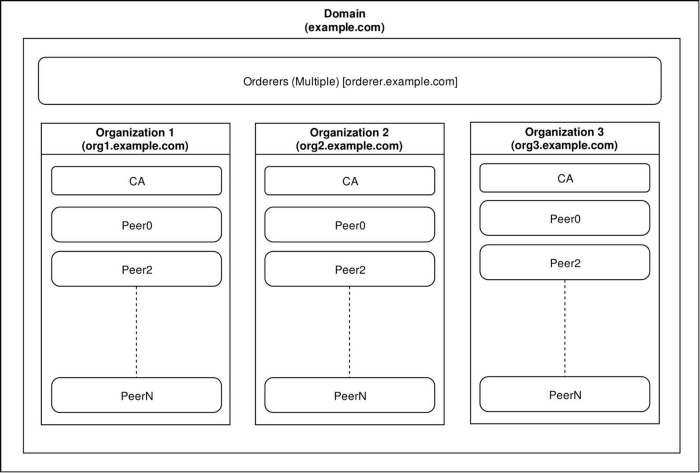
\includegraphics[width=1\linewidth]{pictures/hyperledger-fabric-architecture}
	\caption[High Level System Architecture]{High Level System Architecture}
	\label{fig:high-level-architecture}
\end{figure}

Danach besteht das Gesamtsystem aus logischer Sicht aus dem \textit{Ledger}, einer \textit{Zustandsdatenbank}, den \textit{Smart Contracts} (Chaincode), dem \textit{Konsensmechanismus}, den einzelnen \textit{Teilnehmern} und dem \textit{User Interface}. \textit{Ledger}, \textit{Zustandsdatenbank} und \textit{Smart Contracts} werden zusammen als \textit{Peer} bezeichnet. Zusätzlich gibt es noch eine Sicherheitsstrategie (\textit{CA}) zum Schutz der einzelnen Komponenten. Jeder Teilnehmer des Systems muss mindestens einen \textit{Peer} betreiben, um Transaktionen im Netzwerk erstellen und validieren zu können. Nachfolgend werden die einzelnen Komponenten beschrieben.

\subsubsection{Ledger/Konsens}
Aufbau Ledger (Chain + CouchDB)\\
Transaction Flow mit pBFT\\
1.1 Ledger\\
1.2 Channels\\
1.3 Smart Contracts\\
1.4.4 Endorsement Policies\\
1.4.5 Gossip Protocol\\
2.1 CA\\
2.2 Peers\\
2.2.1 Endorser\\
2.2.2 Anchor\\
2.2.3 General\\
2.3 Orderer\\
5 Transaction Flow\\
5.1 Endorsement\\
5.2 Ordering\\
5.3 Validation

\begin{figure}[H]
	\centering
	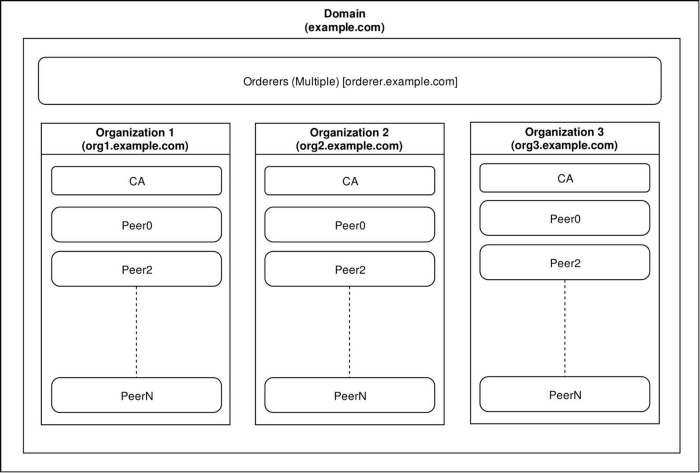
\includegraphics[width=1\linewidth]{pictures/hyperledger-fabric-architecture}
	\caption[Hyperledger Fabric Architecture]{Hyperledger Fabric Architecture (eigene Darstellung)}
	\label{fig:hyperledger-fabric-architecture}
\end{figure}

\begin{figure}[H]
	\centering
	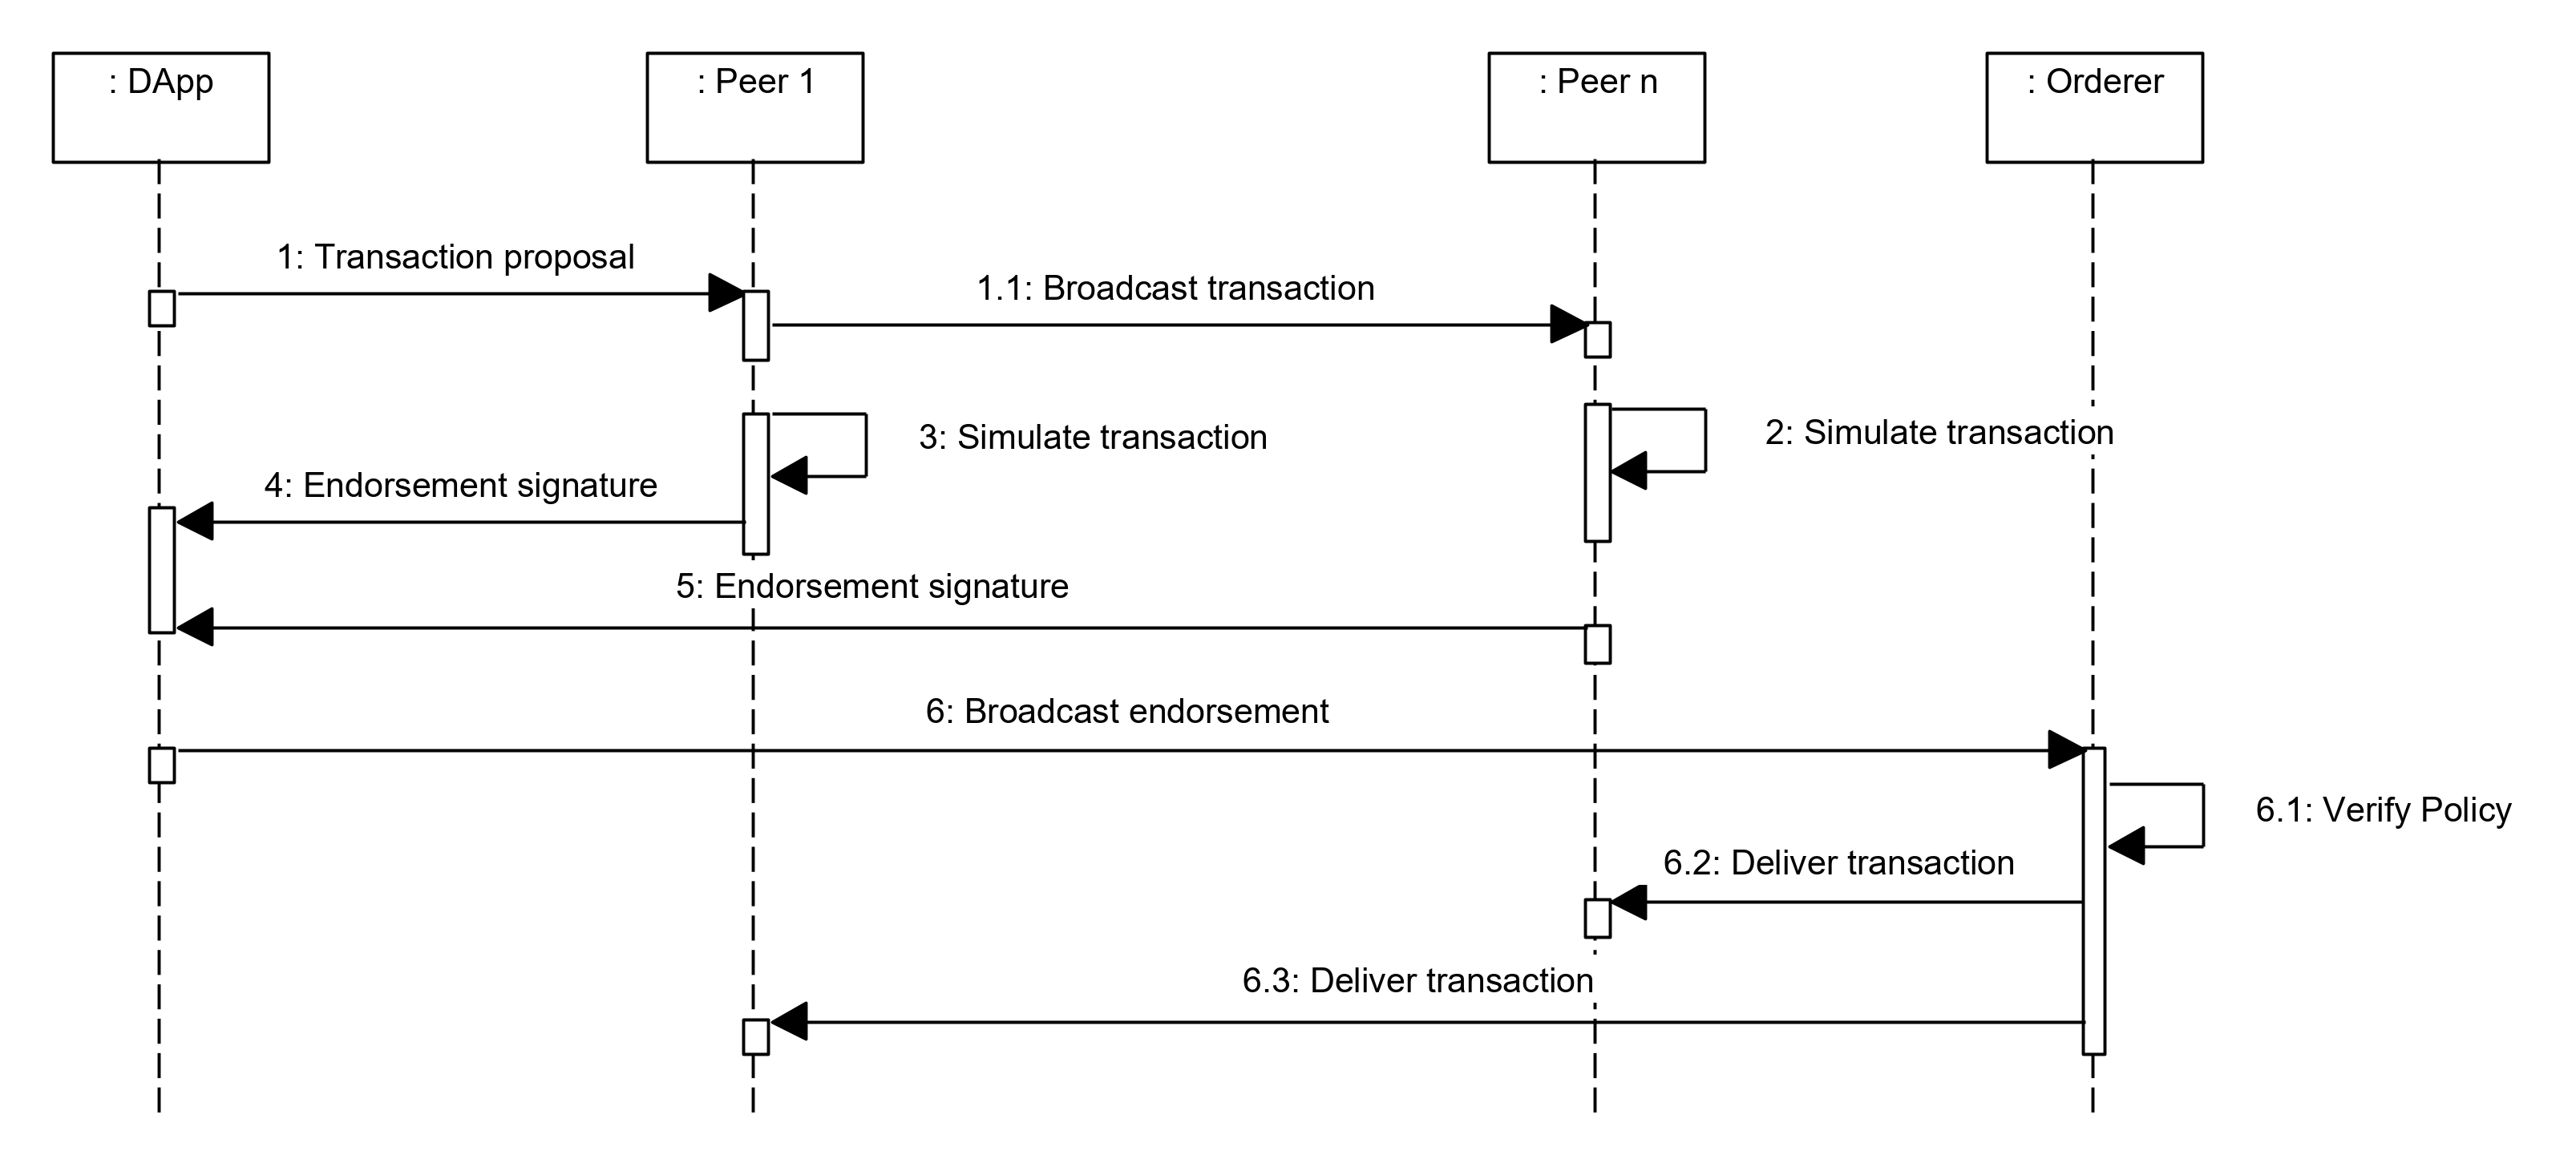
\includegraphics[width=1\linewidth]{pictures/transaction-flow}
	\caption[Transaction Flow]{Transaction Flow in Anlehnung an \citep{Choudhury2018}}
	\label{fig:transaction-flow}
\end{figure}

\subsubsection{Smart Contracts / Business Netzwerk Modell}
Klassendiagramm für Smart Contracts(Transaction Processors), Participants, Assets\\
1.4.2 Assets\\
1.4.3 Transactions\\
1.4.4 Participants

\subsubsection{Identity Management}
PKI\\
1.4.1 Organizations

\subsubsection{API (REST)}
Endpoint Beschreibung\\
3.1 REST API

\subsubsection{User Interface / \DH Apps}
Mockups

\subsubsection{Security / Permissions / Access-Control-List}
Permissions.acl Vorgaben\\
4.1 MSP

\subsection{Zusammenfassung Systementwurf}
1. Anforderungsschema wurde beschrieben\\
2. Ziele wurden erläutert\\
3. Wertschöpfungskette und Geschäftsprozesse wurden dargestellt\\
4. Rahmenbedingungen und Qualitätsanforderungen wurden beschrieben\\
5. Funktionale Anforderungen wurden festgehalten\\
6. Systementwurf wurde dokumentiert\\
7. Ausblick nächstes Kapitel auf konkrete technische Umsetzung

\newpage

\section{Technische Umsetzung} \label{sec:technical-implementation}
In diesem Kapitel wird die Umsetzung des modellierten Systementwurfs als prototypische Implementierung im Detail beschrieben. Es gibt einen Einblick in den Prozess der Konfiguration eines Blockchain Netzwerks, das mehrere Unternehmen umfasst. Dabei wird Eingangs auf die zugrunde liegende Architektur des Business Netzwerks bezug genommen. Aufbauend auf dem Fundament des Business Netzwerks werden Geschäftslogik und Berechtigungssystem erläutert.

\subsection{Business Netzwerk}
Als Basis des Blockchain Systems dient ein Hyperledger Fabric Netzwerk. Alle Dienste des Netzwerks werden in einer virtualisierten Umgebung bereitstellt. Dazu wird die Container Technologie von Docker\footnote{Docker basiert auf Linux Techniken wie \textit{Cgroups} und \textit{Namespaces}, um isolierte Umgebungen innerhalb eines Hostsystems bereitzustellen \citep{Bengel2008,Oeggl2019}.} verwendet. Zum einen bietet sich die Container Technologie zur Umsetzung eines Prototyps an, da sie sehr viel flexibler und leichtgewichtiger ist als die konventionelle Virtualisierung über Virtuelle Maschinen \citep{Ahmed2018}. Zum anderen sind die Basis Komponenten zum aufspannen eines Hyperledger Fabric Netzwerks bereits von der Linux Foundation als Container Abbild bereitgestellt, was die Realisierung des Prototypen signifikant beschleunigt. Im folgenden wird die technische Umsetzung eines Peer Knotens mittels Docker beispielhaft beschrieben. Die anderen Systemkomponenten (siehe Kapitel \ref{system-design-concept}) verhalten sich vom Aufbau her äquivalent zu einem Peer Knoten, sie sind lediglich unterschiedlich konfiguriert um verschiedene Aufgaben auszuführen. Die Netzwerke beider Unternehmen werden in diesem Fall auf der selben Maschine betrieben. In einem produktiven Umfeld würde jedes Unternehmen seine eigene Umgebung bereitstellen.

Das Prototyp Netzwerk umfasst zwei Organisationen: \textit{Org1} und \textit{Org2}. Das Unternehmen \textit{Org1} verwendet den Domänennamen \textit{org1.example.com}. Der \acf{msp} für \textit{Org1} wird als \textit{Org1MSP} bezeichnet. Das Unternehmen \textit{Org2} verwendet den Domänennamen \textit{org2.example.com}. Der \acf{msp} für \textit{Org2} heißt \textit{Org2MSP}.

\paragraph{Netzwerk Komponenten}$~~$\\
Das Hyperledger Fabric Netzwerk besteht insgesamt aus den folgenden Komponenten und Schnittstellen:

\begin{itemize}
    \item Zwei Peer Knoten für \textit{Org1}
    \begin{itemize}
        \item \textit{peer0.org1.example.com}
        \item \textit{peer1.org1.example.com}
    \end{itemize}
    \item Eine \ac{ca} für \textit{Org1} (\textit{ca.org1.example.com})
    \item Zwei Peer Knoten für \textit{Org2}
    \begin{itemize}
        \item \textit{peer0.org2.example.com}
        \item \textit{peer1.org2.example.com}
    \end{itemize}
    \item Eine \ac{ca} für \textit{Org2} (\textit{ca.org2.example.com})
    \item Ein einzelner Orderer Peer (\textit{orderer.example.com})
\end{itemize}

\noindent
Jede dieser Komponenten stellt einen Docker Container dar und ist auf Netzwerkebene über seinen Hostnamen ansprechbar. Die gesamte Netzwerkkommunikation ist über das \ac{tls}-Protokoll\footnote{\ac{tls} ist ein hybrides Verschlüsselungsprotokoll, um Datenübertragungen vor Angriffen zu schützen \citep{RFC5246}.} abgesichert. Aus diesem Grund müssen alle Zertifikate der \ac{ca} auf dem Hostsystem zur Verfügung stehen, damit eine Kommunikation mit dem Netzwerk stattfinden kann. Für Organisation \textit{Org1} ist ein Administrator User angelegt mit Namen \textit{Admin@org1.example.com}. Ebenfalls ist für Organisation \textit{Org2} ein Administrator User angelegt der \textit{Admin@org2.example.com} heißt. Zusätzlich zu den Administrator Usern der Organisationen ist die \ac{ca} mit einem Standard User konfiguriert. Der \ac{ca} User besitzt im gegensatz zu den Administrator Usern keine Berechtigungen, um Smart Contracts (Chaincode) auf Peers des Netzwerk zu installieren. Damit die Peer Administatoren sich mit dem Netzwerk verbinden können wird ein Verbindungsprofil benötigt. In diesem Verbindungsprofil werden alle Komponenten des Netzwerks definiert und die zugehörigen \ac{tls} Zertifikate hinterlegt (siehe Anhang \ref{lst:connection-profile}). Verbindungsprofil und die digitale Identität des Administrator Users, bestehend aus Zertifikat und privatem Schlüssel, bilden zusammen die sogenannte \textit{Business Network Card}. Hiermit kann sich der Administrator User über eine Hyperledger Fabric \ac{cli} mit dem Netzwerk verbinden und Befehle absetzen.

\begin{figure}[H]
	\centering
	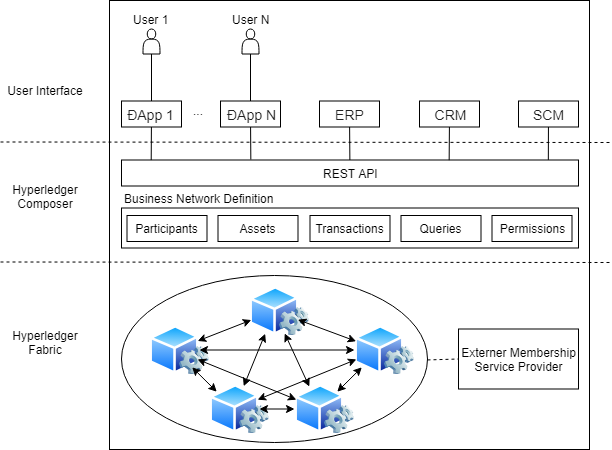
\includegraphics[width=1\linewidth]{pictures/poc-food-chain-traceability}
	\caption[Gesamtsystem Prototyp]{Gesamtsystem Prototyp}
	\label{fig:poc-food-chain-traceability}
\end{figure}

Nachdem starten der Docker Container lässt sich ein einfacher Smoke Test\footnote{Mit einem Smoke Test sollen grundlegende Probleme bei einer Software oder einem System offengelegt werden, bevor die Entwicklung von folge Komponenten begonnen wird \citep{Everett2007}.} durchführen, um sicherzustellen das das Netzwerk ordnungsgemäß hochgefahren wurde und alle Knoten arbeiten. Docker bietet zum Mangement der Container ein \ac{cli} an. Hiermit lässt sich der Smoke Test mit einem Einzeiler auf dem Terminal ausführen. Damit ist die Basiskonfiguration des Systems abgeschlossen und das Peer Netzwerk ist aufgespannt (siehe Abbildung \ref{fig:poc-food-chain-traceability} Abschnitt \textit{Hyperledger Fabric}). Im aktuellen Zustand kann das Netzwerk noch keine Transaktionen erzeugen oder verarbeiten. Dazu muss erst noch die im nächsten Kapitel beschriebene Geschäftslogik durch einen Administrator User auf einem Peer Knoten des Unternehmens installiert und instantiiert werden.

\subsection{Smart Contracts}
Smart Contracts heißen im Hyperledger Model \textit{Chaincode}. Sie setzen sich aus vier Elementen zusammen. Model, Logik, Zugriffskontrolle und Abfragedefinition bilden das sog. \acf{bna}. Das \ac{bna} lässt sich in jedes mit Hyperledger Fabric aufgespannte Blockchain Netzwerk deployen. Die Funktionsweise eines Smart Contracts soll hier am Beispiel des Eigentumswechsels eines Materials näher erläutert werden. Dazu wird auf jedes der vier Elemente eines \ac{bna} eingegangen, um den strukturellen Aufbau zu zeigen. Im Sinne des Models werden ein \textit{Participant}, ein \textit{Asset} und eine \textit{Transaction} mit einem \textit{Event} definiert wie in Listing \ref{lst:example-model-definition}. Die eigentliche Verarbeitungslogik wird gesondert von der Datenstruktur definiert (Listing \ref{lst:transaction-logic-change-ownership}). In diesem Fall wurde die Logik in der Programmiersprache JavaScript implementiert.

\begin{lstlisting}[caption={Model Example Definition},label=lst:example-model-definition]
namespace io.dev.foodchain

abstract participant Company identified by gln {
    o String gln
    o String name
}

participant Farmer extends Company {}

asset Material identified by materialId {
    o String materialId
    --> Company owner optional
}

transaction changeMaterialOwnership {
    --> Material material
    --> Company newOwner
}

event notification {
    --> Material changedMaterial
}
\end{lstlisting}

Zeile 1 in Listing \ref{lst:example-model-definition} definiert einen Namensraum für das gesamte Model. In einem produktiven Scenario würde ein Model erheblich größer sein, als das im Prototyp verwendete vereinfachte Model. Damit bei steigender Komplexität des abzubildenden Models Überblick und Wartbarkeit erhalten bleiben lässt sich das Model über mehrere Dateien abbilden und über den Namensraum auf logischer Ebene miteinander verknüpfen. Zeile 3 bis einschließlich Zeile 6 zeigt die Definition der abstrakten Klasse \textit{Company} vom Typ \textit{Participant}. Diese Definition wird in Zeile 10 konkret ausgeprägt durch die Klasse \textit{Farmer}. Äquivalent dazu werden auch alle anderen Teilnehmer der Wertschöpfungskette implementiert. Zeile 10 bis Zeile 14 zeigt die Implementierung des Assets \textit{Material}. Über die Eigenschaft \textit{owner} (Zeile 12) wird ein \textit{Material} später immer einem eindeutigen Besitzer zugeordnet. Die Eigenschaft \textit{owner} wurde dabei als direkte Ressourcenverknüpfung implementiert. Eine Ressourcenverknüpfung im Hyperledger Model lässt sich mit einer Fremdschlüsselbeziehung in einem relationalen Datenbankschema vergleichen. Die Eigenschaft kann in diesem Fall nur Werte annehmen, die eine gültige Ausprägung der abstrakten Klasse \textit{Company} darstellen und damit auch allen konkreten Ausprägungen dieser Klasse.

Um das Beispiel einfach und verständlich zu halten wurden die Definitionen der \textit{Participants} und \textit{Assets} in verkürzter Form abgebildet. Das vollständige Prototypen Model befindet sich im Anhang \ref{lst:hlc-model-definition}. Eine \textit{Transaction} mit zugehörigem \textit{Event} ist in Zeile 15 bis 22 dargestellt. Die \textit{Transaction} definiert dabei zwei Parameter als Ressourcenverknüpfung. Es werden das Asset \textit{material} sowie der neue Eigentümer \textit{newOwner} benötigt. Das \textit{Event} definiert nur einen Parameter und zwar eine Ressourcenverknüpfung zum angepassten Asset \textit{changedMaterial}. Wird das Event emittiert kann der Empfänger über die Ressource alle Informationen des Vorgangs nachvollziehen. In angebundenen \ac{ui} Applikationen kann dann auf das Event entsprechend reagiert werden bzw. können Drittsysteme beispielsweise Workflowprozesse auslösen.

\begin{lstlisting}[caption={Transaction Processor Function \textit{changeMaterialOwnership(tx)}},language=ES6,label=lst:transaction-logic-change-ownership]
/**
* Change material ownership transaction
* @param {io.dev.foodchain.changeMaterialOwnership} tx
* @transaction
*/
async function changeMaterialOwnership(tx) {
    const oMaterial = tx.material;
    const oNewOwner = tx.newOwner;
    const oActualOwner = tx.material.owner;

    const oMaterialRegistry = await getAssetRegistry(NS + '.Material');
    const bMaterialExists = await oMaterialRegistry.exists(oMaterial.getIdentifier());
    if(!bMaterialExists) {
        throw new Error('Input material does not exist.');
    }
    if (oMaterial.owner !== getCurrentParticipant()) {
        throw new Error('You are not allowed to change asset.');
    }
    const oParticipantRegistry = await getParticipantRegistry(oNewOwner.getNamespace());
    const bNewOwnerExists = await oParticipantRegistry.exists(oNewOwner.getIdentifier());
    if(!bNewOwnerExists) {
        throw new Error('New owner does not exist.');
    }

    oMaterial.ownerHistory.push(oActualOwner);
    oMaterial.owner = oNewOwner;
    await oMaterialRegistry.update(oMaterial);

    const oNotification = getFactory().newEvent('io.dev.foodchain', 'notification');
    oNotification.changedMaterial = oMaterial.getIdentifier();
    emit(oNotification);
}
\end{lstlisting}

Damit ein \textit{Participant} Funktionen auf einem \textit{Asset} ausführen kann wurden im vorherigen Abschnitt \textit{Transactions} modelliert. Zu jeder \textit{Transaction} Definition im Modell gehört eine Logikimplementierung. Verknüpft wird die Modelldefinition mit der Implementierung über die Annotation \textit{@transaction}. Eine \textit{Transaction} Funktion hat als einzigen Parameter das \textit{Transaction} Objekt. Über dieses Objekt kann innerhalb der Funktion auf alle Werte der Transaktion zurückgegriffen werden. Für das Beispiel des Eigentumswechsel wurde eine Transaktion definiert, die zum einen das \textit{Material} beinhaltet und zum anderen eine Referenz auf den neuen Eigentümer (siehe Listing \ref{lst:example-model-definition} Zeile 16 f.). Der Aufbau einer \textit{Transaction} Funktion folgt stets dem Muster - Initialiseren der Eingabeparameter, Plausibilitätsprüfungen, Geschäftslogik und abschließend die optionale Event Emittierung. Das Initialisieren der Eingabewerte wurde von Zeile 8 bis Zeile 10 implementiert. Es werden alle benötigten Werte der Transaktion zu lokalen Variablen zugewiesen. Zeile 14 bis Zeile 28 deckt die Plausibilitätsprüfung ab, hier wird geprüft ob im Falle des Eigentumswechsels

\begin{itemize}
    \item das \textit{Material} im Netzwerk vorhanden ist,
    \item der Transaktionsemittent auch Besitzer des \textit{Materials} ist und
    \item ob der neue Eigentümer als \textit{Participant} im Netzwerk vorliegt.
\end{itemize}

Die eigentliche Geschäftslogik ist relativ simpel und von Zeile 31 bis 33 implementiert. Für eine spätere Rückverfolgung der Eigentumsverhältnisse wird der aktuelle Eigentümer zur Eigentümerhistorie (Eigenschaft \textit{ownerHistory}) hinzugefügt und der neue Eigentümer wird gesetzt. Danach müssen die Assetänderungen noch an das Systemregister übermittelt werden. Das Schlüsselwort \textit{await} wird verwendet, da es sich hier um einen asynchronen Aufruf handelt und in der Logik so eine Haltemarke gesetzt wird sodass auf das Ergebnis des Aufrufs gewartet wird bevor mit der weiteren Verarbeitung der Funktion fortgefahren wird. Sollten bis zu diesem Zeitpunkt keine Fehler in der Verarbeitung aufgetreten sein, wird ein \textit{Event} erzeugt, mit Daten gefüllt und emittiert.

Einfache Berechtigungsprüfungen wie in der Transaktionslogik lassen sich auch über die Zugriffskontrolle regeln. Hyperledger unterscheidet zwischen der Zugriffskontrolle für Ressourcen innerhalb des Netzwerks und der Zugriffskontrolle für Änderungen seitens der Netzwerkadministration. Um den Zugriff auf eine Ressource zu steuern wird eine Regel definiert wie in Listing \ref{lst:model-permissions}. Diese Regel sagt aus, dass sie für jeden \textit{Participant} und bei jeder Operation (Lesen, Anlegen, Ändern, Löschen) angewandt wird (Zeile 3/4). Sie gilt für alle Ressourcen aus dem Namensraum \textit{io.dev.foodchain.*} und als Bedingung wurde definiert, dass der Besitzer \textit{r.owner.getIdentifier()} der Ressource gleich dem aktuellen \textit{Participant} ist (Zeile 5/6). Ist diese Regel erfüllt wird die Operation erlaubt bzw. bei nicht erfüllen der Zugriff auf die Ressource verweigert. Es ist anzumerken, dass die Regeln in der Reihenfolge ausgewertet werden in der sie definiert sind und die erste Regel deren Bedingung erfüllt ist, bestimmt ob der Zugang gewährt oder verweigert wird. Sofern keine Regel angewandt werden kann wird der Zugriff standardmäßig verweigert.

\begin{lstlisting}[caption={Berechtigungsdefinition},label=lst:model-permissions]
rule OwnerHasFullAccessToTheirAssets {
    description: "Allow all participants full access to their assets"
    participant(p): "io.dev.foodchain.*"
    operation: ALL
    resource(r): "io.dev.foodchain.*"
    condition: (r.owner.getIdentifier() === p.getIdentifier())
    action: ALLOW
}
\end{lstlisting}

\noindent
Das letzte Element des \acf{bna} ist die Abfragedefinition. Hier können für die Verwendung innerhalb der Transaktionslogik oder direkter Anfragen über externe Anwendungen \acs{sql}-ähnliche Abfragen formuliert werden. Listing \ref{lst:model-example-query} zeigt eine einfache Abfrage, um alle Assets vom Typ \textit{Material} zu selektieren für die gilt, das die boolesche Eigenschaft \textit{bonus} den Wert \textit{wahr} hat und das die Eigenschaft \textit{type} gleich dem Parameter \textit{\_\$type} ist. Parameter die innerhalb einer Anfrage definiert werden über den Präfix \textit{\_\$} müssen beim Aufruf der Abfrage mit übergeben werden. Über den eindeutigen Namen \textit{selectBonusMaterials} lässt sich diese Abfrage direkt in der Transaktionslogik ausführen.

\begin{lstlisting}[caption={Abfragedefinition},label=lst:model-example-query]
    query selectBonusMaterials {
      description: "Select materials based on bonus condition"
      statement:
          SELECT io.dev.foodchain.Material
              WHERE (bonus == true)
              AND (type == _$type)
              ORDER BY [status ASC]
    }
\end{lstlisting}

\noindent
In der \textit{statement} Eigenschaft einer \textit{Query} können jeweils folgende Operatoren verwendet werden:

\begin{itemize}
    \item \textit{SELECT} ist ein obligatorischer Operator und definiert standardmäßig das Register und den Asset- oder Teilnehmertyp, der zurückgegeben werden soll.
    \item \textit{FROM} ist ein optionaler Operator, der ein anderes Register für die Abfrage festlegt.
    \item \textit{WHERE} ist ein optionaler Operator, der die Bedingung definiert, die auf die selektierten anzuwenden sind.
    \item \textit{AND} ist ein optionaler Operator, der zusätzliche Bedingungen definiert.
    \item \textit{OR} ist ein optionaler Operator, der alternative Bedingungen definiert.
    \item \textit{CONTAINS} ist ein optionaler Operator, der Bedingungen für Array-Werte definiert.
    \item \textit{ORDER BY} ist ein optionaler Operator, der die Sortierung der Ergebnisse definiert.
\end{itemize}

\noindent
Damit ist das \acf{bna} vollständig und kann in einem Hyperledger Fabric Netzwerk installiert und instantiiert werden. Ein Netzwerkadministrator kann anschließend \textit{Participants} erzeugen und mit der digitalen Identität verknüpfen. Der Netzwerkteilnehmer ist daraufhin in der Lage Transaktionen im Netzwerk abzusetzen, um mit dem Smart Contract zu interagieren und Geschäftsvorgänge entsprechend abzubilden.

\subsection{Schnittstelle}
Damit die Funktionalität des Blockchain Netzwerks in bestehende IT Landschaften integriert werden kann bietet Hyperledger die Möglichkeit einen Smart Contract in Form einer \acs{rest}\footnote{\acf{rest} steht für ein Programmierparadigma für verteilte Systeme. Dabei wird der Zustand einer Ressource nicht gesondert gespeichert (Session) sondern über den \ac{uri} codiert.} \acs{api} für externe Anwendungen freizugeben.

Mit dem Ansatz einer \ac{rest} \ac{api} wird die Idee einer programmiersprachen unabhängigen Schnittstelle realisiert. Nahezu jede moderne Programmiersprache ist in der Lage simple \ac{http} Anfragen zu formulieren, über das Internet abzusetzen und das Resultat auszuwerten. Dadurch kann eine breite Masse an \ac{ui} Technologien und Frameworks verwendet werden, um für den Endanwender entsprechende Applikationen zur Nutzung der Smart Contract Funktionalität zu implementieren. Ebenfalls sind externe Systeme wie beispielsweise \ac{erp}-Systeme über die \ac{rest} \ac{api} in der Lage mit dem Blockchain Netzwerk zu kommunizieren und Asset Operationen auszuführen.

Die \ac{rest} Schnittstelle wird dabei nach der \textit{OpenAPI}\footnote{OpenAPI (ursprünglich Swagger) bietet eine Spezifikation und ein Framework zum Beschreiben, Erzeugen, Konsumieren und Visualisieren von \ac{rest} Schnittstellen \citep{OAI2018, Purushothaman2015}.} Spezifikation generiert und zur Verfügung gestellt. Bei der Generierung wird aus den Modelldefinitionen und der Transaktionslogik die Klassen- und Funktionsdokumentation extrahiert und in der Schnittstellendokumention dargestellt.

Wird die \ac{rest} Schnittstellen über den Hyperledger Composer REST Server ausgeliefert erhält man eine Übersicht aller \textit{Assets, Participants, Transactions \& Queries} die über den Smart Contract abgebildet worden sind. Abbildung \ref{fig:rest-api-explorer} zeigt einen Ausschnitt der Oberfläche. Darauf sind drei \ac{api} Endpunkte abgebildet namentlich \textit{generateMockTransactionData}, \textit{Manufacturer} und \textit{Material}. Die ersten beiden Endpunkte bilden eine \textit{Transaction} und einen \textit{Participant} aus dem Smart Contract ab. Der dritte Endpunkt zeigt die Dokumentation einer \ac{http} \textit{GET} Operation für ein \textit{Material} mit Beispielwerten eines Resultats. Darunter sind alle weiteren möglichen \ac{http} Operationen inklusive des codierten \ac{uri}.

\begin{figure}[H]
	\centering
	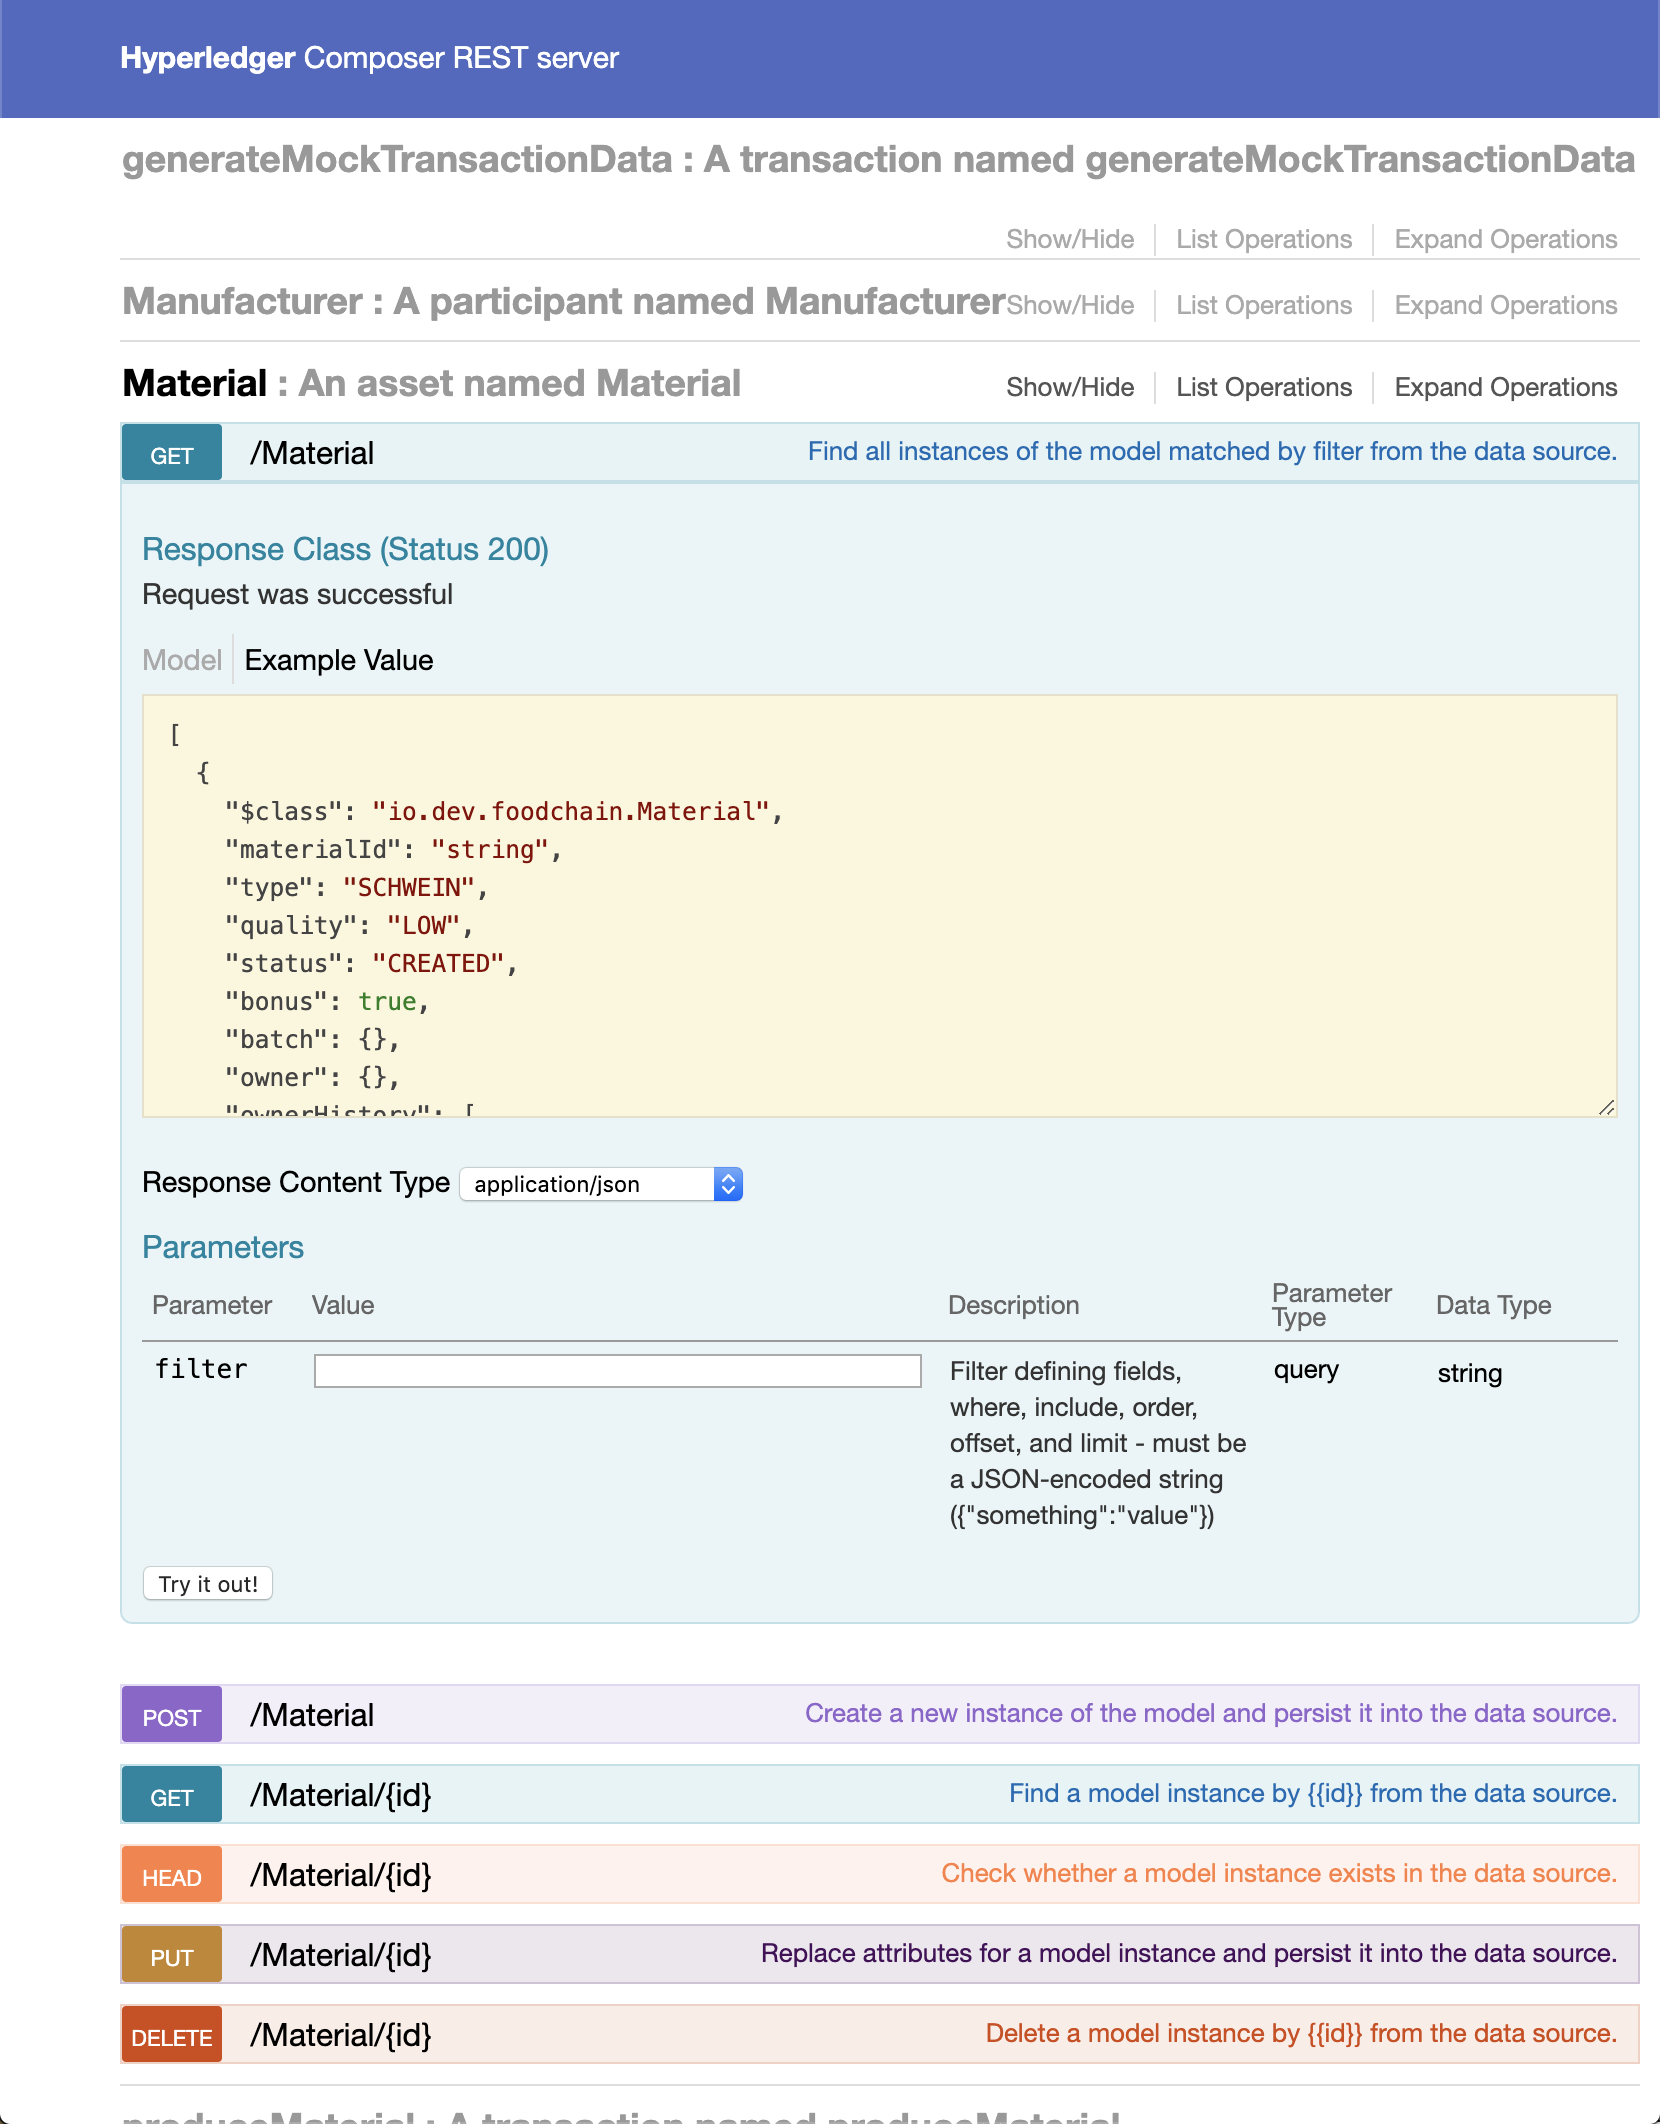
\includegraphics[width=1\linewidth]{pictures/rest-api-explorer}
	\caption[Weboberfläche der \ac{rest} \ac{api}]{Weboberfläche der \ac{rest} \ac{api}}
	\label{fig:rest-api-explorer}
\end{figure}

%3 Authentication via OAuth 2.0

\subsection{Zusammenfassung technische Umsetzung}
In diesem Kapitel wurde gezeigt wie die Basis einer Blockchain Lösung mit Hyperledger Fabric und Composer realisiert wird. Dazu wurde, wie zuvor im Systementwurf konzeptioniert, ein Peer Netzwerk aufgespannt. Darauf aufbauend ist die Geschäftslogik mit Hyperledger Composer implementiert worde. Eine Kapselung des Smart Contracts in eine \ac{rest} Schnittstelle dient dazu auch externen Anwendungen die Funktionalität des Smart Contracts bereitzustellen. Dabei wurde die \ac{rest} \ac{api} nach der \textit{OpenAPI} Spezifikation modelliert.

%Fundament mit HL Fabric gebaut, Logikschicht über HL Composer realisiert und Zugriff über standartisierte REST Schnittstelle ermöglicht.

\newpage

\section{Evaluation}
\textcolor{red}{Lorem ipsum dolor sit amet, consetetur sadipscing elitr, sed diam nonumy eirmod tempor invidunt ut labore et dolore magna aliquyam erat, sed diam voluptua. Lorem ipsum dolor sit amet, consetetur sadipscing elitr, sed diam nonumy eirmod tempor invidunt ut labore et dolore magna aliquyam erat, sed diam voluptua.}

\subsection{Experimenteller Aufbau}

\subsection{Resultate}

\subsubsection{Transaktionskosten}

\subsubsection{Transaktionsgeschwindigkeit}

\subsubsection{Datenverfügbarkeit}

\subsubsection{Innovationskraft}


\newpage


% Insert conclusion
\section{Abschlussbetrachtung} \label{sec:concluding-review}

\subsection{Zusammenfassung}

In dieser Masterarbeit wurde analysiert, wie sich eine Chargenrückverfolgung mittels der \textit{Blockchain-Technologie} realisieren lässt. Dazu wurden die in Abschnitt \ref{Problemstellung} gestellten Forschungsfragen anhand der \textit{Design Science Methode} nach \citet{Hevner2007} bearbeitet. Die einzelnen Teilfragen wurden in den Kapiteln \ref{sec:solution-concept} und \ref{sec:system-design} mit einer der Fragestellung passenden Methodik näher betrachtet. Die Forschungsfrage \textit{FF1.1} sowie \textit{FF1.2} sind über die Grundlagenkapitel abgedeckt worden. In diesen Kapiteln wurde detailliert beschrieben, welche Anforderungen und Daten zur Realisierung einer Chargenrückverfolgung in der Fleischwarenindustrie von nöten sind. Neben einer ausführlichen Beschreibung der Wertschöpfungskette im fleischverarbeitenden Gewerbe wurde die \textit{Blockchain-Technologie} und ihre Ausprägungen behandelt. Forschungsfrage \textit{FF1.3} wurde mittels einer SWOT-Analyse mit anschließender Nutzwertanalyse entgegen getreten. Aus den Ergebnissen der Analyse wurde dann im Kapitel \ref{sec:system-design} ein entsprechendes System Design abgeleitet, welches für den Anwendungsfall passend ist und die in \textit{FF1.1} ermittelten Anforderungen erfüllt. Nach dem Systementwurf folgte die prototypische Implementierung des zuvor modellierten Systems auf Basis der \textit{Hyperledger Fabric Blockchain} in Kombination mit dem \textit{Hyperledger Composer} Framework zur \textit{Smart Contract} generierung. Evaluiert wurde der Prototyp anhand eines Experteninterviews. Die Befragung einer Person mit direktem Bezug zu den behandelten Geschäftsprozessen sowie der nötigen Kompetenz bezüglich neuartiger Technologien wie \textit{Blockchain} und \ac{iot} stellt eine für diese Arbeit ausreichend gesicherte Evaluation der Ergebnisse aus Systementwurf und dem resultierenden Prototyp dar.

\subsection{Reflexion}

Während der Anforderungsanalyse hat sich gezeigt, das die \textit{Blockchain-Technologie} in den Fachabteilungen des Praxispartners zwar bekannt war, ihre möglichen Einsatzwecke jedoch noch vollkommen unklar sind. \textit{Blockchain} wurde stets mit der Kryptowährung Bitcoin assoziiert. So war es schwierig die Anforderung entsprechend spezifisch und nicht zu allgemein zu erheben ohne das wichtige Aspekte des zu modellierenden System außer acht gelassen werden. Auf Grund der Komplexität im realen Umfeld der Chargenrückverfolgung wurde der aufgenommen Prozess sowie das zu Grunde liegende Datenmodell soweit vereinfacht, das die Funktionalität der Chargenrückverfolgung weiterhin auf die Realität im Unternehmen abgestimmt war. Allerdings konnten eine Vielzahl an Sonderfällen, die grade bei der Verarbeitung von Schweinen auftreten, nicht beachtet werden. Die Vertragssituation zwischen Landwirten und den verarbeitenden Betrieben basiert oft auf mündlichen Absprachen bzw. sind hierfür großzügige Toleranzen in den Verträgen erfasst um nachträgliche Anpassungen beispielsweise bei den Preisen für bestimmte Tiere möglich zu machen. Da der Fokus dieser Arbeit auf der generellen Machbarkeit einer Chargenrückverfolgung mittels der \textit{Blockchain-Technologie} lag, wurden diese Freiheitsgrade nicht weiter betrachtet bzw. in der prototypischen Implementierung beachtet. Solch eine komplexe Wertschöpfungskette wie sie in der Fleischwarenindustrie vorliegt könnte nur schwer die im wissenschaftlichen Kontext dieser Arbeit intendierte notwendige Übertragbarkeit und Reproduzierbarkeit gewährleisten.

\subsection{Ausblick}

Aus wissenschaftlicher Perspektive bietet sich die naheliegendste Fortsetzung dieser Arbeit sicherlich in der Implementierung des vorgestellten Systementwurfs in einem konkreten betrieblichen Umfeld an. Der in dieser Arbeit entwickelte Prototyp kann hierbei als Grundlage zur Erforschung weiterer Prozesse die über eine \textit{Blockchain} abgebildet werden herangezogen werden. Dabei könnte der gezeigte Systementwurf mit entsprechendem Aufwand für weitere Tierarten, Veterinärinformationen oder Futtermitteldaten erweitert werden. Ebenfalls wäre es denkbar eine vorhandene \textit{\acf{iot}} Lösung zu integrieren, um Sensordaten aus den Betriebsstätten bzw. während des Transports direkt in die \textit{Blockchain} einfließen zu lassen. Hierdurch könnte der Informationsgehalt für Aussagen zu einer \textit{Charge} oder dem gesamten Lebenszyklus eines einzelnen Tieres vom Landwirt bis zum Endkunden noch einmal deutlich erhöht werden. Außerdem bietet sich eine Integration der Blockchaindatenbasis mit vorhandenen \ac{erp}-Systemen an. \ac{erp}-Systeme halten eine große Menge an Stamm- und Bewegungsdaten aus dem betrieblichen Kontext vor. Lassen sich diese Daten mit den Transaktionsdaten des \textit{Blockchain} Netzwerks verknüpfen eröffnen sich weitere Anwendungsgebiete beispielsweise im Bereich von Business Intelligence.

\newpage


\pagenumbering{Roman}
\setcounter{page}{7}

% Insert appendix
\appendix
%\begin{appendix}

%\addcontentsline{toc}{section}{Anhang}
%\section*{Anhang}
\section{Anhang}
\subsection*{Funktionale Anforderungen}
%\subsection*{Funktionale Anforderungen}
\begin{table}[H]
    \begin{tabularx}{\textwidth}{@{}lXp{2cm}@{}}
        \toprule
        ID                & Anforderung & Quelle \\
        \midrule
        \textbf{A1.1}              & Das Gesamtsystem muss fähig sein den Lebenszyklus eines Tieres vom Erzeuger bis zum Lebensmitteleinzelhandel abzubilden.                    & \textit{Wissensch. Kontext}                \\ \addlinespace
        \multicolumn{1}{r}{A1.1.1} & Das Gesamtsystem muss fähig sein Tiere anzulegen/registrieren.                     &                 \\ \addlinespace
        \multicolumn{1}{r}{A1.1.2} & Das Gesamtsystem muss fähig sein Tiere und Chargen einander zuzuordnen.                     &                 \\ \addlinespace
        \multicolumn{1}{r}{A1.1.3} & Das Gesamtsystem muss fähig sein Tiere zwischen Teilnehmern zu transferieren im Sinne eines Eigentumswechsel.                     &                 \\
        \textbf{A1.2}              & Das Gesamtsystem muss eine generische Schnittstelle zur Kommunikation mit dem Ledger anbieten.                     & \textit{Partner}                \\ \addlinespace
        \textbf{A1.3}              & Das Gesamtsystem muss fähig sein Transaktionsdaten manipulationssicher speichern zu können.                     & \textit{Partner}                \\ \addlinespace
        \textbf{A1.4}              & Das Gesamtsystem muss fähig sein den Lebenszyklus einer Charge abzubilden.                     & \textit{Partner}                \\ \addlinespace
        \multicolumn{1}{r}{A1.4.1} & Das Gesamtsystem muss fähig sein Chargen anzulegen.                     &                 \\ \addlinespace
        \multicolumn{1}{r}{A1.4.2} & Das Gesamtsystem muss fähig sein Chargen und Tiere einander zuzuordnen.                     &                 \\ \addlinespace
        \bottomrule
    \end{tabularx}
    \caption{Funktionale Anforderungen}
    \label{tab:functional-requirements}
\end{table}

\subsection{Rahmenbedingungen}
\begin{table}[H]
    \begin{tabularx}{\textwidth}{@{}lXp{2cm}@{}}
        \toprule
        ID                & Anforderung & Quelle \\
        \midrule
        \textbf{A2.1}              & Der Prototyp muss mit der Hyperledger Fabric Blockchain Technologie konzipiert und implementiert werden.                     & \textit{Partner}                \\ \addlinespace
        \textbf{A2.2}              & Der Prototyp bildet die Teilnehmer der Wirtschöpfungskette vom Erzeuger bis zum Lebensmitteleinzelhandel ab.                     & \textit{Partner}                \\ \addlinespace
        \textbf{A2.3}              & Der Prototyp fokussiert sich bei der Transaktionsabwicklung auf die Tierart Schwein. (Verminderte Komplexität)                     & \textit{Partner}                \\ \addlinespace
        \textbf{A2.4}\phantomsection\label{req:A2.4}              & Das Gesamtsystem muss in einer abgeschlossenen Umgebung gehosted und vor pseudonymen Zugriff geschützt sein.                     & \textit{Partner}                \\ \addlinespace
        \bottomrule
    \end{tabularx}
    \caption{Funktionale Anforderungen}
    \label{tab:functional-requirements}
\end{table}

\subsection{Qualitätsanforderungen}
\begin{table}[H]
    \begin{tabularx}{\textwidth}{@{}lXp{2cm}@{}}
        \toprule
        ID                & Anforderung & Quelle \\
        \midrule
        \textbf{A3.1}              & Die Architektur des Systems muss eine nachträgliche Erweiterung ermöglichen, um weitere Geschäftszweige abbilden zu können.                     & \textit{Wissensch. Kontext}                \\ \addlinespace
        \textbf{A3.2}              & \textcolor{red}{Die Architektur des Systems muss mindestens eine konstante Performance bei steigender Teilnehmerzahl.}                     & \textit{Partner}                \\ \addlinespace
        \textbf{A3.3}              & Das System muss auch bei Ausfall oder Komprimitierung eines oder mehrerer Teilnehmer konsistent und stabil weiter arbeiten.                    & \textit{Partner}                \\ \addlinespace
        \bottomrule
    \end{tabularx}
    \caption{Funktionale Anforderungen}
    \label{tab:functional-requirements}
\end{table}

\newpage
\subsection{Listings}
\subsubsection{Listing A}
\begin{lstlisting}[caption={Hyperledger Fabric Peer \textit{Dockerfile}},captionpos=b,language=Dockerfile,label=lst:dockerfile-hl-peer]
FROM golang:1.11.5

ENV DEBIAN_FRONTEND noninteractive
ENV FABRIC_ROOT=$GOPATH/src/github.com/hyperledger/fabric
ENV CHAINTOOL_RELEASE=1.1.2

# Architecture of the node
ENV ARCH=amd64
# version for the base images (baseos, baseimage, ccenv, etc.), used in core.yaml as BaseVersion
ENV BASEIMAGE_RELEASE=0.4.14
# BASE_VERSION is required in core.yaml for the runtime fabric-baseos
ENV BASE_VERSION=1.4.0
# version for the peer/orderer binaries, the community version tracks the hash value like 1.0.0-snapshot-51b7e85
# PROJECT_VERSION is required in core.yaml to build image for cc container
ENV PROJECT_VERSION=1.4.0
# generic golang cc builder environment (core.yaml): builder: $(DOCKER_NS)/fabric-ccenv:$(ARCH)-$(PROJECT_VERSION)
ENV DOCKER_NS=hyperledger
# for golang or car's baseos for cc runtime: $(BASE_DOCKER_NS)/fabric-baseos:$(ARCH)-$(BASEIMAGE_RELEASE)
ENV BASE_DOCKER_NS=hyperledger
ENV LD_FLAGS="-X github.com/hyperledger/fabric/common/metadata.Version=${BASE_VERSION} \
    -X github.com/hyperledger/fabric/common/metadata.BaseVersion=${BASEIMAGE_RELEASE} \
    -X github.com/hyperledger/fabric/common/metadata.BaseDockerLabel=org.hyperledger.fabric \
    -X github.com/hyperledger/fabric/common/metadata.DockerNamespace=hyperledger \
    -X github.com/hyperledger/fabric/common/metadata.BaseDockerNamespace=hyperledger \
    -X github.com/hyperledger/fabric/common/metadata.Experimental=true \
    -linkmode external -extldflags '-static -lpthread'"

# Peer config path
ENV FABRIC_CFG_PATH=/etc/hyperledger/fabric
RUN mkdir -p /var/hyperledger/db \
    /var/hyperledger/production \
    $GOPATH/src/github.com/hyperledger \
    $FABRIC_CFG_PATH \
    /chaincode/input \
    /chaincode/output

# Install development dependencies
RUN apt-get update \
        && apt-get install -y apt-utils python-dev \
        && apt-get install -y libsnappy-dev zlib1g-dev libbz2-dev libyaml-dev libltdl-dev libtool \
        && apt-get install -y python-pip \
        && apt-get install -y tree jq unzip\
        && rm -rf /var/cache/apt

# install chaintool
#RUN curl -L https://github.com/hyperledger/fabric-chaintool/releases/download/v0.10.3/chaintool > /usr/local/bin/chaintool \
RUN curl -fL https://nexus.hyperledger.org/content/repositories/releases/org/hyperledger/fabric/hyperledger-fabric/chaintool-${CHAINTOOL_RELEASE}/hyperledger-fabric-chaintool-${CHAINTOOL_RELEASE}.jar > /usr/local/bin/chaintool \
    && chmod a+x /usr/local/bin/chaintool

# install gotools
RUN go get github.com/golang/protobuf/protoc-gen-go \
    && go get github.com/maxbrunsfeld/counterfeiter \
    && go get github.com/axw/gocov/... \
    && go get github.com/AlekSi/gocov-xml \
    && go get golang.org/x/tools/cmd/goimports \
    && go get golang.org/x/lint/golint \
    && go get github.com/estesp/manifest-tool \
    && go get github.com/client9/misspell/cmd/misspell \
    && go get github.com/estesp/manifest-tool \
    && go get github.com/onsi/ginkgo/ginkgo

# Clone the Hyperledger Fabric code and cp sample config files
RUN cd $GOPATH/src/github.com/hyperledger \
    && git clone --single-branch -b release-1.4 --depth 1 http://gerrit.hyperledger.org/r/fabric \
    && cp $FABRIC_ROOT/devenv/limits.conf /etc/security/limits.conf \
    && cp -r $FABRIC_ROOT/sampleconfig/* $FABRIC_CFG_PATH/ \
    && cp $FABRIC_ROOT/examples/cluster/config/configtx.yaml $FABRIC_CFG_PATH/ \
    && cp $FABRIC_ROOT/examples/cluster/config/cryptogen.yaml $FABRIC_CFG_PATH/

# install configtxgen, cryptogen and configtxlator
RUN cd $FABRIC_ROOT/ \
    && go install -tags "experimental" -ldflags "${LD_FLAGS}" github.com/hyperledger/fabric/common/tools/configtxgen \
    && go install -tags "experimental" -ldflags "${LD_FLAGS}" github.com/hyperledger/fabric/common/tools/cryptogen \
    && go install -tags "experimental" -ldflags "${LD_FLAGS}" github.com/hyperledger/fabric/common/tools/configtxlator

# Install eventsclient
RUN cd $FABRIC_ROOT/examples/events/eventsclient \
    && go install \
    && go clean

# Install discover cmd
RUN CGO_CFLAGS=" " go install -tags "experimental" -ldflags "-X github.com/hyperledger/fabric/cmd/discover/metadata.Version=${BASE_VERSION}" github.com/hyperledger/fabric/cmd/discover

# The data and config dir, can map external one with -v
VOLUME /var/hyperledger
#VOLUME /etc/hyperledger/fabric

# temporarily fix the `go list` complain problem, which is required in chaincode packaging, see core/chaincode/platforms/golang/platform.go#GetDepoymentPayload
ENV GOROOT=/usr/local/go

WORKDIR $FABRIC_ROOT

# This is only a workaround for current hard-coded problem when using as fabric-baseimage.
RUN ln -s $GOPATH /opt/gopath
LABEL org.hyperledger.fabric.version=${PROJECT_VERSION} \
    org.hyperledger.fabric.base.version=${BASEIMAGE_RELEASE}
\end{lstlisting}

\subsubsection*{Listing B}
\begin{lstlisting}[caption={Hyperledger Fabric Network \textit{Connection Profile}},captionpos=b,language=json,label=lst:connection-profile]
    {
        "name": "hlfv1",
        "x-type": "hlfv1",
        "x-commitTimeout": 300,
        "version": "1.0.0",
        "client": {
            "organization": "Org1",
            "connection": {
                "timeout": {
                    "peer": {
                        "endorser": "300",
                        "eventHub": "300",
                        "eventReg": "300"
                    },
                    "orderer": "300"
                }
            }
        },
        "channels": {
            "composerchannel": {
                "orderers": [
                    "orderer.example.com"
                ],
                "peers": {
                    "peer0.org1.example.com": {
                        "endorsingPeer": true,
                        "chaincodeQuery": true,
                        "ledgerQuery": true,
                        "eventSource": true
                    }
                }
            }
        },
        "organizations": {
            "Org1": {
                "mspid": "Org1MSP",
                "peers": [
                    "peer0.org1.example.com"
                ],
                "certificateAuthorities": [
                    "ca.org1.example.com"
                ]
            }
        },
        "orderers": {
            "orderer.example.com": {
                "url": "grpc://orderer.example.com:7050"
            }
        },
        "peers": {
            "peer0.org1.example.com": {
                "url": "grpc://peer0.org1.example.com:7051"
            }
        },
        "certificateAuthorities": {
            "ca.org1.example.com": {
                "url": "http://ca.org1.example.com:7054",
                "caName": "ca.org1.example.com"
            }
        }
    }
\end{lstlisting}

\newpage
% \addcontentsline{toc}{section}{Literaturverzeichnis}
\section{Literaturverzeichnis}
\renewcommand{\refname}{B LITERATURVERZEICHNIS}
\bibliographystyle{apalike}
%\bibliography{thesis} % Point to BibTeX literature file e.g. literatur.bib
{\def\section*#1{}\bibliography{thesis}}

% \end{appendix}
\newpage


% Insert declaration
\section*{Abschließende Erklärung}

Ich versichere hiermit, dass ich meine Masterarbeit selbständig und ohne fremde Hilfe angefertigt habe, und dass ich alle von anderen Autoren wörtlich übernommenen Stellen wie auch die sich an die Gedankengänge anderer Autoren eng anlegenden Ausführungen meiner Arbeit besonders gekennzeichnet und die Quellen zitiert habe.

\vspace*{3cm}
\noindent Oldenburg, den \today \hspace*{2cm} Nils Lutz


\end{document}
